\documentclass[9pt,english,twoside,openright]{scrbook}
\usepackage{style/header}
% PROCESSES
\newcommand{\qcd}{\ensuremath{QCD}\xspace}
\newcommand{\wjets}{\ensuremath{\textrm{W+jets}}\xspace}
\newcommand{\zjets}{\ensuremath{\textrm{$Z/\gamma^*$+jets}}\xspace}
\newcommand{\vjets}{\ensuremath{\textrm{V+jets}}\xspace}
\newcommand{\ttbar}{\ensuremath{\mathrm{t}\bar{\mathrm{t}}}\xspace}
\newcommand{\tw}{\ensuremath{\mathrm{tW}}\xspace}
\newcommand{\tch}{\ensuremath{t\mathrm{\mbox{-}channel}}\xspace}


% VARIABLES
\newcommand{\muiso}{\ensuremath{I_\mathrm{rel.}^{\mu}}\xspace}
\newcommand{\eiso}{\ensuremath{I_\mathrm{rel.}^{e}}\xspace}
\newcommand{\mtop}{\ensuremath{m_{\mu\nu \mathrm{b}}}\xspace}
\newcommand{\mw}{\ensuremath{m_{\mathrm{W}}}\xspace}
\newcommand{\met}{\ensuremath{{E\!\!\!/}_{\mathrm{T}}}\xspace}
\newcommand{\mtw}{\ensuremath{m_{\mathrm{T}}(\mathrm{W})}\xspace}
\newcommand{\pvmiss}{\ensuremath{\vec{p_\mathrm{T}}\hspace{-1.02em}/\kern 0.5em}\xspace}
\newcommand{\bdt}{\ensuremath{\mathrm{BDT}}\xspace}
\newcommand{\bdtcut}{\ensuremath{0.2}\xspace}

%UNITS
\newcommand{\keV}{\ensuremath{\mathrm{keV}}\xspace}
\newcommand{\MeV}{\ensuremath{\mathrm{MeV}}\xspace}
\newcommand{\GeV}{\ensuremath{\mathrm{GeV}}\xspace}
\newcommand{\TeV}{\ensuremath{\mathrm{TeV}}\xspace}

\newcommand{\pb}{\ensuremath{\mathrm{pb}}\xspace}
\newcommand{\fb}{\ensuremath{\mathrm{fb}}\xspace}
\newcommand{\ab}{\ensuremath{\mathrm{ab}}\xspace}

\newcommand{\pbinv}{\ensuremath{\mathrm{pb}^{-1}}\xspace}
\newcommand{\fbinv}{\ensuremath{\mathrm{fb}^{-1}}\xspace}
\newcommand{\abinv}{\ensuremath{\mathrm{ab}^{-1}}\xspace}


% FORMATTING
\newcommand{\typew}[1]{\texttt{\detokenize{#1}}}
\newcount\colveccount
\newcommand*\colvec[1]{
    \global\colveccount#1
    \begin{pmatrix}
    \colvecnext
}
\def\colvecnext#1{
    #1
    \global\advance\colveccount-1
    \ifnum\colveccount>0
        \\
        \expandafter\colvecnext
    \else
        \end{pmatrix}
    \fi
}

% OTHER
\newcommand{\invfb}{\ensuremath{\mathrm{fb}^{-1}}\xspace}
\newcommand{\invpb}{\ensuremath{\mathrm{pb}^{-1}}\xspace}
\newcommand{\jprime}{\ensuremath{j^{\prime}}\xspace}
\newcommand{\qprime}{\ensuremath{q^{\prime}}\xspace}
\newcommand{\bjtop}{\ensuremath{j_\mathrm{b,top}}\xspace}

\newcommand{\AMCATNLO}{\textsc{mg}5\_a\textsc{mc@nlo}\xspace}
\newcommand{\tunfold}{\textsc{TUnfold}\xspace}

%\def\todolist{\subsection{TODO list}}
%\newcommand{\addtodolist}[1]{\expandafter\def\expandafter\todolist\expandafter{\todolist{}\\ #1}}
%\newcommand{\todo}[1]{\textsc{\color{red}{\textbf{TODO}: #1}}\addtodolist{#1}}
%\newcommand{\todo}[1]{}

\loadglsentries{sections/acronyms}

\begin{document}
\setupTextStyle

%\renewcommand*{\arraystretch}{1.1}
%\begin{clearedpagestyle}
\parbox[c][][c]{0.2\textwidth}{

\includegraphics[height=2.cm]{figures/title/UCL.pdf}
}\parbox[c][][c]{0.799\textwidth}{\vspace{0.05cm}
\begin{flushright}
\large Universit{\'e} catholique de Louvain\\[0.25\baselineskip]
\normalsize Secteur des Sciences et Technologies\\[0.15\baselineskip] 
Institut de Recherche en Math{\'e}matique et Physique\\[0.15\baselineskip]
Center for Cosmology, Particle Physics and Phenomenology
\end{flushright}
}
\vspace{1.5cm}
\begin{center}
%{\color{gray}\rule{\textwidth}{\myrulewidth}}
\vspace{0.3cm}
\parbox{0.95\textwidth}{
\usekomafont{chapter}\selectfont\centering
\textsf{Measurements of differential single-top-quark cross sections in \textsl{t}~channel at 8~and 13~TeV with the CMS experiment}
%\textsf{Single top quarks: Differential cross sections, polarization, and charge asymmetry measurements in \textsl{t}~channel}
}
\vspace{0.3cm}
%{\color{gray}\rule{\textwidth}{\myrulewidth}}
\end{center}
\vspace{0.6cm}
\begin{center}
Doctoral dissertation presented by \\
\vspace{2mm}
{\Large Matthias Komm}\\
\vspace{2mm}
in fulfilment of the requirements for the degree of Doctor in Sciences
\end{center}
\vspace{\fill}
\begin{center}
\begin{tabular*}{0.8\textwidth}{l @{\extracolsep{\fill}} r}
\large Thesis support committee & \\[3pt]
{Prof. Vincent Lemaitre} (Chair) & UCL, Belgium \\
{Prof. Andrea Giammanco} (Advisor) & UCL, Belgium \\
{Prof. Freya Blekman} & VUB, Belgium \\
{Prof. Fabio Maltoni} & UCL, Belgium \\
{Dr. Andreas Meyer} & DESY, Germany \\
\end{tabular*}

\vspace*{0.5cm}
{\color{gray}\rule{0.3\textwidth}{\myrulewidth}}\\[1pt]
\textsl{May, 2017}\\[1pt]

\end{center}
\cleardoublepage
\end{clearedpagestyle}


%\renewcommand*{\arraystretch}{\mytablestrech}
%\cleardoublepage


\microtypesetup{protrusion=false}
\tableofcontents
\microtypesetup{protrusion=true}
\cleardoublepage

%\chapter{Introduction of the}

\lipsum[1]

\begin{align}
\sqrt{7\,TeV} & =100\,{GeV}
\end{align}


\lipsum[4]

\lipsum[2]

\lipsum[1]

\begin{equation}
\sqrt{7\,TeV}=100\,{GeV}+\sqrt{\frac{\sum_{i}\Big(\mathcal{A}-\vec{x}^{2}\Big)_{i}^{\dagger}}{x-y^{3}}}
\end{equation}


\lipsum[4]


\section{Reconstruction}


\subsection{Reconstruction}

\lipsum[2]

\lipsum[1]


\chapter{Introduction of the CMS x x detector and the $\phi$-system hu hu}

\lipsum[4]

\lipsum[2]

\lipsum[2]

\lipsum[1]

\lipsum[2]

\begin{table}[th]
\caption{This is a table. This is a table. This is a table. This is a table.
This is a table. This is a table. This is a table. This is a table.}


\centering{}%
\begin{tabular}{|c|c|c|c|c|}
\hline 
 &  &  &  & \tabularnewline
\hline 
\hline 
 &  &  &  & \tabularnewline
\hline 
 &  &  &  & \tabularnewline
\hline 
 &  &  &  & \tabularnewline
\hline 
 &  &  &  & \tabularnewline
\hline 
\end{tabular}
\end{table}


\lipsum[1]bla blu blub\footnote{\lipsum[1]}. Bla blu blub.\lipsum[1]

\lipsum[2]

\lipsum[1]bla blu blub\footnote{bla blu blub.}. bla blu blub\footnote{bla blu blub.}. bla blu blub\footnote{bla blu blub.}. Bla blu blub.\lipsum[1]

\lipsum[2]


\section{Reconstruction tector and the $\phi$-system hu hu}

\lipsum[4]


\section{Reconstruction}

\lipsum[2]


\subsubsection{test test}

\lipsum[1]

\begin{equation}
\sqrt{7\,TeV}=100\,{\ GeV}
\end{equation}


\lipsum[4]

\lipsum[2]
\begin{figure}[th]
\begin{center}
\missingfigure[figwidth=6cm]{Testing a long text string}
\end{center}

\caption{Test Figure. Test Figure. Test Figure. Test Figure. Test Figure. Test
Figure. Test Figure. Test Figure. Test Figure. Test Figure. Test Figure.
Test Figure. Test Figure. Test Figure. Test Figure. Test Figure. Test
Figure. Test Figure. Test Figure. Test Figure. Test Figure.}
\end{figure}


\lipsum[1]

\begin{equation}
\sqrt{7\,TeV}=100\,{\ GeV}
\end{equation}


\lipsum[4]

\lipsum[2]

\begin{figure}[th]
\begin{center}
\missingfigure[figwidth=6cm]{Testing a long text string}
\end{center}

\caption{Test Figure. Test Figure. Test Figure. Test Figure. Test Figure. Test
Figure. Test Figure. Test Figure. Test Figure. Test Figure. Test Figure.
Test Figure. Test Figure. Test Figure. Test Figure. Test Figure. Test
Figure. Test Figure. Test Figure. Test Figure. Test Figure.}
\end{figure}


\lipsum[4]


\subsection{Reconstruction}

\lipsum[1]

\begin{equation}
\sqrt{7\,TeV}=100\,{\ GeV}
\end{equation}


\lipsum[4]

\cleardoublepage
\renewcommand{\chaptername}{Appendix}
\renewcommand\thechapter{\Alph{chapter}}
\setcounter{chapter}{0}
\addcontentsline{toc}{chapter}{\chaptername}

\appendixchapter{Additional Material}

\lipsum[2]

\appendixchapter{Some plots}

\lipsum[2]

\cleardoublepage
%\pagenumbering{Alph}
%\setcounter{page}{1}

\bibliographystyle{plain}
\addcontentsline{toc}{chapter}{\bibname}\bibliography{frankenstein}


\lipsum[4]

\lipsum[2]

\begin{itemize}
\item \lipsum[1]
\item Test item
\item \lipsum[2]
\end{itemize}

\lipsum[4]

\begin{enumerate}
\item \lipsum[1]
\item blublu blu b blue \texttt{Test item} quark quark
\item \lipsum[2]
\end{enumerate}

\lipsum[2]

\begin{figure}[th]
\begin{center}
\missingfigure[figwidth=6cm]{Testing a long text string}
\end{center}

\caption{Test Figure. Test Figure. Test Figure. Test Figure. Test Figure. Test
Figure. Test Figure. Test Figure. Test Figure. Test Figure. Test Figure.
Test Figure. Test Figure. Test Figure. Test Figure. Test Figure. Test
Figure. Test Figure. Test Figure. Test Figure. Test Figure.}
\end{figure}


\lipsum[2]

\lipsum[2]

\begin{figure}[th]
\begin{center}
\missingfigure[figwidth=6cm]{Testing a long text string}
\end{center}

\caption{Test Figure. Test Figure. Test Figure. Test Figure. Test Figure. Test
Figure. Test Figure. Test Figure. Test Figure. Test Figure. Test Figure.
Test Figure. Test Figure. Test Figure. Test Figure. Test Figure. Test
Figure. Test Figure. Test Figure. Test Figure. Test Figure.}
\end{figure}


\lipsum[2]

\lipsum[2]

\begin{figure}[th]
\begin{center}
\missingfigure[figwidth=6cm]{Testing a long text string}
\end{center}

\caption{Test Figure. Test Figure. Test Figure. Test Figure. Test Figure. Test
Figure. Test Figure. Test Figure. Test Figure. Test Figure. Test Figure.
Test Figure. Test Figure. Test Figure. Test Figure. Test Figure. Test
Figure. Test Figure. Test Figure. Test Figure. Test Figure.}
\end{figure}


\lipsum[2]

\begin{figure}[th]
\begin{center}
\missingfigure[figwidth=6cm]{Testing a long text string}
\end{center}

\caption{Test Figure. Test Figure. Test Figure. Test Figure. Test Figure. Test
Figure. Test Figure. Test Figure. Test Figure. Test Figure. Test Figure.
Test Figure. Test Figure. Test Figure. Test Figure. Test Figure. Test
Figure. Test Figure. Test Figure. Test Figure. Test Figure.}
\end{figure}


\lipsum[2]


%\chapter{Introduction}

\section{Unit convention}

The ``natural units'' (of particle physics\footnote{Other fields of physics can have their own ``natural units'' which may not coincide with the definition used here.}) are used throughout this thesis unless it is explicitly specified otherwise. These differ from the \newacronym{si}{SI}{International System of Units }\gls{si} by defining the natural constants as following:

\begin{itemize}
\item speed of light: $\mathrm{c}\equiv 1$;
\item Planck constant: $\hbar\equiv 1$;
\item electric permittivity: $\epsilon_{0}\equiv 1$;
\item Boltzmann constant: $k_\mathrm{B}\equiv 1$.
\end{itemize}

This changes amongst others the units of standard quantities as follows:

\begin{itemize}
\item spatial distance: $\big[\mathrm{m}\big]\rightarrow \big[1/\GeV\big]$;
\item time: $\big[\mathrm{s}\big]\rightarrow \big[1/\GeV\big]$;
\item mass: $\big[\mathrm{kg}\big]\rightarrow \big[\GeV\big]$;
\item energy: $\big[\mathrm{J}\big]\rightarrow \big[\GeV\big]$;
\item temperature: $\big[\mathrm{K}\big]\rightarrow \big[\GeV\big]$;
\item cross section: $\big[\mathrm{m}^{2}\big]\rightarrow \big[1/\GeV^{2}\big]$.
\end{itemize}

\todo{summation convention, metric}

\section{Publications}


\chapter{Theory and experimental status}

An introduction to the \gls{sm}, its particle content, interactions, and properties is provided in the following. Special focus is attributed to the top quark which is the heaviest known fundamental particle to date. Here, latest experimental results are discussed and the theoretical foundation of the measurements within this thesis is laid out.


\section{General Quantum Field Theory of the Standard Model}

The \gls{sm} describes the interactions between fundamental particles. It is based on \gls{qft} which allows to predict observables of particle interactions. Exemplary observables are production cross sections or lifetimes of unstable particles which can be calculated within its framework -- even fully automatized. The \gls{sm} validity is constantly challenged by comparing predictions to experimental data. No significant deviations have been found so far that would hint towards physics \gls{bsm}.


\subsection{Particle content}

Fundamental particles are objects for which experiments have revealed no internal structure. For example, the spatial radius of an electron has been limited to be smaller than $<10^{-18}~\mathrm{m}$~\cite{PhysRevLett.97.030801}. Such particles are therefore considered as point-like. Fundamental particles can be grouped by their spin into fermions with spin~$\frac{1}{2}$ and bosons with integer spin. The fermions can be further divided into leptons and quarks where only the later can participate in strong interactions. Tables~\ref{tab:theory-leptons} and~\ref{tab:theory-quarks} list the leptons and quarks respectively. Each column encapsulating an isospin pair~(up/down) of fermions is called a generation. It is unknown why there are exactly three lepton and three quark generations.

\mytable{\label{tab:theory-leptons}Leptons of the \gls{sm}. Particle masses are taken from Ref.~\cite{Olive:2016xmw}. Only \glspl{cl} are given for the neutrino masses.}{
\begin{tabular}{r||c|c|c}
                    & 1. generation                  & 2. generation                  & 3. generation \\
\hline
\hline
name                & electron (e)                  & muon ($\mu$)                  & tau ($\tau$) \\
\hline
mass                & $511.0~\keV$                  & $105.66~\MeV$                 & $1.776~\GeV$ \\
\hline
electric charge     & $-1$                          & $-1$                          & $-1$ \\
\hline
isospin (\isoz)     & $\frac{1}{2}$                 & $\frac{1}{2}$                 & $\frac{1}{2}$ \\
\hline
\hline
name                & electron neutrino             & muon neutrino                 & tau neutrino  \\
                    & ($\nu_{e}$)                   & ($\nu_{\mu}$)                 & ($\nu_{\tau}$) \\
\hline
mass                & $<225~\eV$                    & $<0.19~\MeV$                  & $<18.2~\MeV$ \\
                    & (95\% CL)                     & (90\% CL)                     & (95\%~CL)\\
\hline
electric charge     & 0                             & 0                             & 0 \\
\hline
isospin (\isoz)     & $-\frac{1}{2}$                & $-\frac{1}{2}$                & $-\frac{1}{2}$ \\
\end{tabular}
}

\mytable{\label{tab:theory-quarks}Quarks of the \gls{sm}.}{
\begin{tabular}{|c|c|c|c|c|}
\hline
\end{tabular}
}

For the neutrinos, only limits on


The bosons are connected to fundamental interactions and act as their mediators as explained later~(Secs.~\ref{sec:theory-ewk} and~\ref{sec:theory-qcd}). They are listed in Tab.~\ref{tab:theory-bosons}. The Higgs boson is the only scalar particle~(spin~$0$) of the \gls{sm}. All other bosons carry a spin of~$1$.


\mytable{\label{tab:theory-bosons}Bosons of the \gls{sm}.}{
\begin{tabular}{|c|c|c|c|c|}
\hline
\end{tabular}
}


Antiparticles


\subsection{General properties}
quantum fields, EW construction, gauge groups, symmetries, Noether currents, renormalization, running couplings
\subsection{Electroweak interactions}
\label{sec:theory-ewk}
chirality
\subsection{Higgs mechanism}
potential, CKM
\subsection{Strong interactions}
\label{sec:theory-qcd}
self-couplings, running coupling, nlo calculations
\subsection{Observables}
matrix elements, cross sections, decays, PDFs, angles (w polarizations)
\subsection{Open questions}
naturalness, gravity, gut, susy, dark matter

\section{The top quark}
\subsection{}

%%##############################################
\chapter{The top quark}
%##############################################
\label{ch:top}

\intro{The theoretical background of the top quark and its production mechanisms are introduced in this chapter. A feature of the top quark is that its spin orientation is preserved in decays which allows to study the coupling structure in various processes. In particular, the production of single top quarks in $t$~channel via W~boson exchange is detailed which is the main subject of the measurements within this thesis. Furthermore, \gls{bsm} production mechanisms, detectable through an alteration of the Wtb coupling structure, are discussed as well using an effective approach. The chapter is concluded with a discussion of recent experimental results.}

The top quark is the heaviest known fundamental particle so far. Its high mass of $m_\mathrm{t}=172.44\pm0.49~\GeV$~\cite{Khachatryan:2015hba} is close to the minimum of the Higgs potential. This implies a Yukawa coupling of $|\lambda_\mathrm{t}|\approx 1$. All other Yukawa couplings are however of the order of $10^{-2}$ instead. The top quark may therefore play an important role in understanding the mechanisms of electroweak symmetry breaking itself. Furthermore, top quarks are excellent probes to search for \gls{bsm} physics. For example, many extensions of the \gls{sm} predict additional $\mathrm{W}^{\prime}$ and $\mathrm{Z}^{\prime}$ bosons which are heavier versions of their \gls{sm} counterparts and can decay into top quarks. Other \gls{bsm} models can have an extended Higgs sector including additional neutral and charged Higgs bosons which may couple to top quarks predominantly due to its high mass~(see Ref.~\cite{Boos:2006xe} and references therein).

Historically, the top quark was discovered in 1995 by the \gls{cdf}~\cite{Abe:1995hr} and \gls{d0}~\cite{Abachi:1994td} collaborations at the Tevatron collider at Fermilab using proton-antiproton collision data. They observed the production of top quark-antiquark pairs which occurs through strong interactions. Already before the direct observation of this process an attempt to explain CP-violation by introducing the \gls{ckm} matrix and hence postulating a third quark generation~\cite{Kobayashi01021973} which was followed by the discovery of the bottom quark~\cite{Augustin:1975yq,PhysRevLett.39.252} hinted strongly towards the top quark's existence. Another milestone was the observation of single-top-quark production which occurs through electroweak interactions only. This process was discovered in 2009 at the Tevatron collider as well~\cite{PhysRevLett.103.092002,PhysRevLett.103.092001}. The lower cross section together with the overwhelming background necessitated the use of sophisticated analysis techniques such as multivariate classifiers and the matrix element method~\cite{Mitrevski}.

With the start of the physics program at the \gls{lhc} in 2009, the production mechanisms of top quarks can be probed with unprecedented precision. This thesis focuses on the electroweak production of single top quarks at center-of-mass energies of $8~\TeV$ and $13~\TeV$.


%##############################################
\section{Decay and W~boson polarization}
%##############################################
\label{sec:theory-top-quark-decay}

The top quark decays into a W boson and a b quark almost exclusively due to the \gls{ckm} matrix element $\vtb$ which is found experimentally to be $\vtb\gg\vts,\vtd$ and close to 1. The W boson can be on-shell since $m_\mathrm{W}<m_\mathrm{top}$ which favors this decay channel via electroweak interactions and leads to a very short lifetime of only $1/\Gamma_\mathrm{t}\approx 5\cdot10^{-25}~\mathrm{s}$~\cite{Olive:2016xmw}. This does not allow the formation of bound states involving top quarks~\cite{BIGI1986157}. Furthermore, the lifetime is even shorter than the typical hadronization timescale of $1/\Lambda_\mathrm{QCD}\approx 10^{-23}~\mathrm{s}$. Hence, soft gluons cannot radiate from the top quark before it decays which keeps its spin coherent. The top quark spin orientation can be inferred from the angular distributions of its decay products since electroweak interactions via $\mathrm{W}$ boson exchange feature a \gls{va} coupling structure. This offers the possibility to study the polarization of top quarks from angular distributions in various processes. For such studies, a spin axis has to be chosen along which the top quark spin is quantized.

Independent of the production process, the polarization states of the $\mathrm{W}$~boson can be investigated in the leptonic top quark decay chain $\mathrm{t}\to\mathrm{b}\ell\nu$~\cite{AguilarSaavedra:2010nx}. For this, the top quark decay width is decomposed into

\begin{equation}
\frac{\mathrm{d}\Gamma}{\Gamma\cdot\mathrm{d}\cos\theta^\star_\mathrm{W}}=\tfrac{3}{8}\big(1-\cos\theta^\star_\mathrm{W}\big)^{2}\mathrm{F}_\mathrm{L}+\tfrac{3}{8}\big(1+\cos\theta^\star_\mathrm{W}\big)^{2}\mathrm{F}_\mathrm{R}+\tfrac{3}{4}\sin^{2}\theta^\star_\mathrm{W}\mathrm{F}_{0}\,, \label{eq:theory-diff-whel-fractions}
\end{equation}

where $\mathrm{F}_\mathrm{L}$, $\mathrm{F}_\mathrm{R}$, and $\mathrm{F}_{0}$ denote the left-, right-handed, and longitudinal polarization fraction respectively. Theses dimensionless form factors are normalized as $\mathrm{F}_\mathrm{L}+\mathrm{F}_\mathrm{R}+\mathrm{F}_{0}=1$. The angle 

\begin{equation}
\cos\theta^\star_\mathrm{W}=\frac{\vec{s}_\mathrm{W}\cdot\vec{p}_{\ell}^\scriptn{\mathrm{(W)}}}{\big|\vec{s}_\mathrm{W}\big|\cdot\big|\vec{p}_{\ell}^\scriptn{\mathrm{(W)}}\big|}
\end{equation}

is taken between the lepton momentum $\vec{p}_{\ell}^\scriptn{\mathrm{(W)}}$ in the W~boson rest frame and a spin quantization axis $\vec{s}_\mathrm{W}$. A common choice is the helicity basis where the reversed top quark momentum in the W~boson rest frame $\vec{s}_\mathrm{W}=-\vec{p}_\mathrm{t}^\scriptn{\mathrm{(W)}}$ is used to quantize the spin of the W~boson\footnote{There are multiple equivalent definitions in literature for the helicity basis: $\vec{s}_\mathrm{W}=-\vec{p}_\mathrm{t}^\scriptn{\mathrm{(W)}}=\vec{p}_\mathrm{W}^\scriptn{\mathrm{(t)}}=\vec{p}_\mathrm{b}^\scriptn{\mathrm{(W)}}$. It should be noted that multiple sequential boosts into various rest frames are Lorentz-invariant but can induce unwanted rotations.}. Figure~\ref{fig:theory-top-decay} shows the Feynman diagram of leptonic top quark decays involving two electroweak vertices, $\mathrm{Wtb}$ and $\mathrm{W}\ell\nu$, which feature both a \gls{va} coupling structure. The polarization angle in the helicity basis is shown in Fig.~\ref{fig:theory-top-whel-angle} where the top quark decay chain is drawn in the W boson rest frame.

\myfigure{Decay of the top quark through $\mathrm{W}$~boson exchange: (a)~Feynman diagram; (b)~helicity angle in $\mathrm{W}$ boson rest frame.}{
\subfloat[\label{fig:theory-top-decay}]{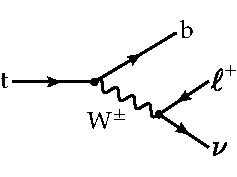
\includegraphics[scale=0.75]{figures/theory/t_decay.pdf}}\hspace{0.15\textwidth}
\subfloat[\label{fig:theory-top-whel-angle}]{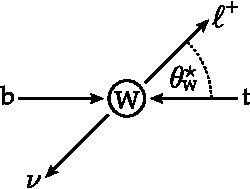
\includegraphics[scale=0.75]{figures/theory/whel.pdf}}
}

Potential scenarios of spin orientations at the $\mathrm{Wtb}$~vertex are presented in Fig.~\ref{fig:theory-top-whel-states} for longitudinal~($H=0$), left-handed~($H=-1$), and right-handed~($H=+1$) $\mathrm{W}$~bosons in the top quark rest frame. In the last scenario the conservation of angular momentum forces the $\mathrm{b}$~quark to be right-handed. This is however suppressed by the electroweak \gls{va} coupling structure leading to a nearly vanishing probability at \gls{lo}. It would vanish entirely only for massless $\mathrm{b}$~quarks since then the $\mathrm{b}$~quark helicity would be equal to its chirality~\cite{Bernreuther:2008ju}. The expected distributions per helicity state as a function of $\cos\theta^\star_\mathrm{W}$ are shown in Fig.~\ref{fig:theory-whel-distributions} together with the \gls{nnlo} \gls{sm} expectation of $\mathrm{F}_\mathrm{L}=0.311\pm0.005$, $\mathrm{F}_\mathrm{R}=0.0017\pm0.0001$, and $\mathrm{F}_{0}=0.687\pm0.005$~\cite{Czarnecki:2010gb}. The non-zero but small right-handed helicity fraction arises from the non-zero mass of the $\mathrm{b}$~quark and from the considered corrections beyond \gls{lo} to the vertices.
 
\myfigure{\label{fig:theory-top-whel-states}Scenarios of spin orientations at the $\mathrm{Wtb}$~vertex in the top quark rest frame. The right-handed $\mathrm{W}$~boson helicity~($H=+1$) is suppressed by the electroweak \gls{va} coupling structure which does not allow the right-handed $\mathrm{b}$~quark~(marked in red) to interact.}{
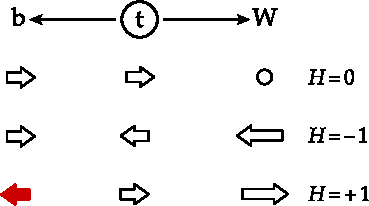
\includegraphics[scale=0.75]{figures/theory/whel_spins.pdf}
}
 
\myfigure{\label{fig:theory-whel-distributions}Distributions of the helicity angle for various W boson helicity scenarios. The \gls{sm} expectation at \gls{nnlo} is taken from Ref.~\cite{Czarnecki:2010gb}.}{
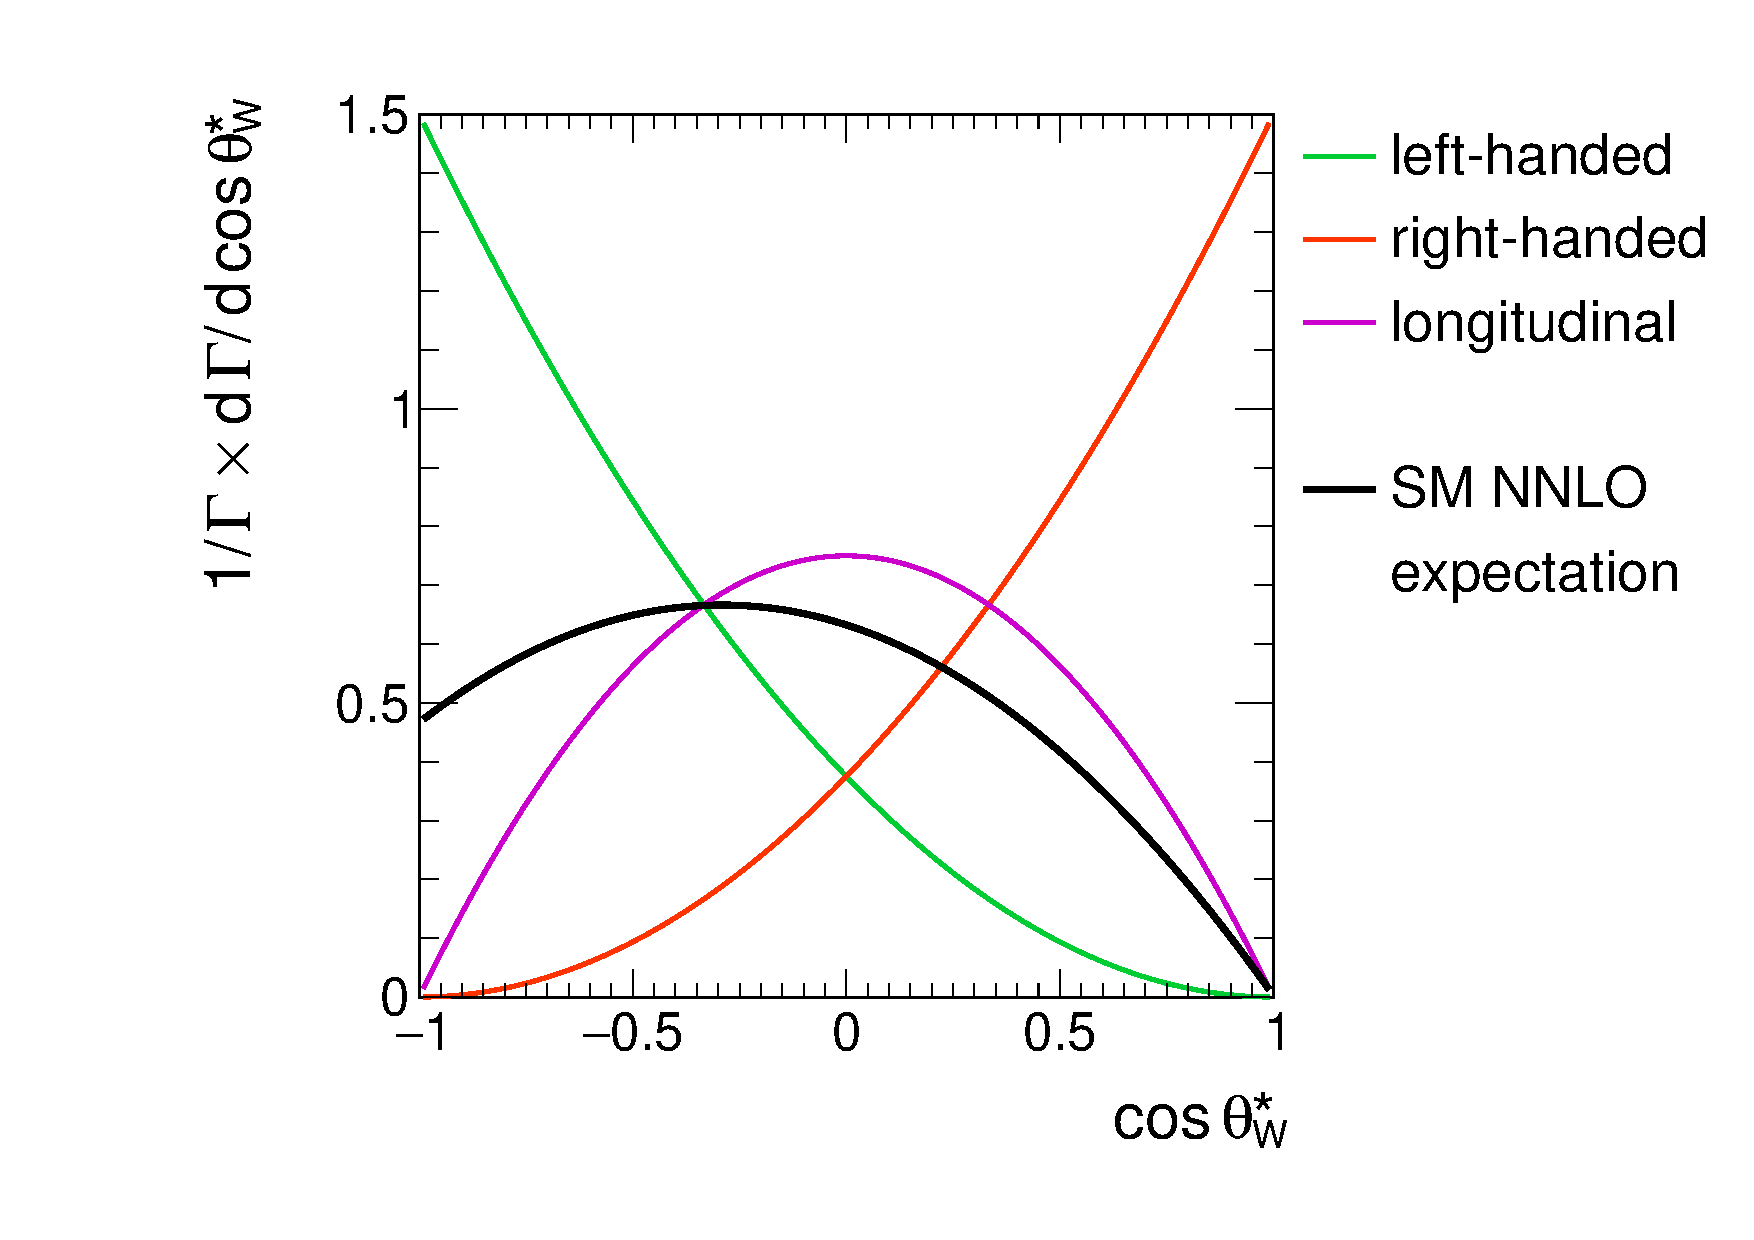
\includegraphics[width=0.49\textwidth]{figures/theory/whel_fractions.pdf}
}

For a general analysis of the top quark spin one introduces the so-called ``spin-analyzing power'', $\alpha_{X}\in[-1;\,1]$, of the decay product $X=\ell,\nu,\mathrm{W},\mathrm{b}$. It denotes the fraction of instances when the top quark spin is aligned along the momentum of the spin analyzer in the top quark rest frame. The calculated spin-analyzing powers at \gls{lo} and \gls{nlo} in the \gls{sm} are listed in Tab.~\ref{tab:theory-spin-powers}. Additionally, the spin-analyzing powers for $X=\mathrm{q},\mathrm{q}^\prime$ for $\mathrm{W}\to \mathrm{q}\,\mathrm{q}^\prime$ decays are provided where $\mathrm{q}$ ($\mathrm{q}^\prime$) denotes all up-type (down-type) quarks respectively. However, studying the top quark spin in those decays is experimentally very challenging since the original quark flavor of a jet and its origin in case of additional final state radiation are difficult to infer. The spin-analyzing powers flip their sign $\alpha_{X}=-\alpha_{\bar{X}}$ in the case of top antiquark decays for the corresponding particle or antiparticle. This holds also in \gls{bsm} scenarios inducing \gls{cp}-violation in the top quark sector~\cite{AguilarSaavedra:2010nx}.

\mytable{\label{tab:theory-spin-powers}Spin-analyzing power of the decay particles of the top quark. The values are taken from Ref.~\cite{AguilarSaavedra:2010nx} and references therein.}{
\begin{tabular}{@{}l  r@{.}l c r@{.}l@{} }
\toprule
Decay product \hspace{0.4cm}          &  \multicolumn{5}{c@{}}{spin-analyzing power} \\
\cmidrule{2-6}
& \multicolumn{2}{c}{\gls{lo}}      && \multicolumn{2}{c}{\gls{nlo}} \\
\midrule
$\ell^{\rmplus}$            & \hspace{0.2cm}1&00\hspace{0.2cm}                  && \hspace{0.3cm}0&998 \\
$\nu$                       & -0&32                     && -0&33 \\
$\bar{\mathrm{q}}^\prime$ (down-type)   & 1&00          && 0&93 \\
$\mathrm{q}$~(up-type)      & -0&32                     && -0&31 \\
$\mathrm{b}$                & -0&41                     && -0&39 \\
$\mathrm{W}^{\rmplus}$      & 0&41                      && 0&39 \\
\bottomrule
\end{tabular}
}

The charged lepton is a nearly perfect spin analyzer to study the top quark polarization. Its spin-analyzing power is even larger than that of its mother particle, the $\mathrm{W}$~boson, due to constructive (destructive) interference of the longitudinal and left-handed $\mathrm{W}$~boson helicity states in cases when the lepton is aligned (antialigned) with the top quark spin, respectively~\cite{Bernreuther:2008ju}. Simplified sketches of various spin orientations for longitudinal and left-handed $\mathrm{W}$~boson helicities are shown in Fig.~\ref{fig:theory-top-spin-orientations} demonstrating that the momentum of the charged antilepton in the top quark rest frame tends to be aligned along the top quark spin. Antialigned scenarios~(Figs.~\ref{fig:theory-top-spin-orientations-long-suppressed} and~\ref{fig:theory-top-spin-orientations-left-suppressed}) are suppressed by the \gls{va} coupling structure which does not allow right-handed particles~($\nu$) or left-handed antiparticles~($\ell^{\rmplus}$) to interact. Similar diagrams with reversed spin orientations are expected for top antiquarks.

\myfigure{\label{fig:theory-top-spin-orientations}Sketches of various spin orientations in top quark decays for (a,b)~longitudinal and (c,d)~left-handed $\mathrm{W}$~boson helicities. Suppressed spin orientations are marked in red.}{
\subfloat[]{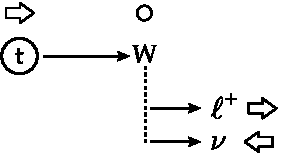
\includegraphics[scale=0.75]{figures/theory/top_spins_long_allowed.pdf}}\hspace{0.15\textwidth}
\subfloat[\label{fig:theory-top-spin-orientations-long-suppressed}]{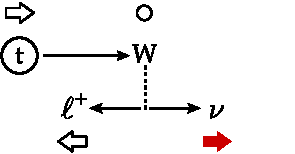
\includegraphics[scale=0.75]{figures/theory/top_spins_long_suppressed.pdf}}\\
\subfloat[]{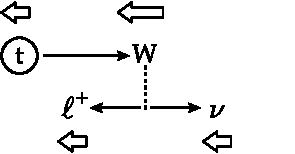
\includegraphics[scale=0.75]{figures/theory/top_spins_left_allowed.pdf}}\hspace{0.15\textwidth}
\subfloat[\label{fig:theory-top-spin-orientations-left-suppressed}]{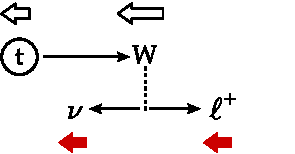
\includegraphics[scale=0.75]{figures/theory/top_spins_left_suppressed.pdf}}
}

%##############################################
\section{Pair production}
%##############################################
\label{sec:theory-ttbar-production}

The dominant mechanism producing top quarks at hadron colliders is top quark pair production through strong interactions via gluon~($gg\to\ttbar$) or quark fusion~($\mathrm{q}\bar{\mathrm{q}}\to\ttbar$). Figure~\ref{fig:theory-feynman-ttbar} shows the contributing Feynman diagrams at \gls{lo}. Especially the production channel via gluon fusion leads to a large cross section at the \gls{lhc} because of the steeply increasing gluon \gls{pdf} towards smaller momentum fractions. This channel contributes approximately $80\range90\%$ to the total cross section in the \gls{lhc} \acrlong{cm} energy regime of $7\range14~\TeV$~\cite{Olive:2016xmw}. The theoretical \ttbar cross sections in pp collisions at \acrlong{cm} energies of $8$ and $13~\TeV$, relevant for this thesis are listed in Tab.~\ref{tab:theory-ttbar-xsecs}. Those have been calculated at \gls{nnlo}+NNLL accuracy using the \textsc{Top++}\,2.0 program~\cite{Czakon:2011xx,Czakon:2013goa} assuming a top quark mass of $172.5~\GeV$. The \gls{pdf} uncertainty includes also the uncertainty on \as.

\myfigure{\label{fig:theory-feynman-ttbar}Feynman diagrams of \ttbar production at \gls{lo}: (a)~quark fusion; (b,c)~gluon fusion.}{
\subfloat[]{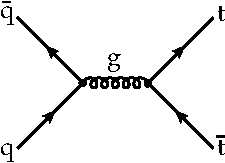
\includegraphics[scale=0.75]{figures/theory/qq2tt_1.pdf}}\hspace{0.03\textwidth}
\subfloat[]{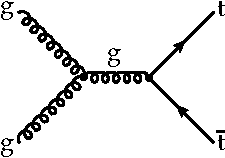
\includegraphics[scale=0.75]{figures/theory/qq2tt_2.pdf}}\hspace{0.03\textwidth}
\subfloat[]{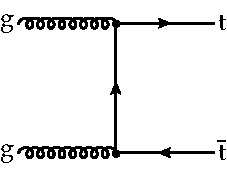
\includegraphics[scale=0.75]{figures/theory/qq2tt_3.pdf}}
}

\mytable{\label{tab:theory-ttbar-xsecs}Top quark pair production cross sections in per \acrlong{cm} energy.}{
\begin{tabular}{@{}l r@{.}l@{}l@{$\,\mathrm{(scale)}$}l@{$\,\mathrm{(\gls{pdf})}~\pb$}l@{} }
\toprule
\gls{cm}~energy \hspace{0.3cm}      & \multicolumn{5}{c }{cross section}     \\
\midrule
$8~\TeV$     & $252$ & $9$ & ${}^{+6.4}_{-8.6}$ & $\pm11.7$ & \\
$13~\TeV$    & $831$ & $8$ & ${}^{+19.8}_{-29.2}$ & $\pm35.6$ & \\
\bottomrule
\end{tabular}
}



%##############################################
\section{Single top quark production}
%##############################################
\label{sec:theory-single-top-production}

Besides the production in pairs, top quarks can be produced singly through electroweak interactions. At \gls{lo}, one can categorized the production into three main channels depending on the exchanged $\mathrm{W}$~boson and its virtuality $Q^{2}=-p_{\mu}p^{\mu}$. The corresponding Feynman diagrams are presented in Fig.~\ref{fig:theory-feynman-singletop}. Overall, the single-top-quark cross sections are smaller than for pair production due to the electroweak coupling strength $\aw<\as$. Additionally, the requirement of sea quarks~($\mathrm{b}$, $\bar{\mathrm{q}}$) in the initial states whose \glspl{pdf} increase less steeply at low momentum fractions compared to the gluon \gls{pdf} suppresses the cross sections further~(see Fig.~\ref{fig:theory-nnpdf-dist}).

\myfigure{\label{fig:theory-feynman-singletop}Feynman diagrams of electroweak single-top-quark production at \gls{lo} in the 5 flavor scheme.}{
\subfloat[\label{fig:theory-singletop-tch}$t$ channel]{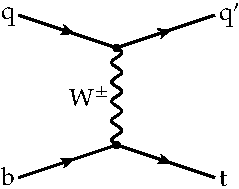
\includegraphics[scale=0.75]{figures/theory/ST_tch.pdf}}\hspace{0.05\textwidth}
\subfloat[\label{fig:theory-singletop-sch}$s$ channel]{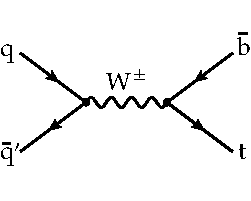
\includegraphics[scale=0.75]{figures/theory/ST_sch.pdf}} \\
\subfloat[\label{fig:theory-singletop-tWch}tW channel]{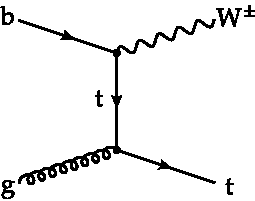
\includegraphics[scale=0.75]{figures/theory/ST_tWch2.pdf}\hspace{0.05\textwidth}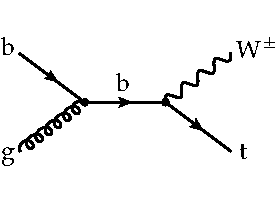
\includegraphics[scale=0.75]{figures/theory/ST_tWch.pdf}}
}

\begin{description}
\item[$\boldsymbol{t}$ channel] The production of single top quarks in $t$-channel~(Fig.~\ref{fig:theory-singletop-tch}) has the highest cross section in $\mathrm{pp}$ collisions. Here, the virtuality of the $\mathrm{W}$~boson is found to be $Q^2>0$ and hence it is said to be ``space-like''. A characteristic feature of this mode is the additional spectator quark $q^\prime$ which recoils against the $\mathrm{W}$~boson and tends therefore being scattered fairly forward. In $t$-channel production, top quarks are produced roughly twice more often than top antiquarks reflecting the u~over d~valence quark ratio of the proton. This ratio depends however on the \acrlong{cm} energy. At higher energies, lower momentum fractions are reached at which the contributions from the valence quarks become less dominant. Hence the $\sigma(\mathrm{t})/\sigma(\bar{\mathrm{t}})$ charge ratio is sensitive to the \gls{pdf} of the proton.
\item[$\boldsymbol{s}$ channel] The mode with the smallest single-top-quark production cross section is via $s$ channel~(Fig.~\ref{fig:theory-singletop-sch}). This is because of the ``time-like'' $\mathrm{W}$~boson which has to have a large virtuality $Q^2<0$ to produce the heavier top quark. In various \gls{bsm} scenarios, the cross section of this process is expected to increase due to new heavy particles such as $\mathrm{W}^\prime$ or charged Higgs bosons which may even be produced on their mass shell, $p_{\mu}p^{\mu}-m^{2}=0$, and hence occur as a resonance.
\item[tW] The third mode is the production of a single top quarks in association with a $\mathrm{W}$~boson~(Fig.~\ref{fig:theory-singletop-tWch}). Here, the $\mathrm{W}$~boson can be produced on-shell $Q^2=-m_\mathrm{W}^{2}$. It is commonly referred to as ``tW channel''. This process interferes at \gls{nlo} with \ttbar production which complicates its definition. In the \glshere{dr} scheme  diagrams with two resonant top quarks are subtracted from the amplitude whereas in the \glshere{ds} scheme the contribution from \ttbar is locally removed from the cross section~\cite{Tait:1999cf,1126-6708-2009-11-074}. The difference between both schemes lies in the treatment of the interference term which is kept in \gls{ds} but removed in \gls{dr}. A new approach is to combine both production modes and the inference between them into a process with a $\mathrm{W}^{\rmplus}\mathrm{W}^{\rmminus}\,\mathrm{b}\,\bar{\mathrm{b}}+X$ final state~\cite{Cascioli:2013wga} whose simulation is currently being studied.
\end{description}

The theoretical cross sections of the three single-top-quark production modes in pp collisions for center-of-mass energies of $8$ and $13~\TeV$, relevant for this thesis, are listed in Tab.~\ref{tab:theory-singletop-xsecs}. These have been calculated at \gls{nlo} in \gls{qcd} with the \HATHOR\,$2.1$ program~\cite{Aliev:2010zk,Kant:2014oha} using a top quark mass of $m_\mathrm{t}=172.5~\GeV$ while setting the factorization and renormalization scales to $\mu_\mathrm{R}=\mu_\mathrm{F}=m_\mathrm{t}$. The \gls{pdf} uncertainty includes also the uncertainty on \as.

\mytable{\label{tab:theory-singletop-xsecs}Single top quark cross sections per production mode and per \acrlong{cm} energy.}{
\begin{tabular}{@{}l r@{.}l@{}l@{$\,\mathrm{(scale)}$}l@{$\,\mathrm{(\gls{pdf})}~\pb$}l  r@{.}l@{}l@{$\,\mathrm{(scale)}$}l@{$\,\mathrm{(\gls{pdf})}~\pb$}l@{}}
\toprule
Mode & \multicolumn{5}{c }{$\sigma^{8~\TeV}$} & \multicolumn{5}{c }{$\sigma^{13~\TeV}$}     \\
\midrule
$t$ channel     & $84$ & $7$ & ${}^{+2.6}_{-1.7}$ & $\pm2.8$ &   \hspace{0.15cm}   & $217$ & $0$ & ${}^{+6.6}_{-4.6}$ & $\pm6.2$ & \\
tW channel      & $22$ & $4$ & $\pm0.6$ & $\pm1.4$ &      & $71$  & $7$ & $\pm1.8$ & $\pm3.4$ & \\
$s$ channel     & $5$  & $24$ & ${}^{+0.15}_{-0.12}$ & $\pm0.16$ &      & $10$  & $32$ & ${}^{+0.29}_{-0.24}$ & $\pm0.27$ & \\
\bottomrule
\end{tabular}
}

Measurements of single-top-quark cross sections allow to extract a limit on the \gls{ckm} matrix element $\vtb$. If one assumes $|\vtd|^2+|\vts|^2\ll|\vtb|^2$ then the $\mathrm{t}\to\mathrm{bW}$ branching ratio can be approximated as

\begin{equation}
\mathcal{B}(\mathrm{t}\to\mathrm{bW})=\frac{|\vtb|^2}{\underbrace{|\vtd|^2+|\vts|^2}_{\ll|\vtb|^2}+|\vtb|^2}\approx 100\%\,.
\end{equation}

Hence, the cross section is independent of the top quark decay vertex and therefore directly proportional to $|f_\mathrm{L}\cdot\vtb|^2$. The form factor $f_\mathrm{L}$ is introduced to absorb potential contributions from \gls{bsm} physics that modify the left-handed coupling strength. It is $f_\mathrm{L}^\mathrm{SM}=1$ in the \gls{sm}. A measured single-top-quark cross section can then be used to extract the value of $|f_\mathrm{L}\vtb|$ as

\begin{equation}
|f_\mathrm{L}\vtb|=\sqrt{\frac{\sigma_\mathrm{measured}}{\sigma_\mathrm{theory}}}\,.
\end{equation}

It should be noted that for this interpretation of single-top-quark cross sections, no assumptions on the number of quark generations and subsequently no unitarity of the \gls{ckm} matrix is required.



%##############################################
\section{Polarization in \textit{t}-channel single-top-quark production}
%##############################################
\label{sec:theory-t-channel-polarization}

The \gls{sm} predicts that top quarks are produced highly polarized in $t$~channel since there are only electroweak interactions with a \gls{va} coupling structure involved at \gls{lo}~\cite{Bernreuther:2008ju}. A new \gls{bsm} physics model may however lead to a depolarization by altering the coupling structure effectively through new production vertices and/or higher order corrections. The differential cross section can be parametrized as

\begin{equation}
\frac{\mathrm{d}\sigma}{\sigma\cdot\mathrm{d}\cos\theta^\star_{X}}=\frac{1}{2}\,\Big(1+\mathrm{P}_\mathrm{t}\cdot\alpha_{X}\cdot\cos\theta^\star_{X}\Big)\,,
\end{equation}

where $\mathrm{P}_\mathrm{t}$ denotes the polarization along a given axis and $\alpha_{X}$ the spin-analyzing power with respect to decay product $X$. The polarization angle

\begin{equation}
\cos\theta^\star_{X}=\frac{\vec{s}_\mathrm{t}\cdot \vec{p}_{X}^\scriptn{\mathrm{(t)}}}{\big|\vec{s}_\mathrm{t}\big|\cdot\big|\vec{p}_{X}^\scriptn{\mathrm{(t)}}\big|}
\end{equation}

is taken between the spin analyzer $X$ in the top quark rest frame and a suitable spin quantization axis $\vec{s}_\mathrm{t}$. A potential spin axis is given in the helicity basis where the top quark momentum in the partonic \acrlong{cm} system is chosen, $\vec{s}_\mathrm{t}^\scriptn{\,\mathrm{hel.}}=\vec{p}_\mathrm{t}^\scriptn{\mathrm{(tq)}}$. However, this system cannot be reconstructed unambiguously beyond \gls{lo} when additional \glshere{isr} or \glshere{fsr} occurs. An alternative axis is motivated in Fig.~\ref{fig:theory-t-channel-prod-decay} where a sketch of spin orientations in the top quark rest frame for $t$-channel production and decay is shown. There exists a symmetry between a down-type spectator quark on the production side and the charged antilepton on the decay side leading to a correlation between their momentum directions and the intermediate top quark spin. This suggests to take the spectator quark momentum in the top quark rest frame as the spin quantization axis, $\vec{s}_\mathrm{t}=\vec{p}_{\mathrm{q}^\prime}^\scriptn{\mathrm{(t)}}$. At \gls{lo}, this axis would coincide with the axis in helicity basis since the top quark and the spectator quark are back-to-back in the \acrlong{cm} system~\cite{Schwienhorst:2010je}. A high degree of polarization can therefore be expected. This is further motivated by the fact that the charged lepton is a nearly perfect spin analyzer and thus the down-type spectator quark is a good spin analyzer as well because of the depicted symmetry. Higher-order corrections however dilute this symmetry somewhat as also expected from Tab.~\ref{tab:theory-spin-powers} where a slightly lower spin-analyzing power for the down-type quark compared to the charge lepton at \gls{nlo} is expected. 

\myfigure{\label{fig:theory-t-channel-prod-decay}Sketch of spin orientations in $t$-channel single-top-quark production and decay. The figure has been inspired from Ref.~\cite{Schwienhorst:2010je}.}{
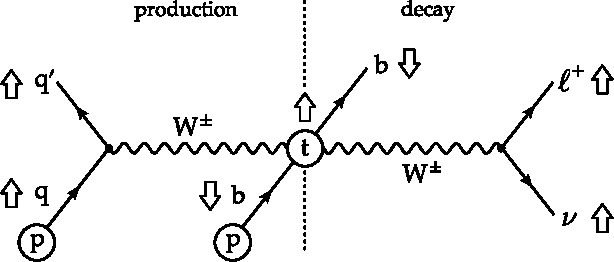
\includegraphics[scale=0.75]{figures/theory/t-channel-prod-decay.pdf}
}

A crucial ingredient which is still missing in this argumentation is the fact that the spectator quark has to be of down-type flavor. This is only true in about $80\%$ for $t$-channel top quark production but only in $31\%$ of all cases for top antiquark production. Here, the down-type quark is found with a probability of $69\%$ in the initial state instead. However, the spectator quark is only mildly deflected after recoiling against the $\mathrm{W}$~boson. It is therefore still sufficiently close to the direction of the down-type quark momentum resulting in a high degree of polarization nonetheless~\cite{Bernreuther:2008ju}.

The expect top quark polarizations have been calculated at $7~\TeV$ and are listed in Tab.~\ref{tab:theory-singletop-sm-polarization} at \gls{lo} and \gls{nlo}. The combined polarization for top quark and antiquark is calculated using a weighted sum with the corresponding cross sections as weights\footnote{The expected single-top-quark cross sections at $7~\TeV$ are $\sigma(\mathrm{t})=41.8^{+1.8}_{-1.5}~\pb$ and $\sigma(\bar{\mathrm{t}})=22.0^{+1.3}_{-1.2}~\pb$. These are calculated with the same setup as used for Tab.~\ref{tab:theory-singletop-xsecs}}. At $8~\TeV$, a similar polarization of $|\mathrm{P}_{\mathrm{t}+\bar{\mathrm{t}}}^\mathrm{8~\TeV}|=0.88$ is expected using simulated events from the \gls{nlo} generator \textsc{Powheg}~\cite{Khachatryan:2015dzz}.

\mytable{\label{tab:theory-singletop-sm-polarization}Expected polarizations of top quarks and top antiquarks in $t$-channel single-top-quark production at $7~\TeV$. The values are taken from Ref.~\cite{Schwienhorst:2010je}.}{
\begin{tabular}{@{}l r@{.}l r@{.}l r@{.}l@{}}
\toprule
            & \multicolumn{2}{c}{$\mathrm{P}_\mathrm{t}^\mathrm{\,7\,\TeV}$} & \multicolumn{2}{c}{$\mathrm{P}_{\bar{\mathrm{t}}}^\mathrm{\,7\,\TeV}$} & \multicolumn{2}{c}{$|\mathrm{P}_{\mathrm{t}+\bar{\mathrm{t}}}^\mathrm{\,7\,\TeV}|$}     \\
\midrule
\gls{lo}    & \hspace{0.5cm}0&99\hspace{0.5cm} & \hspace{0.5cm}-0&93\hspace{0.5cm}       & \hspace{0.5cm}0&95\hspace{0.5cm}          \\
\gls{nlo}   & 0&91                             & -0&86                                   & 0&88          \\
\bottomrule
\end{tabular}
}

The high polarization of the top quark along the spectator quark momentum allows also to extend the $\mathrm{W}$~boson polarization with two additional axes. Figure~\ref{fig:theory-ext-whel} shows the construction procedure. The top quark spin is approximated by the spectator quark momentum. Then the normal and transverse axes are defined as 

\begin{subequations}
\begin{align}
\vec{\mathrm{N}}&=\vec{p}_{\mathrm{q}^\prime}^{\mathrm{(t)}}\times\vec{p}_{\mathrm{W}}^{\mathrm{(t)}}\qquad\text{(normal axis)} \\
\vec{\mathrm{T}}&=\vec{p}_{\mathrm{W}}^{\mathrm{(t)}}\times \vec{\mathrm{N}}\qquad\text{(transverse axis)}.
\end{align}
\end{subequations}

\myfigure{\label{fig:theory-ext-whel}Extended $\mathrm{W}$~boson polarization axes in $t$-channel single-top-quark production and decay: $\mathrm{N}=\text{normal axis}$; $\mathrm{T}=\text{transverse axis}$.}{
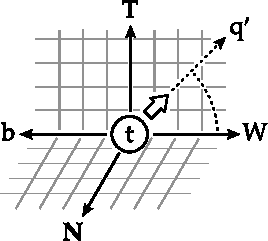
\includegraphics[scale=0.75]{figures/theory/ext_whel.pdf}
}

The differential cross section as a function of the polarization angles with these new axes takes the same functional form as in Eq.~\ref{eq:theory-diff-whel-fractions}. However, the corresponding polarization fractions $\mathrm{F}_\mathrm{L}^\mathrm{N,T}$, $\mathrm{F}_\mathrm{0}^\mathrm{N,T}$, and $\mathrm{F}_\mathrm{R}^\mathrm{N,T}$ are probing here different aspects of the coupling structure. In particular, the left- and right-handed polarization along $\vec{\mathrm{N}}$ are sensitive to potential \gls{cp}-violation~\cite{AguilarSaavedra:2010nx}. Since the top quark is not fully polarized along the spectator quark momentum, the  polarization fractions are modified as

\begin{subequations}
\begin{align}
\tilde{\mathrm{F}}_\mathrm{R}^\mathrm{N,T}&=\frac{1+\mathrm{P}_\mathrm{t}}{2}\cdot\mathrm{F}_\mathrm{R}^\mathrm{N,T}+\frac{1-\mathrm{P}_\mathrm{t}}{2}\cdot\mathrm{F}_\mathrm{L}^\mathrm{N,T}, \\
\tilde{\mathrm{F}}_\mathrm{L}^\mathrm{N,T}&=\frac{1+\mathrm{P}_\mathrm{t}}{2}\cdot\mathrm{F}_\mathrm{L}^\mathrm{N,T}+\frac{1-\mathrm{P}_\mathrm{t}}{2}\cdot\mathrm{F}_\mathrm{R}^\mathrm{N,T}, \\
\tilde{\mathrm{F}}_\mathrm{0}^\mathrm{N,T}&=\mathrm{F}_\mathrm{0}^\mathrm{N,T}\,.
\end{align}
\end{subequations}


%##############################################
\section{Flavor schemes}
%##############################################
\label{sec:theory-flavor-schemes}

In single-top-quark production via $t$ channel, a $\mathrm{b}$~quark is required in the initial state. There are two different ways called 4 and 5~\glshere{fs} to treat the $\mathrm{b}$~quark in theoretical calculations. They differ in the number of quark flavors which are included within the proton~\gls{pdf}. Figure~\ref{fig:theory-flavorscheme} shows a representative Feynam diagram where in 4~\gls{fs} the $\mathrm{b}$~quark originates from gluon splitting and is not part of the \gls{pdf}. In 5~\gls{fs} this splitting is resumed into the \gls{pdf} instead.

\myfigure{\label{fig:theory-flavorscheme}Feynman diagram at \gls{lo} for $t$-channel single-top-quark production in 4 and 5~\glsreset{fs}\gls{fs}. The dashed lines denote where the partonic initial state begins.}{
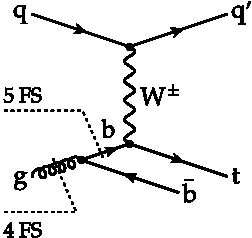
\includegraphics[scale=0.75]{figures/theory/flavorscheme.pdf}
}

Since the $\mathrm{b}$~quark mass of $m_\mathrm{b}\approx4.2~\GeV$ is higher than the mass of the proton, $m_\mathrm{p}\approx1~\GeV$, the 4~\gls{fs} seems more natural at first glance. The $\mathrm{b}$~quark is treated as a heavy quark state that decouples completely from the \as and \gls{pdf} evolutions through renormalization and the DGLAP equation, respectively. However, this approach results in terms proportional to $\log(Q^2/m_\mathrm{b}^2)$ arising from the intermediate $\mathrm{b}$~quark propagator which may prohibit the convergence of perturbative calculations at high momentum transfers $Q$. In this case, such terms together with the $g\to\mathrm{b}\bar{\mathrm{b}}$ splitting function can be absorbed into a \gls{pdf} for the $\mathrm{b}$~quark instead~\cite{Maltoni:2012pa}.

Both schemes are valid approaches for calculating observables. The difference at fixed order stems from the energy scale at which a process is described. Both approaches will converge at sufficiently high orders. This is demonstrated in Fig.~\ref{fig:theory-t-channel-xsec-fs} where the $t$-channel single-top-quark cross section at $14~\TeV$ as a function of the renormalization and factorization scale is depicted. The dashed curves show the \gls{lo} predictions in 4~and 5~\gls{fs} respectively which are far apart. Their opposite behavior originates from the running of coupling constant \as in the 4~\gls{fs} versus the scale dependence of the $\mathrm{b}$~quark \gls{pdf} in the 5~\gls{fs}~\cite{Maltoni:2012pa}. They approach the \gls{nlo} prediction only at low (large) scales for 4~\gls{fs} (5~\gls{fs}) respectively. On the other hand, the \gls{nlo} predictions start to converge already at a scale choice of $\mu\approx m_\mathrm{t}/2$ for this process.

\myfigure{\label{fig:theory-t-channel-xsec-fs}Single-top-quark cross section in $t$ channel for top quarks at $14~\TeV$ as a function of the renormalization and factorization scale $\kappa=\mu/m_\mathrm{t}$. The predicted cross sections calculated in 4~and 5~\gls{fs} at \gls{lo} and \gls{nlo} are displayed. The figure is taken from Ref.~\cite{Maltoni:2012pa}}{
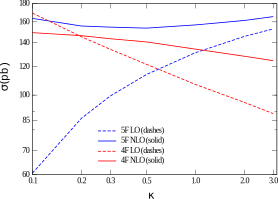
\includegraphics[scale=0.9]{figures/theory/t-channel-xsec-fs}
}

Predictions of differential distributions are also affected by the flavor scheme choice. Ratios of 4~\gls{fs} over 5~\gls{fs} differential $t$-channel cross sections at \gls{nlo} as a function of the transverse momentum and pseudo rapidity with respect to the top quark and spectator jet are shown in Fig.~\ref{fig:theory-t-channel-xsec-fs-diff}. The differences between both schemes are found to be around the $10~\%$ level~\cite{Campbell:2009ss}. In particular, the top quark \pt displays here an almost linear increasing ratio.

\myfigure{\label{fig:theory-t-channel-xsec-fs-diff}Ratio of 4~\gls{fs}~($\sigma^{2\to3}$) over 5~\gls{fs}~($\sigma^{2\to2}$) differential single-top-quark cross sections in $t$ channel for top quarks at $14~\TeV$ as a function of (a)~the transverse momentum and (b)~the pseudo rapidity of the top quark and light (spectator) jet. The figures are taken from Ref.~\cite{Campbell:2009ss}}{
\subfloat[]{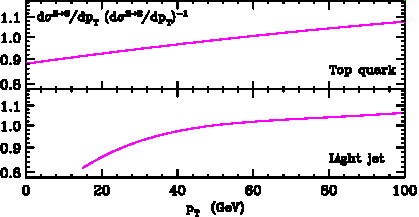
\includegraphics[scale=1]{figures/theory/t-channel-fs-diff-pt.pdf}}\\
\subfloat[]{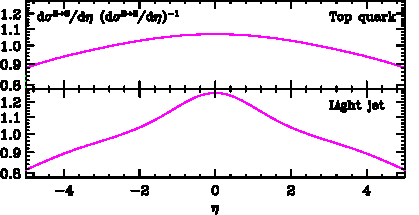
\includegraphics[scale=1]{figures/theory/t-channel-fs-diff-eta.pdf}}
}


%##############################################
\section{Anomalous couplings}
%##############################################
\label{sec:theory-anomalous-couplings}

Direct searches for \gls{bsm} physics can be viewed as a top-down approach. The starting point is marked by a well-defined and usually \gls{uv}-complete \gls{bsm} theory. Experimentally, one is then interested to detect additional events originating from a new process within such a theory. Exemplary models are the \glshere{mssm}~(reviewed in Ref.~\cite{Csaki:1996ks}) or the \glshere{2hdm}~\cite{Branco:2011iw}. Since no signal has been found yet it may be that the energy scale at which a \gls{bsm} process becomes significant is not accessible in direct searches. Nonetheless, new particles or interactions can contribute higher-order corrections to processes within the \gls{sm} already at low energies. An example is the observation of the rare $\mathrm{B}^{0}_\mathrm{s}\to\mu\mu$ decay~\cite{CMS:2014xfa} which can be altered by contributions from e.g. the \gls{mssm}. This motivates a model-independent bottom-up approach where observables of the \gls{sm} are measured with great precision and compared to their expectation. Any deviations can then be interpreted within multiple new theories.

The idea of a bottom-up approach is depicted in Fig.~\ref{fig:theory-t-channel-eff} for some exemplary \gls{uv}-complete theory contributing to single-top-quark production through a new heavy scalar particle $\chi$. If the new particle has a sufficiently high mass it would not be possible to observe it as a new resonance in $s$~channel. However, the shown production of single top quarks would be altered through additional contributions from this new process. At energies $q\ll m_{\chi}$ it would mimic a 4-fermion contact interaction with a simple scalar coupling structure. The \mbox{\gls{sm}+\gls{bsm}} cross section of this process may still correspond to the one expected from the \gls{sm} alone by fine-tuning the \gls{sm} and \gls{bsm} couplings correspondingly. However, since this new process has a scalar coupling structure it manifests itself as a deviation from the expected \gls{va} coupling structure. Differential cross section measurements and related observables like the top quark polarization can then be used to probe for such anomalous couplings at the production vertex.

\myfigure{\label{fig:theory-t-channel-eff}Feynman diagram of potential \gls{bsm} physics contributing to single-top-quark production via flavor-changing neutral current interaction. At low energies $p\ll m_\chi$ the propagator in (a) can be approximated as an anomalous 4-fermion coupling~(b).}{
\subfloat[\label{fig:theory-t-channel-chi-uv}$t$~channel]{\parbox{0.35\textwidth}{\centering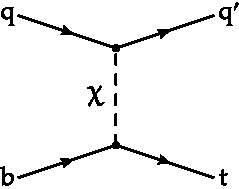
\includegraphics[scale=0.75]{figures/theory/t-channel-chi.pdf}\\$\propto \frac{g^2}{p^2-m^{2}_{\chi}}$}}
\subfloat[\label{fig:theory-t-channel-eff-ir}effective interaction]{\parbox{0.35\textwidth}{\centering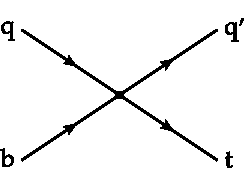
\includegraphics[scale=0.75]{figures/theory/t-channel-contact.pdf}\\$\propto \frac{g^2}{m^{2}_{\chi}}$}}
}

Such deviations from the \gls{sm} coupling structure can be characterized in the framework of effective field theories~(\glsplmark{eft}) in a model-independent manner. Those can be derived using an \glshere{ope} as first proposed in Ref.~\cite{Wilson:1972ee}. Here, products of operators are expanded as

\begin{equation}
{O}_{1}(x_{1})\ldots {O}_{n}(x_{n})=\sum_{i}c_{1\ldots n}^{i}(x_{1},\ldots x_{n})\cdot{O}_{i}^\mathrm{eff}(x_{n})\,,
\end{equation}

where $O_{i}^\mathrm{eff}$ denote effective operators and $c^{i}$ are the so-called Wilson coefficients. The expansion is applicable if $x_{1\ldots n-1}$ are close to $x_n$, i.e. only the low energy limit of a \gls{uv}-complete theory is relevant. Otherwise, unitarity can be violate if the energy scale of a process within the \gls{eft} approaches the scale of the concrete \gls{bsm} theory as discussed in Sec.~\ref{sec:theory-observables}. In the example above this would be the case when the momentum transfer $q$ approaches $m_\chi$. Here, the \gls{eft} approach becomes invalid.

One can extend the Lagrangian of the \gls{sm}, which contains only operators up to dimension-four, into an effective one as

\begin{equation}
\mathcal{L}^\mathrm{eff}=\mathcal{L}^\mathrm{\gls{sm}}_\mathrm{(4)}+\frac{1}{\Lambda}\sum_{i}c_{i}^\mathrm{(5)}{O}_{i}^\mathrm{(5)}+\frac{1}{\Lambda^{2}}\sum_{i}c_{i}^\mathrm{(6)}{O}_{i}^\mathrm{(6)}+\mathcal{O}\left(\frac{O^\mathrm{(7)}}{\Lambda^3}\right)\,,
\end{equation}

where new effective operators of dimension-five and -six have been added. Those are however suppressed by inverse powers of the new physics scale $\Lambda$. This approach leads to 59 independent operators of dimension-six when requiring gauge invariance and baryon number conservation~\cite{Grzadkowski:2010es}. The only operator of dimension-five is

\begin{equation}
\mathcal{L}^\mathrm{eff.}_\mathrm{(5)}=\frac{1}{\Lambda}c^{ij}_{\nu\nu}\Big({\mathrm{E}}^{c}_{\mathrm{L},i}\tilde{\phi}\Big)^\mathrm{T}\Big(\vec{\mathrm{E}}_{\mathrm{L},j}\tilde{\phi}\Big)+\mathrm{\gls{hc}},\qquad \tilde{\phi}_{a}=\epsilon_{ab}\phi_{b}
\end{equation}

which can be used to introduce neutrino masses and mixing after electroweak symmetry breaking\footnote{This assumes Majorana neutrinos. The coefficients $c^{ij}(v^2/\Lambda)$ can be interpreted as mass mixing matrix for neutrinos similar to the \gls{ckm} matrix for quarks. The superscript $c$ stands for charge conjugation.}. Only a subset of operators are relevant in the top quark sector~\cite{AguilarSaavedra:2008zc}. In particular, the following operators contribute to the $\mathrm{Wtb}$~vertex


\begin{subequations}\label{eq:theory-eft-lagrangian-operators}
\begin{align}
\mathcal{L}^\mathrm{eff.}_\mathrm{Wtb}&=\mathcal{L}^\mathrm{SM}_\mathrm{Wtb}+\frac{1}{\Lambda^2}\Big(c_{\phi\mathrm{q}}^{33}O_{\phi\mathrm{q}}^{33}+c_{\phi\phi}^{33}O_{\phi\phi}^{33}+c_{\mathrm{dW}}^{33}O_{\mathrm{dW}}^{33}+c_{\mathrm{uW}}^{33}O_{\mathrm{uW}}\Big)+\mathrm{\gls{hc}} \\ 
O_{\phi\mathrm{q}}^{33}&=i\Big(\phi^\dagger\omega_{a}\mathrm{D}_\mu\phi\Big)\Big(\bar{\mathrm{Q}}_\mathrm{L}^{3}\gamma^{\mu}\omega^{a}\mathrm{Q}_\mathrm{L}^{3}\Big)\,,\qquad
O_{\phi\phi}^{33}=i\Big(\tilde{\phi}^\dagger\mathrm{D}_\mu\phi\Big)\Big(\bar{\mathrm{u}}_\mathrm{R}^{3}\gamma^{\mu}\mathrm{d}_\mathrm{R}^{3}\Big)\,,\\
O_{\mathrm{dW}}^{33}&=\Big(\bar{\mathrm{Q}}_\mathrm{L}^{3}\sigma^{\mu\nu}\omega_{a}\mathrm{d}_\mathrm{R}^{3}\Big)\phi\,\mathrm{W}^{a}_{\mu\nu}\,,\qquad
O_{\mathrm{uW}}=\Big(\bar{\mathrm{Q}}_\mathrm{L}^{3}\sigma^{\mu\nu}\omega_{a}\mathrm{u}_\mathrm{R}^{3}\Big)\tilde{\phi}\,\mathrm{W}^{a}_{\mu\nu}\,,
\end{align}
\end{subequations}

where $D_\mu$ denotes the covariant derivative~(Eq.~\ref{eq:theory-phi-codev}) and the quark field indices refer to the third generation following the notation of Eqs.~\ref{eq:theory-su2-doublets} and~\ref{eq:theory-su2-singlets}. Anomalous couplings can be introduced after electroweak symmetry breaking which absorb all constant terms including $c_{i}(v^2/\Lambda^2)$. One obtains

\begin{align}
\mathcal{L}^\mathrm{eff.}_\mathrm{Wtb}=&-\frac{g}{\sqrt{2}}\bar{\mathrm{b}}\gamma^{\mu}\big(\mathrm{V}_\mathrm{L}\mathrm{P}_\mathrm{L}+\mathrm{V}_\mathrm{R}\mathrm{P}_\mathrm{R}\big)\mathrm{t}\mathrm{W}_\mu^{\rmminus}\nonumber\\
&-\frac{g}{\sqrt{2}}\bar{\mathrm{b}}\frac{i\sigma^{\mu\nu}q_\nu}{m_\mathrm{W}}\big(\mathrm{g}_\mathrm{L}\mathrm{P}_\mathrm{L}+\mathrm{g}_\mathrm{R}\mathrm{P}_\mathrm{R}\big)\mathrm{t}\mathrm{W}_\mu^{\rmminus}+\mathrm{\gls{hc}}\,,\label{eq:theory-wtb-eff-anomcouplings}
\end{align}

where $\mathrm{V}_\mathrm{L,R}$ and $\mathrm{g}_\mathrm{L,R}$ denote the vector- and tensor-like anomalous couplings respectively. In the \gls{sm}~(Eq.~\ref{eq:theory-qqW-int}) there exists only a vector-like, left-handed coupling $\mathrm{V}_\mathrm{L}=\mathrm{V}_\mathrm{tb}$ whereas the other couplings vanish $\mathrm{V}_\mathrm{R}=\mathrm{g}_\mathrm{L}=\mathrm{g}_\mathrm{R}=0$.

The operator $O_\mathrm{qW}^{ij}$ is missing in Eq.~\ref{eq:theory-eft-lagrangian-operators}. Its contribution can be mostly absorbed by the other operators as

\begin{align}
\mathcal{L}_\mathrm{qW}&=\frac{1}{\Lambda^2}c^{ij}_\mathrm{qW}O_\mathrm{qW}^{ij}=\frac{1}{\Lambda^2}c^{ij}_\mathrm{qW}\Big(\bar{\mathrm{Q}}_{\mathrm{L},i}\gamma^{\mu}\omega_{a}D^\nu\mathrm{Q}_{\mathrm{L},j}\Big)\mathrm{W}_{\mu\nu}^{a}+\mathrm{\gls{hc}}\nonumber\\
&\supset\big(\text{terms }\propto\mathcal{L}_\mathrm{Wtb}^\mathrm{eff.}\big)~+~\frac{g\,\mathrm{Re}(c_\mathrm{qW})}{\Lambda^2}\big(\bar{\mathrm{b}}\gamma^{\mu}\mathrm{P}_\mathrm{L}\mathrm{t}\big)\big(\bar{\mathrm{q}}\gamma_\mu\mathrm{P}_\mathrm{L}\mathrm{q}^\prime\big)+\mathrm{\gls{hc}}\,,\label{eq:theory-4q-eff-anomcouplings}
\end{align}

where however a four-fermion contact interaction term remains~\cite{Bach:2012fb}. This interaction cannot contribute to top quark production and decays via a $\mathrm{Wtb}$~vertex directly which is why it is usually left out of Eqs.~\ref{eq:theory-eft-lagrangian-operators} and~\ref{eq:theory-wtb-eff-anomcouplings}. However, the four-fermion vertex should not be neglected when studying in particular single-top-quark production. Here, it can contribute a $\mathrm{udbt}$~vertex (similar to Fig.~\ref{fig:theory-t-channel-eff-ir}) as an addition to the $\mathrm{Wud}\text{+}\mathrm{Wtb}$~vertices which e.g. occur in the production via $t$~channel.

To constrain anomalous couplings from experimental data, various (pseudo) observables are proposed in literature~\cite{AguilarSaavedra:2010nx,Aguilar-Saavedra:2014eqa,Bernreuther:2015yna}. A few of them are the inclusive single-top-quark cross sections, the W~boson helicity fractions~(Sec.~\ref{sec:theory-top-quark-decay}), and the top quark polarization in $t$~channel~(Sec.~\ref{sec:theory-t-channel-polarization}).


%##############################################
\section{Selection of experimental results}
%##############################################
\label{sec:theory-exp-results}

To conclude this chapter, a selection of experimental results in the top quark sector are presented. An overview of inclusive \ttbar cross section measurements at \acrlong{cm} energies of 5, 7, 8, and 13~\TeV are shown in Fig.~\ref{fig:theory-lhc-ttbar-xsec} and compared to the theoretical \gls{nnlo}+\gls{nnll} prediction. Measurements of inclusive single-top-quark production in $t$, tW, and $s$~channel at 7, 8, and 13~\TeV are summarized and compared to the theoretical \gls{nlo} predictions in Fig.~\ref{fig:theory-lhc-st-xsec}. These cross section measurements can be used to determine the absolute value of the \gls{ckm} matrix element $\vtb$ as detailed in Sec.~\ref{sec:theory-single-top-production}. The results are presented in Fig.~\ref{fig:theory-lhc-vtb}. The currently most precise estimation of $\vtb$ stems from a combination of $t$-channel single-top-quark cross section measurements at 7 and 8~\TeV by \gls{cms} resulting in $|f_\mathrm{L}\vtb|=0.998\pm0.038\,\mathrm{(exp)}\pm0.016\,\mathrm{(theo)}$. This yields a limit of $|\vtb|>0.92$ at 95\%~\gls{cl} when assuming $f_\mathrm{L}=1$ and $|\vtb|<1$.


\myfigure[p]{Overview of inclusive (a)~\ttbar and (b)~single-top-quark cross section measurements by the \gls{atlas}~and \gls{cms}~collaborations at various \acrlong{cm} energies. The figures are taken from the TopLHC working group~\cite{toplhc}.}{
\subfloat[\label{fig:theory-lhc-ttbar-xsec}]{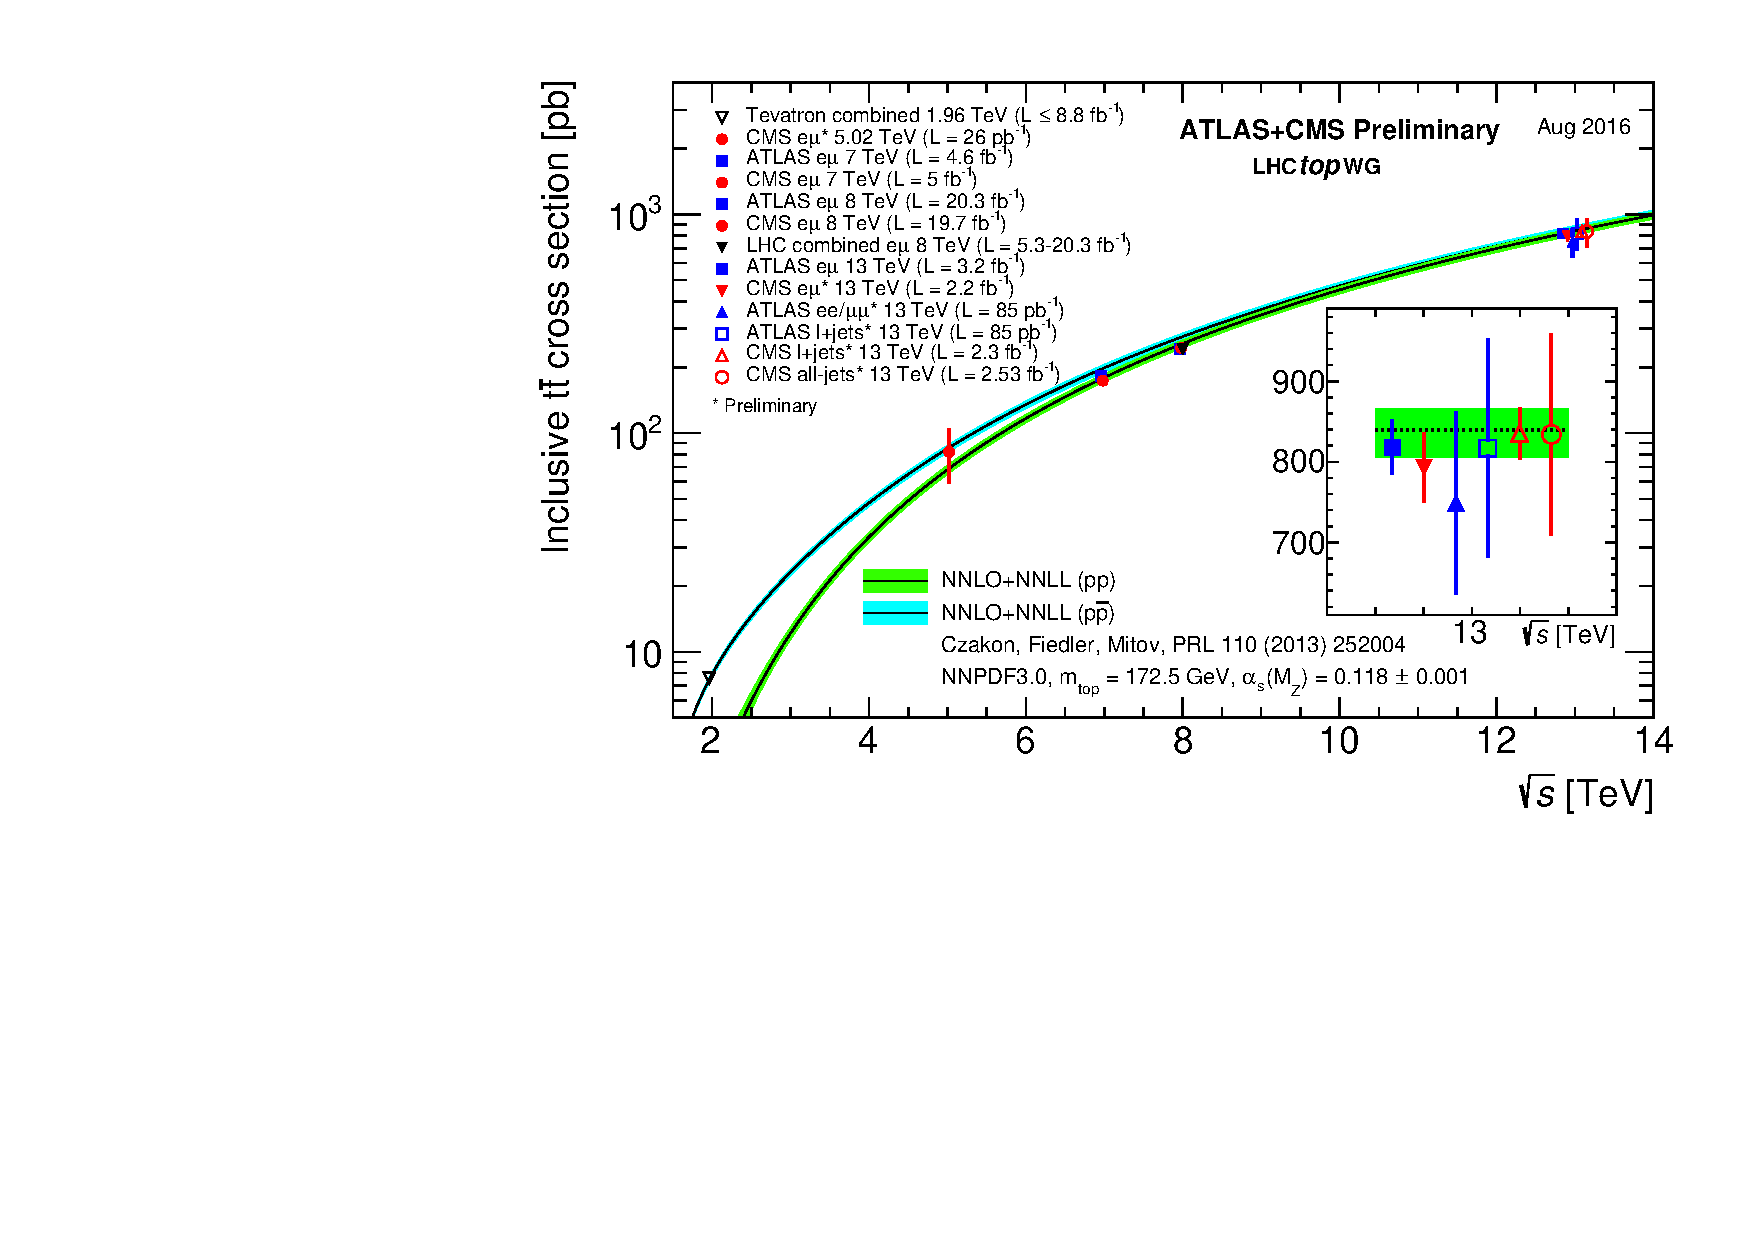
\includegraphics[width=0.96\textwidth]{figures/theory/LHC_ttxsec_sqrts.pdf}}\\
\subfloat[\label{fig:theory-lhc-st-xsec}]{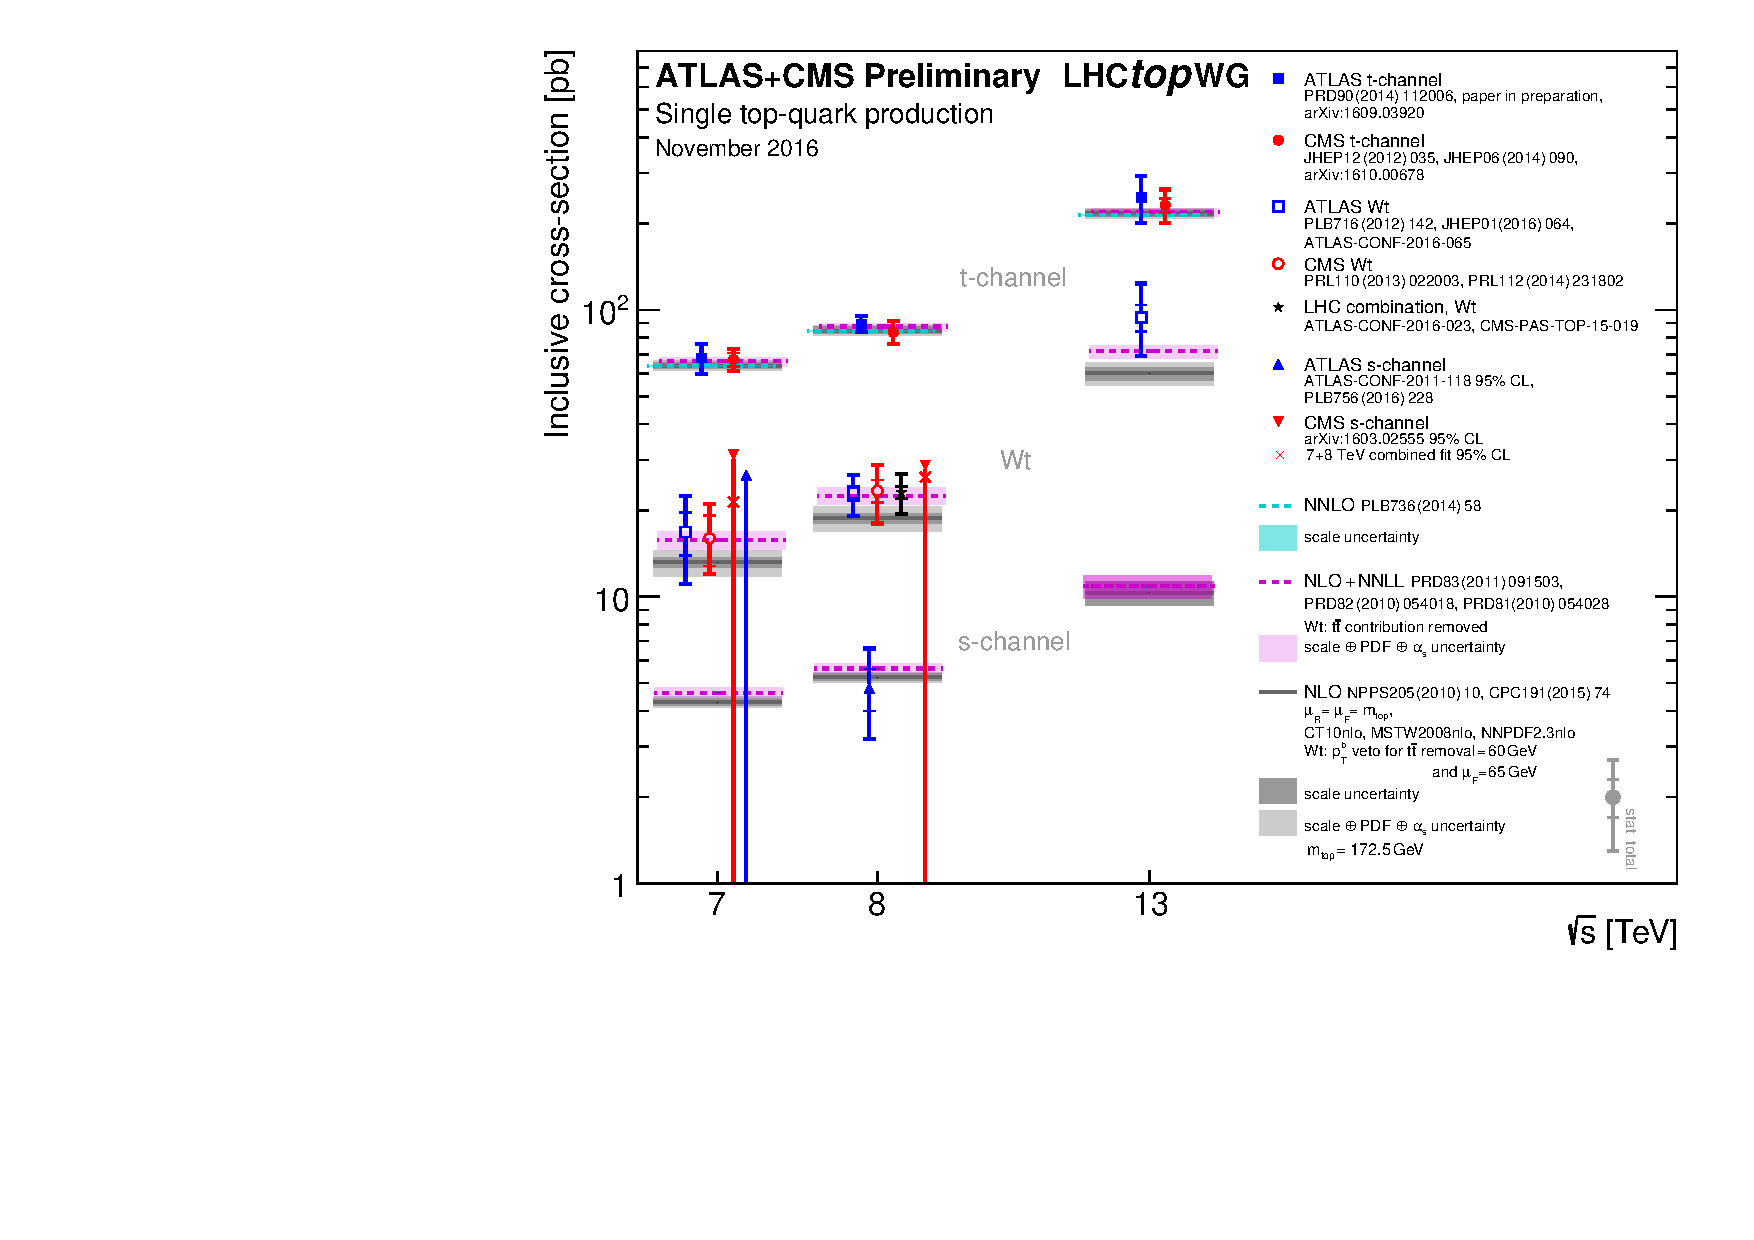
\includegraphics[width=0.9\textwidth]{figures/theory/LHC_singletop_allchannels.pdf}}
}

\myfigure[p]{\label{fig:theory-lhc-vtb}Estimations of the \gls{ckm} matrix element $\vtb$ from single-top-quark cross section measurements. The figure is taken from the TopLHC working group~\cite{toplhc}.}{
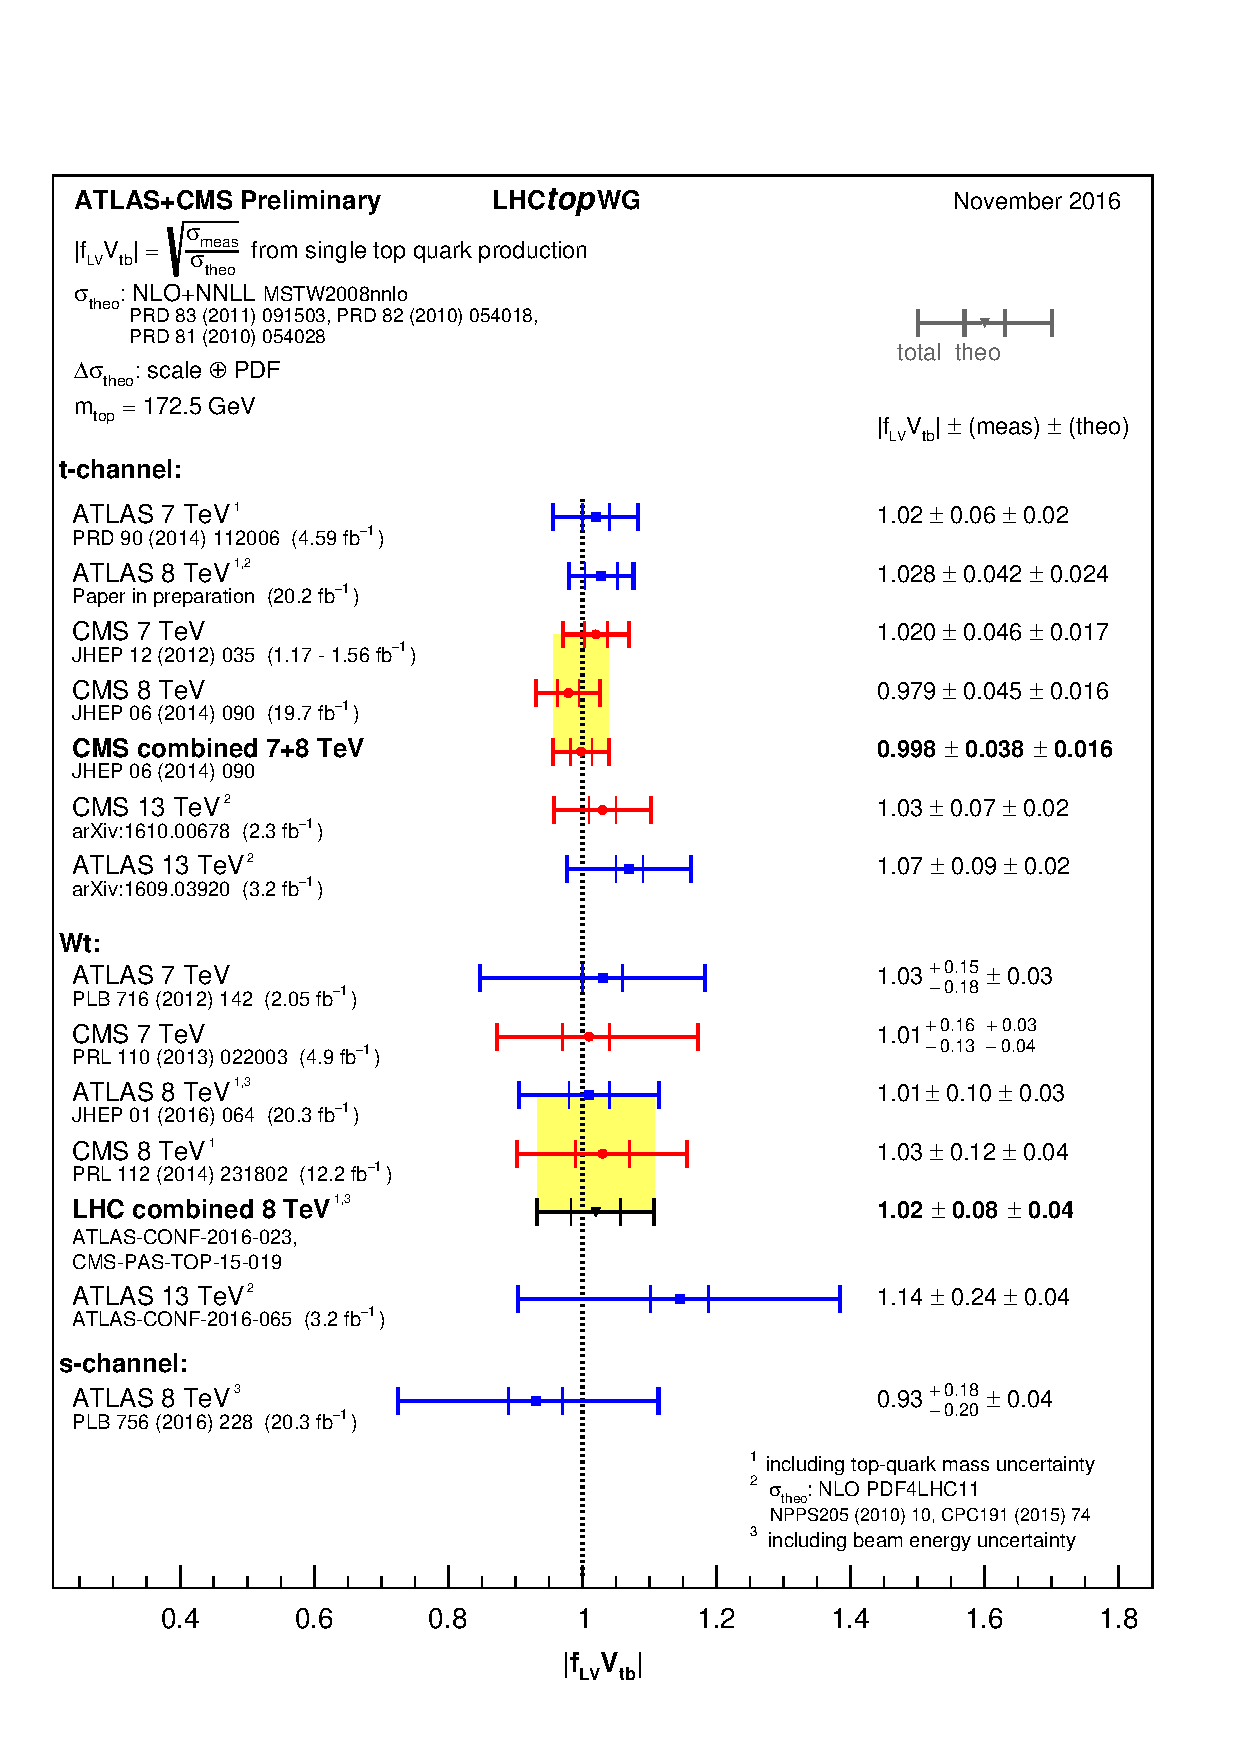
\includegraphics[width=0.99\textwidth]{figures/theory/LHC_singletop_Vtb.pdf}
}

The results from measurements of the $\mathrm{W}$~boson helicity fractions are presented in Fig.~\ref{fig:theory-lhc-whel} and compared to their \gls{nnlo} prediction. These have been mostly obtained by analyzing top quark decays in \ttbar events. However, one measurement used decays of top quarks from $t$-channel single-top-quark production yielding a comparable precision despite the lower production cross section~\cite{Khachatryan:2014vma}.

\myfigure[htbp]{\label{fig:theory-lhc-whel}Overview of $\mathrm{W}$~boson helicity fraction measurements. The figure is taken from the TopLHC working group~\cite{toplhc}.}{
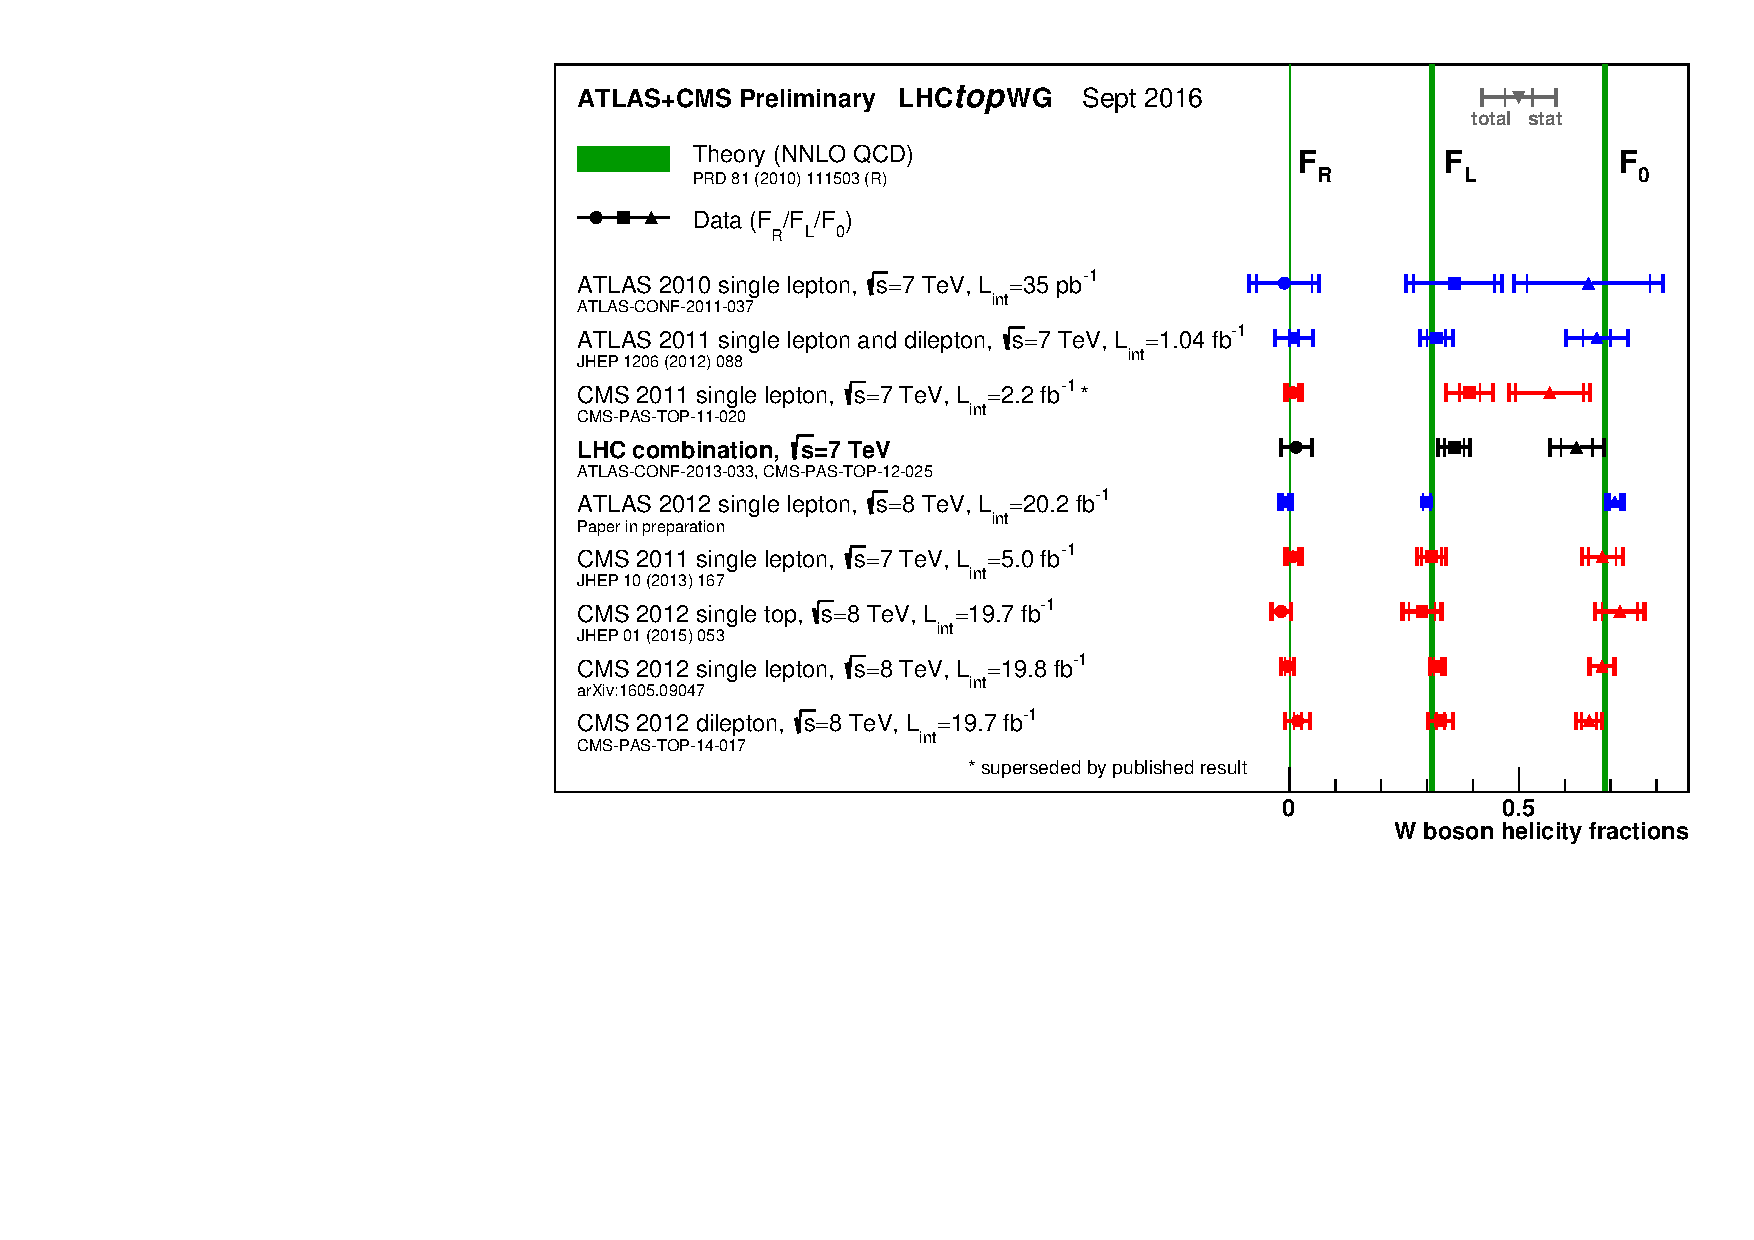
\includegraphics[width=0.95\textwidth]{figures/theory/LHC_W_helicity.pdf}
}

Overall, the various measurements presented here show a good agreement with the \gls{sm} prediction. Since no deviation is observed, limits on the anomalous couplings can be derived. Global fits of the anomalous couplings are however a complicated and computing-intense undertaking. Given a certain point in the coupling hyperspace, multiple observables need to be computed and compared to the results from various measurements while accounting for statistical and systematic uncertainties. A sophisticated fitting framework called \TOPFITTER[] has been recently developed~\cite{Buckley:2015lku}. The current estimated couplings strength per operator contributing to single-top-quark production obtained from various measurements at the \gls{lhc} and the Tevatron are shown in Fig.~\ref{fig:theory-eft-fit}. The results are found to be consistent with the \gls{sm} expectation where those operators vanish.

\myfigure[htbp]{\label{fig:theory-eft-fit}Coupling strength per operator contributing to single-top-quark production. Shown are 95\% confidence intervals. The Wilson coefficient $C_\mathrm{t}$ contains all contributions from four-fermion interactions. The figure is taken from Ref.~\cite{Buckley:2015lku}.}{
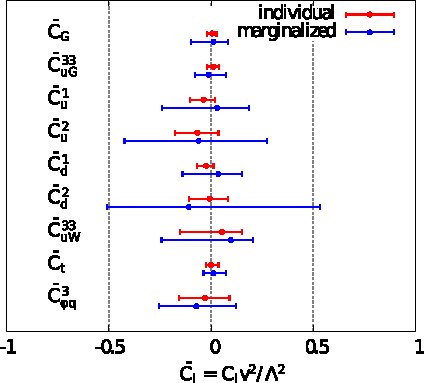
\includegraphics[scale=0.85]{figures/theory/EFT_fit.pdf}
}





%\chapter{Experimental setup}

\intro{The \glsreset{lhc}\gls{lhc}, its preacceleator chain and experiments are described. An emphasis is given on the CMS experiment. The data recorded with it in 2012, 2015, and 2016 at 8 and 13~\TeV are used in this thesis.}

\section{Large Hadron Collider}

\subsection{Accelerator complex}

\subsection{Experiments}

\section{CMS experiment}

\subsection{Magnet}

\subsection{Tracker}

\cite{Chatrchyan:2014fea}

\subsection{Electromagnetic calorimeter}

\subsection{Hadronic calorimeter}

\subsection{Muon systems}
DT/RPC/CSC

\subsection{Data acquisition}
Trigger/DAQ

\subsection{Operations}
DCS/DSS

%\chapter{Event reconstruction}
\label{ch:reconstruction}

\intro{The reconstruction of basic analysis objects within an event is described in this chapter. A key ingredient in the event reconstruction of \gls{cms} is the \acrfull{pf} algorithm. It creates particle candidates by combining various subdetector information for a global event interpretation which improves the identification, spatial resolution, and energy measurement of particles. The focus of this chapter is set on the reconstruction and performance of muons, electrons, jets, and the missing transverse energy in 8 and 13~TeV \gls{pp} collision data which are used to study single-top-quark production in this thesis. The chapter is concluded with a summary of corrections to enhance the agreement between data and simulation.}

The event reconstruction attempts to build and identify basic analysis objects from the raw detector data. In \gls{cms}, basic objects are charged-particle tracks, vertices, charged leptons, photons, and jet candidates. During the reconstruction, additional information such as the missing transverse energy, $\met$, and the likelihood of jets to originate from the hadronization of b~quarks~(``b-tagging'') is determined. Since tau leptons have not been utilized and photons are not relevant in the presented studies of $t$-channel single-top-quark production, a description of their reconstruction and performance is omitted here yet details can be found in Refs.~\cite{Khachatryan:2015dfa,Khachatryan:2015iwa}.


%##############################################
\section{Track reconstruction}
%##############################################
\label{sec:reconstruction-track}

The reconstruction of tracks from the readout of the inner tracking system consists of a local and a global reconstruction step. In the local reconstruction, hits from charge distributions on the pixel and strip modules are formed. Then, in the global reconstruction, trajectory candidates are first seeded and then sequentially built from the inside out. Finally, a helix track is fitted through the associated hits per trajectory candidate to estimate the particle's momentum and charge through its curvature in the magnetic solenoid field. An overview of the local and global reconstruction is given in the following. Further information can be found in Ref.~\cite{Chatrchyan:2014fea}.

Different algorithms are used to determine the local positions of two-dimensional (one-dimensional) hits from the distributions of charge deposits on the pixel (strip) modules, respectively. The pixel hit positions are estimated first with a fast algorithm whose outcome is used in the trajectory seeding and building stage only. The algorithm projects the 2D charge distributions onto each axis and estimates the positions from the charges at the edges of each charge cluster while accounting for their Lorentz-drift within the modules. During the track-fit stage, the optimal pixel hit positions are estimated by comparing the charge distributions against the expectations from simulated templates for various track incident angles~\cite{Swartz:2007zz}. In the barrel layers, a pixel hit resolution of $9.4~\upmu\mathrm{m}$ in $\mathrm{r}\mbox{-}\phi$ and between $21\range45~\upmu\mathrm{m}$ along the z-axis depending on the incident angle is achieved~\cite{Chatrchyan:2014fea}. 

For reconstructing hits on the strip modules, charge clusters are formed if the channel readout of adjacent strips is sufficiently above their individual noise levels. The hit position is then calculated as a charge-weighted average over a cluster while correcting for the Lorentz drift and potential inefficiencies which occur at the edges of a module. The hit resolution depends on the size of a cluster and on the strip-to-strip distance of the modules~(Sec.~\ref{sec:experiment-tracker}). It ranges roughly between $10\range30~\upmu\mathrm{m}$ ($10\range50~\upmu\mathrm{m}$) for the \gls{tib} (\gls{tob}) modules, respectively~\cite{Chatrchyan:2014fea}.

After the formation of hits, the reconstruction of tracks is performed in multiple passes, called iterations, over the obtained pixel and strip hit collections to reduce the combinatorial complexity. Each iteration consists of the same algorithmic steps---seeding, trajectory finding, track fitting, and selection---but is configured differently. The first iterations attempt to reconstruct only simple tracks which originate close to the interaction region and have a sufficiently large transverse momentum. The hits belonging to successfully reconstructed tracks passing certain quality criteria are then masked in subsequent iterations to reduce the number of hit combinations in the seeding and trajectory finding stages. Later iterations focus on reconstructing displaced or low momentum tracks which may not originate from the interaction region using the remaining hits. Figure~\ref{fig:reconstruction-trackingiter} shows the efficiency times acceptance for successfully reconstructing a track\footnote{Tracks are reconstructed ``successfully'' if at least 75\% of their hits can be associated to a simulated particle.} in simulation, broken down per iteration, as a function of its transverse momentum or displacement.

\myfigure{\label{fig:reconstruction-trackingiter}The efficiency times acceptance of successfully reconstructing a track in simulation per tracking iteration as a function of (a)~the transverse momentum and (b)~the transverse displacement. The figures are taken from Ref.~\cite{trackingpublic}.}{
\subfloat[]{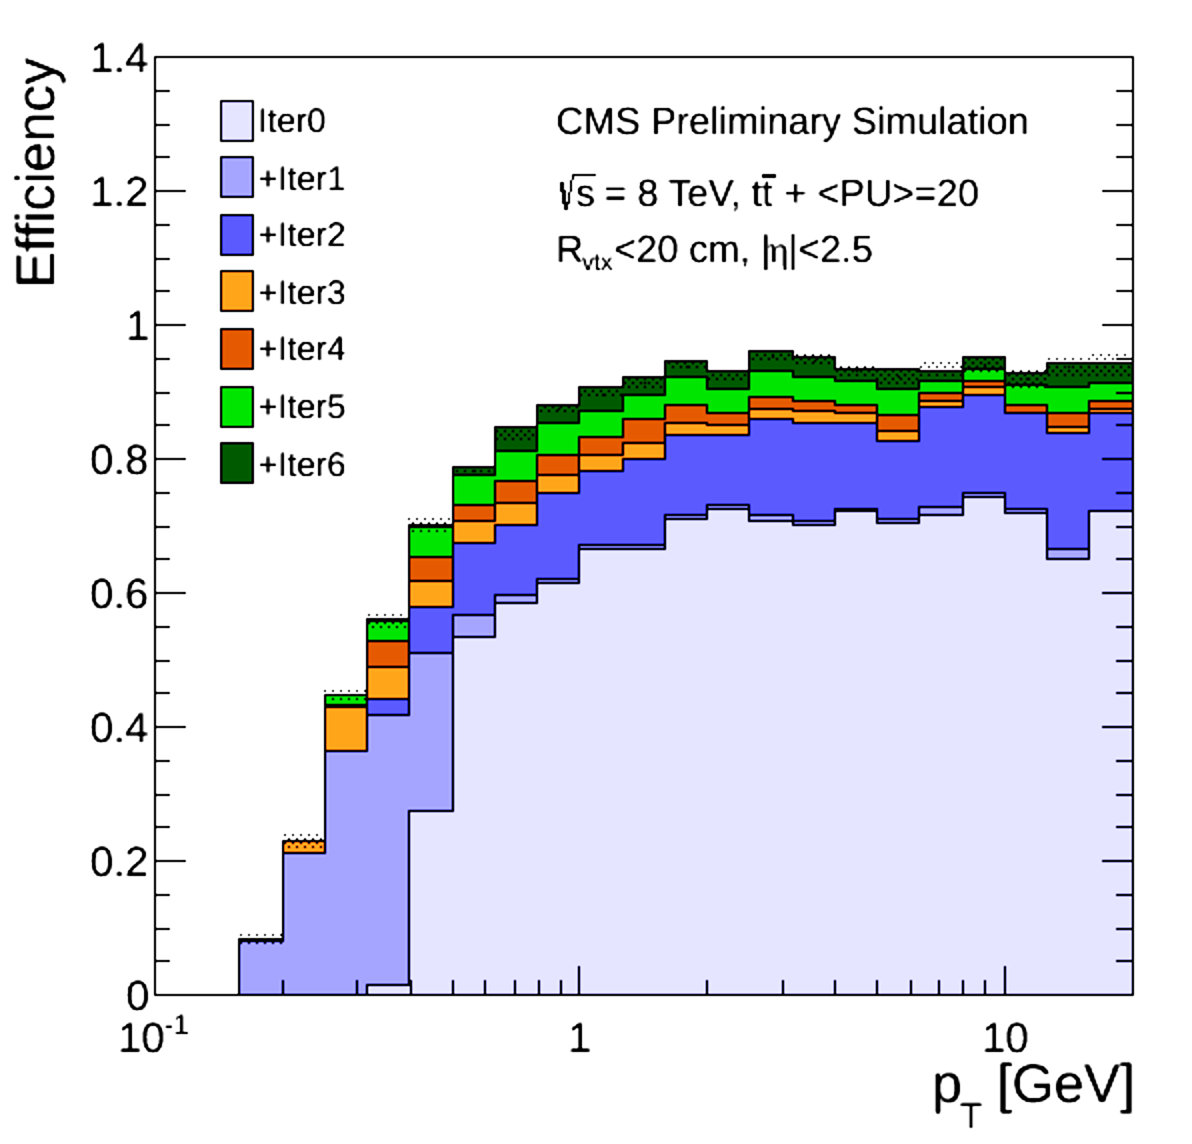
\includegraphics[width=0.48\textwidth]{figures/reconstruction/tracking_vs_pt.jpg}}\hspace{0.03\textwidth}
\subfloat[]{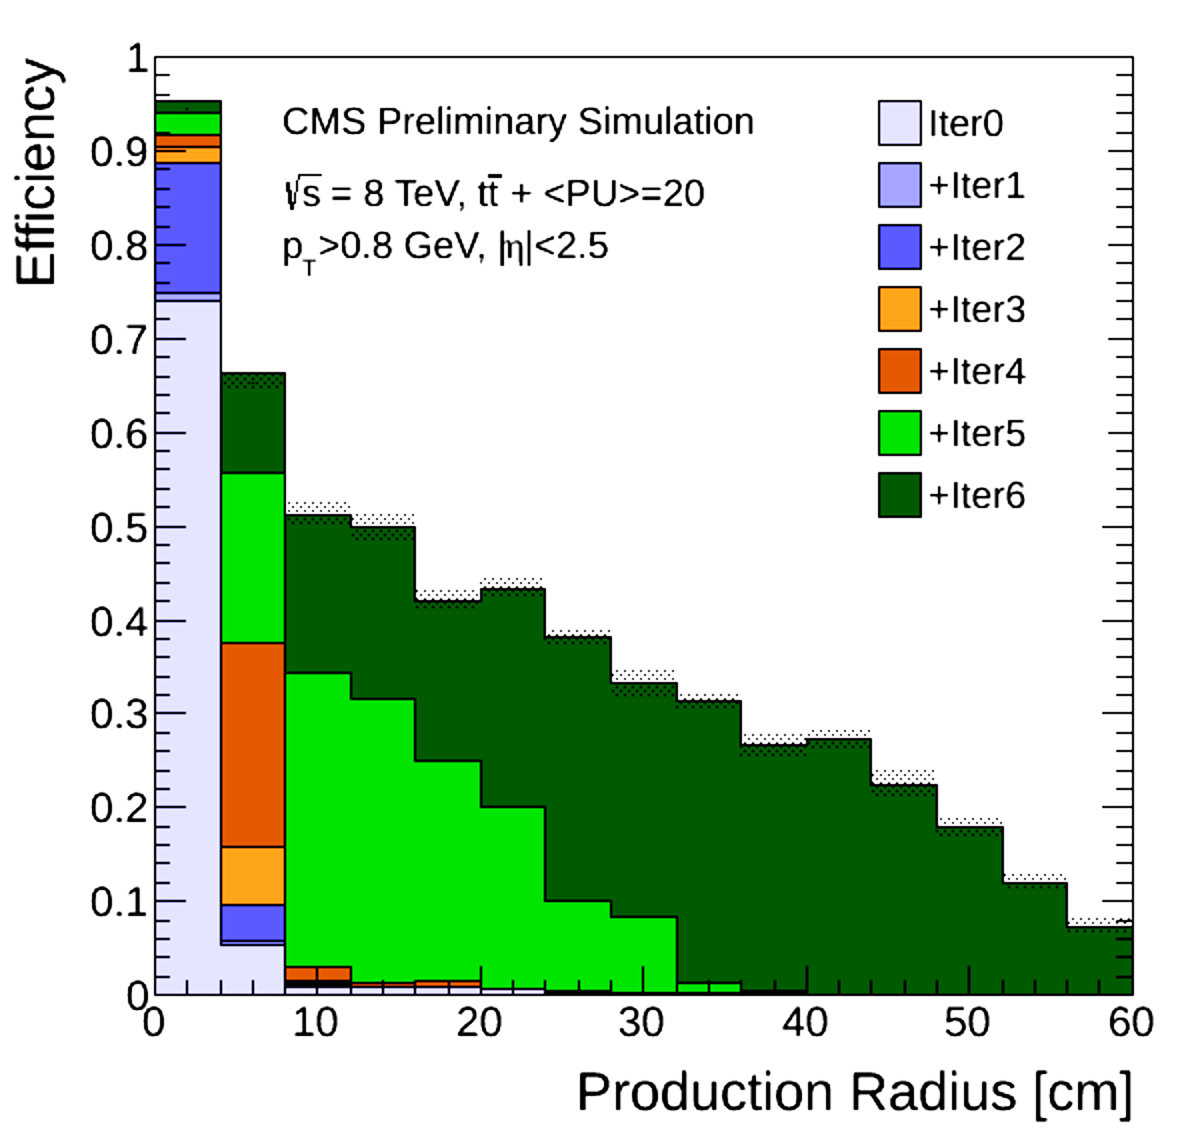
\includegraphics[width=0.48\textwidth]{figures/reconstruction/tracking_vs_vertpos.jpg}}
}

Each iteration commences by forming a trajectory seed from a hit doublet or triplet where only certain combinations of tracker layers are allowed depending on the iteration. First iterations utilize mostly 3D hits on the pixel layers for seeding since their low channel occupancy results in less ambiguity and a higher efficiency for close-by tracks. Late iterations use hits from the strips modules instead where the spatial track density is low. Here, 3D matched hits are utilized mostly for seeding which stem from double-sided strip modules but also hits from mono layers are allowed. Seed candidates have to fulfill certain quality criteria like a minimal transverse momentum and compatibility with either the beam spot or a preliminary reconstructed vertex depending on the iteration before they are passed to the trajectory finding stage.

Each seed contains enough information to perform a first estimate of the track parameters. Then an algorithm called \glshere{ctf} extrapolates the estimated trajectory to find additional hits on subsequent layers which are compatible with a particle track hypothesis. The \gls{ctf} algorithm is based on the \glshere{kf} technique~\cite{Fruhwirth:1987fm,Billoir:1989mh,BILLOIR1990219} which describes how to update the track parameters and their uncertainties iteratively after adding a hit to the trajectory candidate. If multiple compatible hits are found on a layer, the trajectory is cloned for each of them. If no compatible hit can be found on a layer a ghost hit is created instead.

The hits per trajectory are then passed to a \gls{kf}-based helix fit to estimate the track parameters without utilizing the initial estimate from the seed. In addition, the fit accounts for material effects and the inhomogeneous magnetic field.  The fitted tracks have to pass a quality selection to reduce the amount of fake tracks before they are considered in physics analyses. The criteria reflect the seed requirements and depend additionally on the total number of fitted 2D/3D hits, the $\chi^2/\mathrm{\gls{ndof}}$ of the fit, the amount of ghost hits, and the amount of shared hits with other tracks amongst others.

The tracking efficiency for isolated muon tracks with $1<\pt<100~\GeV$ is found to be above $99\%$ over the full tracker acceptance since their trajectories are only disturbed by energy loss through ionization and Coulomb scattering. The trajectories of charged hadrons like pions are additionally affected by nuclear interactions, especially at low momenta ($\pt<700~\MeV$), which results in efficiencies between $80\range95\%$~\cite{Chatrchyan:2014fea}. For electrons, a special tracking is performed on top of the standard one (described in Sec.~\ref{sec:reconstruction-electrontracks}) which attempts to recover cases where the electron looses large amounts of energy via bremsstrahlung. In parts of the 2016 collision data the overall tracking efficiency decreased by about $2\range6\%$ at high instantaneous luminosities of $10\range12~\mathrm{Hz/nb}$ due to a charge saturation effect on the readout chips leading to missing hits. This has been recovered by adjusting the voltage which controls the charge drain speed of the tracker modules. For already collected data, the effect has been mitigated offline while any residual loss of efficiency is known and accounted for through dedicated scale factors.

%##############################################
\subsection{Muon tracks}
%##############################################
\label{sec:reconstruction-muontracks}

The track reconstruction for muons begins with the local reconstruction of hits in the three muon systems~\cite{Bayatian:922757}. The positions of hits in the \gls{dt} system are reconstructed by first forming independent segments in $r\text{-}\phi$ and $r\text{-}z$ through a combination of pattern recognition and linear fitting steps which are then combined in a second step. For the \glspl{csc}, independent 2D hits are reconstructed at wire--strip intersections in each of the six layers which are then combined into a track segment through a linear fit. Hits in the \gls{rpc} modules are built from clusters of active strips where their positions are taken as the center of gravity of the cluster's area.

Standalone muon tracks are reconstructed from hits in the muon system only without using the inner tracker. The muon tracking starts by generating seeds from linear fits through hits in the \gls{dt} and \gls{csc} systems. Then, \gls{kf}-based track fits are performed taking as starting point the seeds while also utilizing the hits in the \gls{rpc} system. In addition, the resulting track is constrained to be close to the beam spot which improves the momentum resolution. A global muon track is reconstructed by extrapolating the standalone muon track inwards to define a region of interest inside the inner tracking system. Starting from trajectory seeds inside this region, a global muon trajectory is built and fitted which employs also compatible hits from the inner tracker.


%##############################################
\subsection{Electron tracks}
%##############################################
\label{sec:reconstruction-electrontracks}

In \gls{cms}, an electron radiates more than 70\% of its energy with a probability of 35\% in the inner tracker through bremsstrahlung before reaching the \gls{ecal}. This leads to an increasingly curved electron trajectory in the magnetic field as a function of its flight distance. The standard tracking is suboptimal for reconstructing such trajectories because the employed Kalman filtering assumes that the energy loss is Gaussian-distributed. Therefore, a different filtering algorithm the so-called \glshere{gsf}~\cite{0954-3899-31-9-N01} is used in the electron tracking reconstruction instead.

Trajectory seeds for the \gls{gsf} tracking are constructed in two ways. The first method creates \gls{ecal}-driven seeds by forming super clusters of \gls{ecal} crystals with a size of 0.09 in $\eta$ but $\pm0.3~\mathrm{rad}$ azimuthally to capture electrons together with their potentially radiated photons~\cite{CMS:2010aua}. The second method tries to identify electron tracks inside the standard track collection which are typically marked by either a poor fit quality if the energy loss was large or by its compatibility with an \gls{ecal} cluster otherwise. The resulting seeds from the two methods are selected to initiate the \gls{gsf} tracking. In its core, the algorithm book-keeps a set of trajectories which are subjected to the standard \gls{kf}-based tracking algorithm. However, different Gaussian distributions are assumed for the energy loss per trajectory while their sum is an approximation of the Bethe-Heitler formula per hit describing the probability of energy loss for electrons via bremsstrahlung. After extrapolating a trajectory set to a new layer, incompatible trajectories are removed or merged with similar ones to limit the exponential growth to a maximum of 12 trajectories per set. The final electron track is estimated by using the summed Gaussian distributions as uncertainties per hit in the track fit. 

The electron reconstruction efficiency has been measured in 8~TeV \gls{pp} collision data to be better than 93\% for electrons with an \gls{ecal} super cluster energy of $E_\mathrm{T}>20~\GeV$~\cite{Khachatryan:2015hwa}. A tracking efficiency of about 96\% is obtained for electrons with $E_\mathrm{T}>25~\GeV$ in 13~\TeV \gls{pp} collision data~\cite{CMS-DP-2017-004}.



%##############################################
\section{Vertex reconstruction}
%##############################################


The vertex reconstruction tries to locate points of \gls{pp} interactions which are identified by sets of close-by charged-particle tracks in the interaction region. In analyses, the association of tracks to vertices allows to separate tracks belonging to the hard scattering from additional tracks which originate from pileup interactions instead.

The first step in the vertex reconstruction encompasses the forming clusters of spatially-close tracks. For this, tracks which are close to the beam spot are selected and supplied to a \glshere{da} algorithm~\cite{726788}. It is based on a statistical mechanics model where each track reflects a microstate. The association of a track to a vertex candidate is floating and controlled by a probability denoted $p_{i}$ in the following. A quantity

\begin{equation}
F=-T\sum_{i}^\mathrm{tracks}\,p_{i}\cdot\Bigg(\sum_{j}^\mathrm{vertices}\,\rho_{j}\cdot\exp\Big[-\big(z_{i}^\scriptn{\mathrm{(track)}}-z_{j}^\scriptn{\mathrm{(vertex)}}\big)^2\Big/\big(T\cdot\sigma_{z,i}^2\big)\Big]\Bigg)\,,
\end{equation}
 
which is an analog of the free energy in a thermodynamical model, is monitored while decreasing the corresponding temperature $T$ of the system. Here, $z_{i}$ are the track/vertex positions, $\sigma_{i}$ denotes the uncertainty of the track positions, and $\rho_{k}$ is an additional weight to treat overlapping vertices effectively. A protovertex is split in two nearby ones if a minimum of the free energy is reached. The decrease of temperature is stopped when a trade-off between the expected spatial vertex resolution and the probability of splitting a proper vertex falsely is reached.

Finally, the optimal vertex positions are estimated through an adaptive vertex fit~\cite{0954-3899-34-12-N01} per cluster of tracks. The obtained vertices are referred to as ``primary vertices'' since they mark the point of a \gls{pp} interaction and are therefore lined up along the z-axis. The vertices are ordered by the summed $\pt^2$ of their associated tracks where the leading vertex is assigned to mark the hard interaction of interest while the others are treated as pileup interactions. In 2016 \gls{pp} collision data, the primary vertex resolution is measured as $\sigma_{z}\leq19~\upmu\mathrm{m}$ and $\sigma_{x,y}\leq14~\upmu\mathrm{m}$ for vertices whose summed \pt of associated tracks exceeds $100~\GeV$~\cite{CMS-DP-2016-041}.



%##############################################
\section{Particle flow}
%##############################################

A central element in the standard event reconstruction of \gls{cms} is the \glshere{pf} algorithm~\cite{Sirunyan:2017ulk,CMS:2009nxa}. It aims at reconstructing global particle candidates like electrons, muons, photons, and charged and neutral hadrons in an event by tracing the flow of particles through the various subdetectors. The combination of the individual subdetector information leads to an improved spatial resolution, energy measurement, and type identification of particles while avoiding double counting.

The \gls{pf}-based reconstruction of particles consists of an algorithm to link information from several subdetectors together. The linked elements can be charged-particle tracks from the inner tracking system, calorimeter clusters from the \gls{ecal} or \gls{hcal}, and muon tracks. The algorithm starts by extrapolating reconstructed charged-particle tracks from the inner tracking system into the calorimeter systems. In the \gls{ecal}, the trajectories are extended to the expected depth of the shower maximum of an electron candidate whereas in the \gls{hcal}, the trajectories are extrapolated up to one interaction length. A link is created if a trajectory is located inside the boundaries of a compatible \gls{ecal} or \gls{hcal} cell cluster within uncertainties. Photon candidates, which could have been emitted tangentially from electron tracks, are also created by extrapolating straight tracks from intersections of the electron track with the tracker layers to compatible \gls{ecal} cells. For neutral particle candidates links between calorimeter clusters are formed. Here, the algorithm starts with \gls{ecal} clusters for which a good resolution is expected due to their high granularity and extrapolates them to potential \gls{hcal} clusters which has a coarser granularity. Links are also created from the \gls{es} to clusters in the coarser \gls{ecal} endcaps. A link between a tracker track and the muon system is created if the described track reconstruction of a global muon~(Sec.~\ref{sec:reconstruction-muontracks}) yields an acceptable goodness-of-fit.

Identification of particles is performed by exploiting the different types of information from the linked blocks. First, global \gls{pf} muons are identified if their momenta are compatible with the corresponding tracker-only track momenta. Next, \gls{pf} electrons are identified through the \gls{gsf} tracking together with potential photons from bremsstrahlung. A \gls{pf} charged hadron candidate is created for each of the remaining \gls{pf} candidates that have a charged-particle track linked to it. Finally, the amount of neutral energy is determined by subtracting the charged particle energy fraction from the calibrated energy of the linked calorimeter clusters. This procedure yields \gls{pf} photon and \gls{pf} neutral hadron candidates depending on the excess of neutral energy in the \gls{ecal} and \gls{hcal} clusters respectively. Outside the acceptance of the inner tracking system ($|\eta|>2.4$), no information on the particle's charge is available. Thus, only a simplified identification is performed by constructing either hadronic or electromagnetic \gls{pf} candidates only. In a pseudorapidity range of $2.4<|\eta|<3$, such candidates are formed from \gls{ecal}/\gls{hcal} clusters, whereas in $3<|\eta|<5$ the difference between the readouts of the long and short fibers of the \gls{hf} calorimeter allows to discriminate between these two types.

The achieved improvement in spatial and energy resolution through the \gls{pf} algorithm is demonstrated exemplary for jets in Fig.~\ref{fig:reconstruction-pfjets}. In particular, the energy resolution at low momenta is significantly improved compared to jets clustered from calorimeter cells only since the jet energy estimation in the \gls{pf} algorithm exploits also the measured momenta of charged-particle tracks from the inner tracking system.

\myfigure{\label{fig:reconstruction-pfjets}Comparison of simulated calorimeter and particle flow jet performances: (a)~spatial resolution in $\eta$; (b)~energy resolution. The figures are taken from Ref.~\cite{CMS:2009nxa}.}{
\subfloat[]{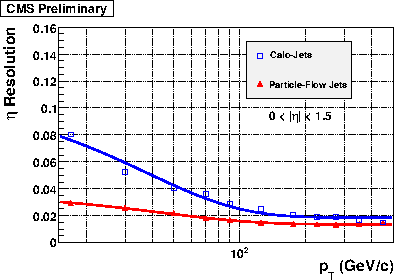
\includegraphics[width=0.48\textwidth]{figures/reconstruction/pf_jeteta.pdf}}\hspace{0.03\textwidth}
\subfloat[]{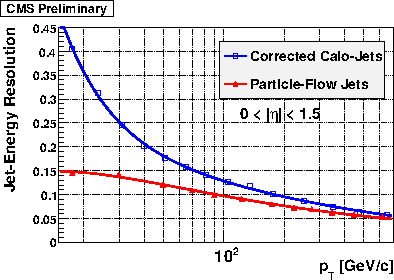
\includegraphics[width=0.48\textwidth]{figures/reconstruction/pf_jetenergy.pdf}}
}

%##############################################
\section{Muons}
%##############################################
\label{sec:reconstruction-muons}

Identification of muon candidates for physics analyses is performed by requiring additional selection criteria. A detailed study of muon identification with 7~\TeV \gls{pp} collision data can be found in Ref.~\cite{Chatrchyan:2012xi}. Throughout the analyses within this thesis, muon candidates have to fulfill identification criteria which correspond to a ``tight'' working point yielding most genuine muons while rejecting falsely reconstructed ones. In the following, the criteria and performance of muon identification employed in the analysis of 8~TeV and 13~\TeV \gls{pp} collision data within this thesis are briefly discussed. Detailed reports on their performance can be found in Ref.~\cite{CMS-DP-2013-009,CMS-DP-2017-007}.

The muon identification criteria are as follows. The global muon fit is required to included at least one valid hit in the muon chambers for which in addition at least two muon segments in two muon stations are present. Only muon tracks for which the global track fit yields a goodness-of-fit of $\chi^\scriptn{2}/\mathrm{\gls{ndof}}<10$ are selected. The motivation behind these criteria is to reject fake muons from hadron showers that are not contained by the \gls{hcal} and reach the muon system~(so-called ``punch-throughs''). To suppress the decay of muons in flight, the muon track needs to consist of at least one pixel hit. Additionally, a minimum number of five hits in the tracker is required. A selection on the minimal distance of the muon track to the primary vertex of $d_{x,y}<2~\mathrm{mm}$ and $d_{z}<5~\mathrm{mm}$ is applied to reject cosmic muons and muons stemming from \gls{pu} interactions. A comparison of muon identification efficiencies for data and simulation is presented in Fig.~\ref{fig:reconstruction-idmuon}. These have been estimated using the tag-and-probe method for which $\mathrm{Z}\to\mu^{\rmplus}\mu^{\rmminus}$ events are selected where one muon is required to pass the identification criteria~(``tag''). It is then measured in how many instances the other muon fulfills the identification criteria as well~(``probe'') to infer the efficiency. The efficiency is found to be mostly between 95\range100\% with the exception of two dips at $0.2<|\eta|<0.3$ which occur due to a crack between the wheels of the \gls{dt} system. Overall, a fair agreement between data and simulation is observed. The residual differences are corrected in simulation by applying $(\pt,\eta)$-dependent scale factors ($\epsilon_\mathrm{data}/\epsilon_\mathrm{MC}$) to simulated events.

\myfigure{\label{fig:reconstruction-idmuon}Comparison of muon identification efficiencies in data and simulation as a function of the pseudorapidity of the muon for analyses at (a)~8~TeV and (b)~13~\TeV. The figures are taken from Refs.~\cite{CMS-DP-2013-009,CMS-DP-2017-007}.}{
\subfloat[]{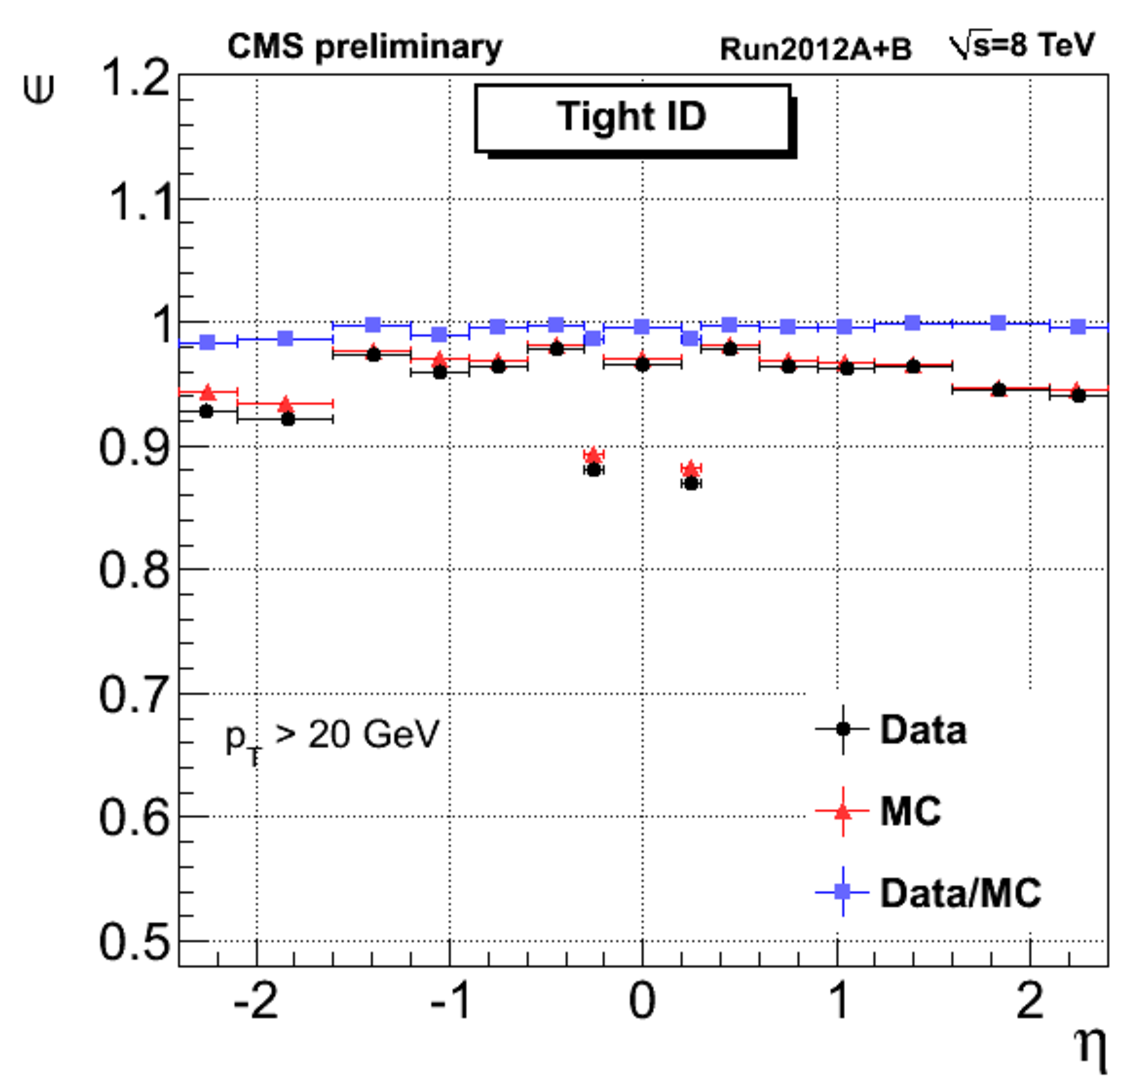
\includegraphics[width=0.48\textwidth]{figures/reconstruction/muon_id8.pdf}}\hspace{0.03\textwidth}
\subfloat[]{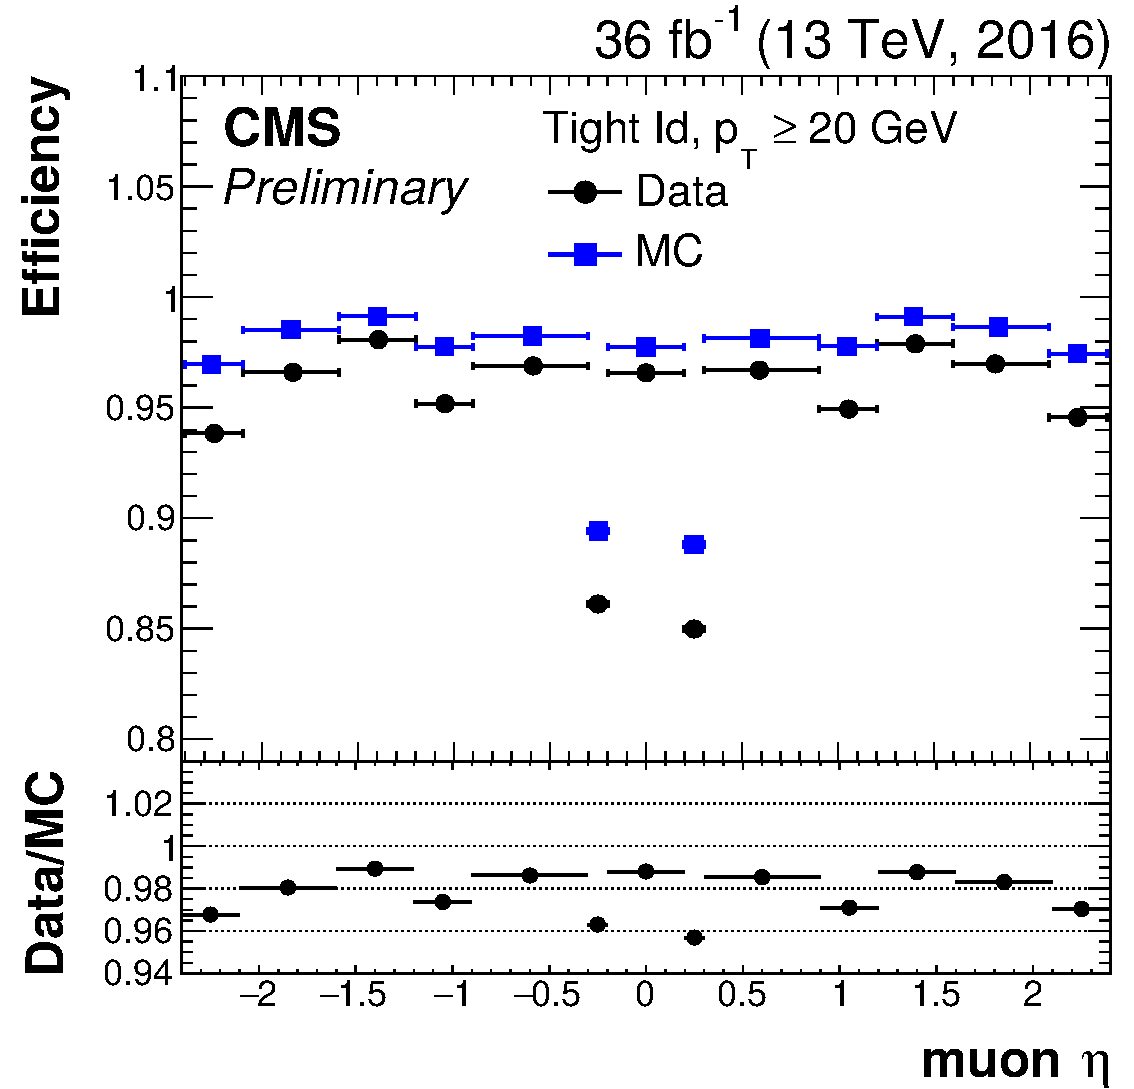
\includegraphics[width=0.48\textwidth]{figures/reconstruction/muon_id13.pdf}}
}

Muon candidates in the analyses of single-top-quark production within this thesis are required to be spatially isolated from \gls{em} and hadronic activity in addition to the tight identification criteria. The relative \gls[format=hyperbf]{deltabeta}-based (``delta-beta'') isolation for muons is defined as

\begin{equation}
I_\mathrm{rel.}^{\mu}=\frac{I_\text{ch.-had.}+\max\Big(0,~I_{\gamma}+I_\text{neut.-had.}-\beta\cdot I_\text{\gls{pu}}\Big)}{\pt^\mu}\,,\qquad \beta=\frac{1}{2}\,,
\end{equation}

where $I_\text{ch.-had.}$, $I_{\gamma}$, and $I_\text{neut.-had.}$ denote the summed transverse energies of charged hadrons, photons, and neutral hadrons respectively within $\Delta R=\sqrt{\Delta\eta^{2}+\Delta\phi^{2}}<0.4$ around a muon candidate. The term $I_\text{\gls{pu}}$ is used to correct the amount of considered neutral energy. It denotes the summed transverse energies of charged-particle tracks within $\Delta R<0.4$ that are associated to pileup vertices. Hence, the applied correction $\beta\cdot I_\text{\gls{pu}}$ can be interpreted as an estimate of the amount of neutral energy from pileup interactions within $I_{\gamma}$ and $I_\text{neut.-had.}$. The chosen value for $\beta$ is motivated by assuming equal production rates for the ($\uppi^{\rmplus}$,$\uppi^{0}$,$\uppi^{\rmminus}$) isospin triplet leading to a ratio of $\sfrac{1}{2}$ for the production of neutral pions over charged ones. 


%##############################################
\section{Electrons}
%##############################################
\label{sec:reconstruction-electrons}

Similar to muon candidates, electron candidates are required to pass certain identification criteria as well. Studies of the electron reconstruction and identification performances in 8~\TeV and 13~\TeV \gls{pp} collision data can be found in Refs.~\cite{Khachatryan:2015hwa,CMS-DP-2017-004}. The ``tight'' identification criteria, employed in this thesis, are elaborated briefly in the following.

A \gls{pf} electron candidate with a \gls{gsf} track is required. Candidates within the \gls{ecal} barrel-endcap transition region of $1.4442<|\eta|<1.5660$ are ignored. The electron track has to have a hit on the innermost tracker layer which prevents the selection of electrons from potential photon conversions~($\gamma\to\mathrm{e}^{\rmplus}\mathrm{e}^{\rmminus}$). An explicit photon conversion veto is applied by testing if a pair of electron tracks originates from a common displaced vertex. Further selection criteria are combined into a multivariate identification discriminant. It is based on various input observables like the \gls{gsf} track quality, the \gls{ecal} cluster shapes, their energy distribution, and the agreement between the independent cluster energy and track energy estimates. For 13~TeV data, the discriminant is replaced by a simplified cut-based version where multiple fined-tuned selections on similar observables are applied. A comparison of the efficiency of electron identification in 8~TeV data and simulation, estimated from $\mathrm{Z}\to\mathrm{e}^{\rmplus}\mathrm{e}^{\rmminus}$ events using the tag-and-probe method, is shown in Fig.~\ref{fig:reconstruction-idelectron}. For transverse momenta above $30~\GeV$ the identification reaches efficiencies of $\approx95\%$. The small differences between data and simulation are corrected by dedicated scale factors as well, similar to the treatment of muon identification efficiencies~(Sec.~\ref{sec:reconstruction-muons}).

\myfigure{\label{fig:reconstruction-idelectron}Comparison of the electron identification efficiency in data and simulation as a function of its transverse momentum. The figure is taken from Ref.~\cite{CMS-DP-2013-003}.}{
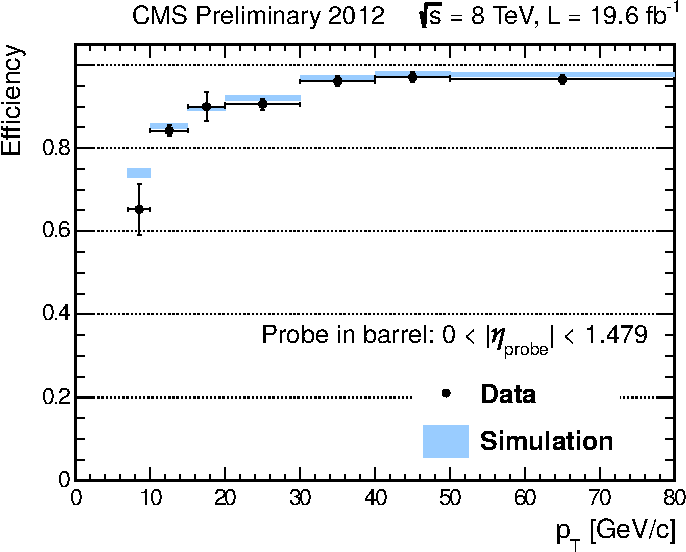
\includegraphics[width=0.55\textwidth]{figures/reconstruction/electron_idpt1_1.pdf}
}

An electron candidate is also required to be isolated from other \gls{em} or hadronic activity in its vicinity. The relative \gls[format=hyperbf]{effarea}-based (``effective area'') isolation for electrons is defined as

\begin{equation}
I_\mathrm{rel.}^\mathrm{e}=\frac{I_\text{ch.-had.}+\max\Big(0,~I_{\gamma}+I_\text{neut.-had.}-\rho\cdot A_\text{eff.}(\eta_\mathrm{SC})\Big)}{\pt^\mathrm{e}}\,,
\end{equation}

where the transverse energies $I_{X}$ per particle type $X$ are summed in a cone of $\Delta R<0.3$ around the electron candidate. The amount of neutral energy is corrected by the effective area $A_\text{eff.}$ times the median of the transverse energy density $\rho$ calculated in $\delta\eta\times\delta\phi$ from charged-particle tracks that are associated to pileup vertices. The effective area is estimated from simulation and denotes the expected amount of neutral energy from pileup interactions per $\rho$ within the isolation cone as a function of the pseudorapidity of the associated \gls{ecal} supercluster. The general idea behind the \gls{effarea}-based isolation for electrons is motivated by a proposed pileup subtraction method for jets which is detailed in Ref.~\cite{Cacciari:2007fd}.


%##############################################
\section{Jets}
%##############################################
\label{sec:reconstruction-jets}

Jets are clustered from \gls{pf} candidates with the exclusion of charged hadrons that are associated to pileup vertices. This procedure is referred to as \glshere{chs} technique~\cite{CMS-PAS-JME-14-001}. In addition, preselected isolated muons or electrons can be excluded from the jet clustering as well to prevent double counting of their momenta. For example, when studying the decay $\mathrm{t}\to \mathrm{b}\mu\nu$ a selected muon candidate should be prevented from being clustered into the b~jet as well. This approach has been chosen in the reconstruction of 8~TeV data, whereas in analyses of 13~TeV data a minimal $\Delta R$ distance between the final leptons and jets for analysis is required instead.

Jets are clustered using the iterative anti-\kt algorithm~\cite{Cacciari:2008gp}. In its initial step all candidates are considered to be so-called ``protojets''. At each iteration step the two distances

\begin{equation}
d_{ij}=\mathrm{min}\left(\frac{1}{p_{\mathrm{T},i}^{2}},\,\frac{1}{p_{\mathrm{T},j}^{2}}\right)\cdot\frac{\sqrt{\Delta\eta_{ij}^{2}+\Delta\phi_{ij}^{2}}}{\mathrm{R}^2}\,,\qquad d_{i}=\frac{1}{p_{\mathrm{T},i}^{2}}\,,
\end{equation}

are calculated for protojets $i$ and $j$.  If $d_{ij}$ is the smallest distance between two protojets in an iteration, they are merged and their 4-momenta are summed. If otherwise $d_{i}$ is found to be the smallest distance, the corresponding protojet is promoted to a final jet and ignored in subsequent steps. The parameter $\mathrm{R}$ controls the cone size of the resulting jets. In 8~TeV data, jets are clustered with $\mathrm{R}=0.5$ which was lowered to $\mathrm{R}=0.4$ in the reconstruction of 13~TeV data since the objects are more boosted due to the higher energy resulting into a smaller cone size.

In this thesis a ``loose'' jet identification is applied. The criteria are motivated by the fact that a proper jet, stemming from the hadronization of a quark or gluon, consists of a multitude of \gls{pf} particles and types. The exact criteria are somewhat adjusted from one data taking period to the next. A few common requirements are detailed in the following. A jet should consists of more than one constituent and the neutral hadron and neutral \gls{em} energy fractions should be both less than $99\%$. In addition, for jets that fall within the tracker acceptance~($|\eta|<2.4$) at least one constituent has to be a charged hadron and the charged \gls{em} fraction is required to be less than $99\%$ amongst others. The identification efficiencies are found to be very close to 100\% for both data and simulation.

In data and simulation the energies of reconstructed jets are found to deviate from the energies of corresponding jets clustered from the hadronization products of true partons from simulation due to non-linear subdetector responses and efficiencies. Therefore a series of \glsplhere{jec} are applied to relate the reconstructed energy to the true jet energy on average. The applied corrections are briefly outlined in the following whereas a detailed discussion can be found in Ref.~\cite{Khachatryan:2016kdb}. The \glspl{jec} are multiplicative factors for rescaling the 4-momenta of jets. Multiple levels of corrections are applied to data and simulation sequentially. First, the offset correction removes the dependence of the jet energy response on the additional pileup activity within an event. It is based on the jet area method~\cite{Cacciari:2007fd}. The correction factors are derived by comparing the jet responses in simulated events with and without pileup events overlaid. The next level of corrections aims to obtain a uniform energy response which is independent of the transverse momentum and pseudorapidity of a jet. The corrections are derived from simulated events by matching reconstructed jets to close-by true particle jets and comparing their momenta. Lastly, residual differences between data and simulation are corrected by comparing the $\pt$ balance in various  types of events~(multijet, \mbox{$\mathrm{Z}$+jets}, \mbox{$\gamma$+jets}) where one jet is restricted to be within the barrel region~($|\eta|<1.3$) to provide a reference. The total and individual uncertainties from the various corrections are shown in Fig.~\ref{fig:reconstruction-jec} for 8~\TeV and 13~\TeV data. At 8~\TeV, the uncertainty is found to be mostly around $1\%$ and only approaches $2\%$ for forwards jets~($|\eta|>3$) with low transverse momenta of $\pt\approx30~\GeV$, whereas larger uncertainties of 3\range5\% are found at 13~\TeV for jets with a transverse momentum of $30~\GeV$ and above. The optional jet flavor corrections shown in the plots have not been applied in the measurements within this thesis.

\myfigure[h!tb]{\label{fig:reconstruction-jec}Uncertainty on the \acrlongpl{jec} as a function of (left column)~the transverse momentum and (right column)~the pseudorapidity for \acrlongpl{cm} energies of (top row)~8~\TeV and (bottom row)~13~\TeV. The figures are taken from Refs.~\cite{Khachatryan:2016kdb,CMS-DP-2016-020}.}{
\subfloat[]{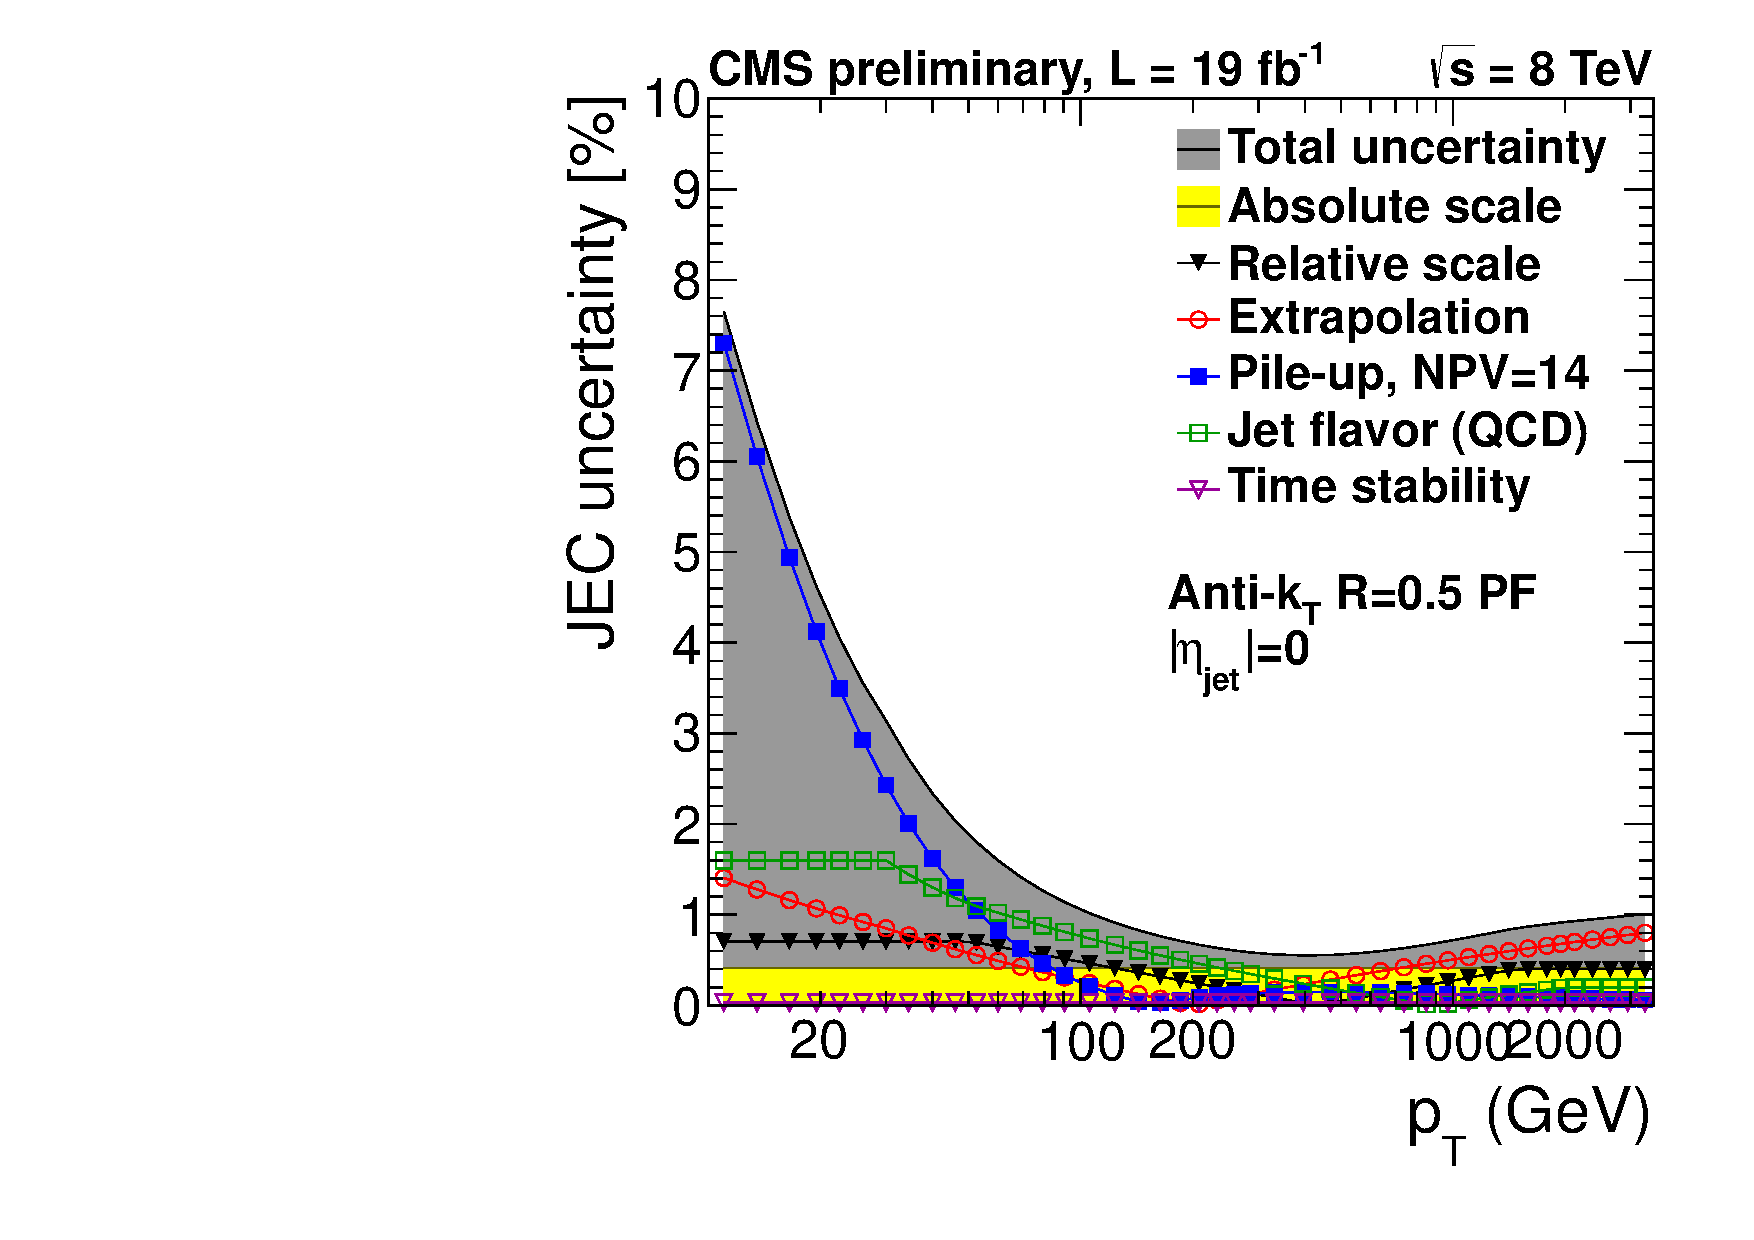
\includegraphics[width=0.48\textwidth]{figures/reconstruction/jet_uncpt.pdf}}\hspace{0.03\textwidth}
\subfloat[]{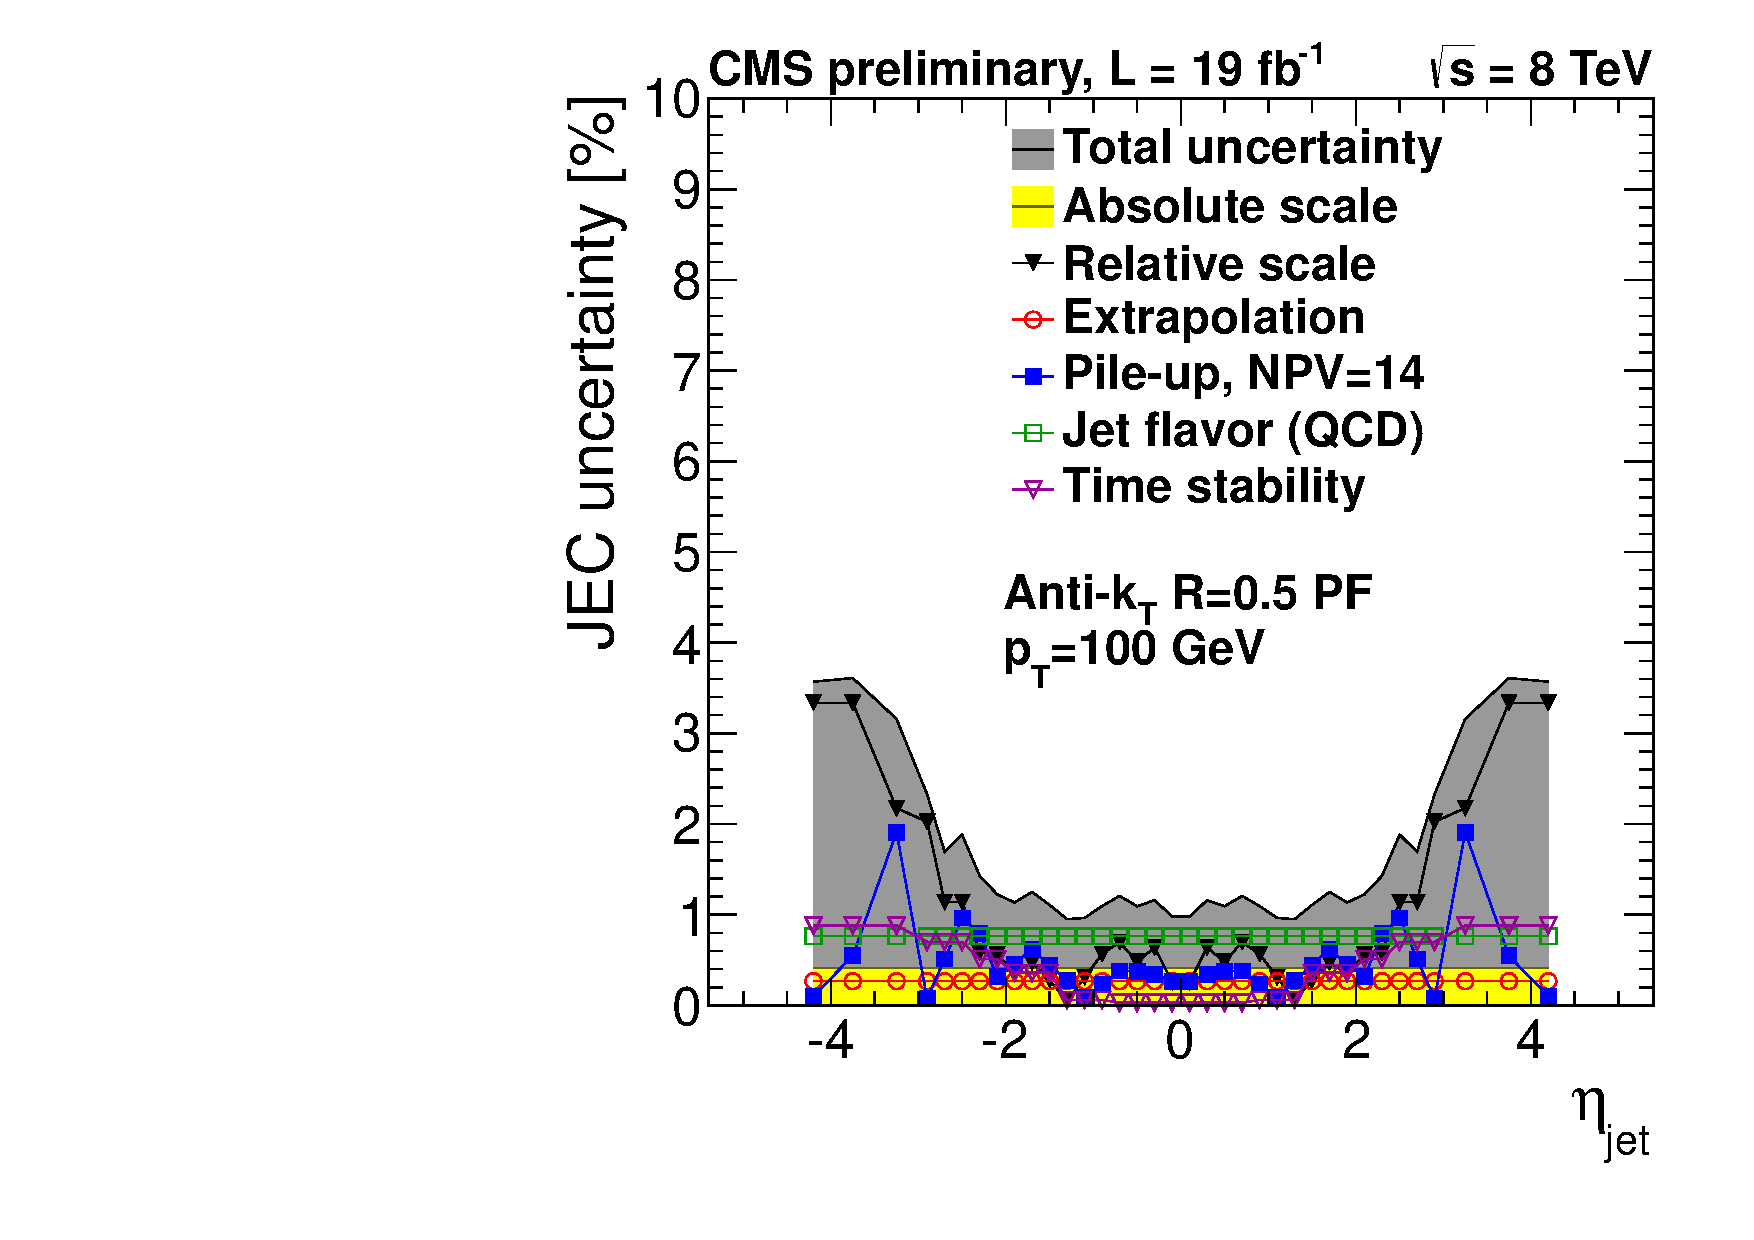
\includegraphics[width=0.48\textwidth]{figures/reconstruction/jet_unceta.pdf}}\\
\subfloat[]{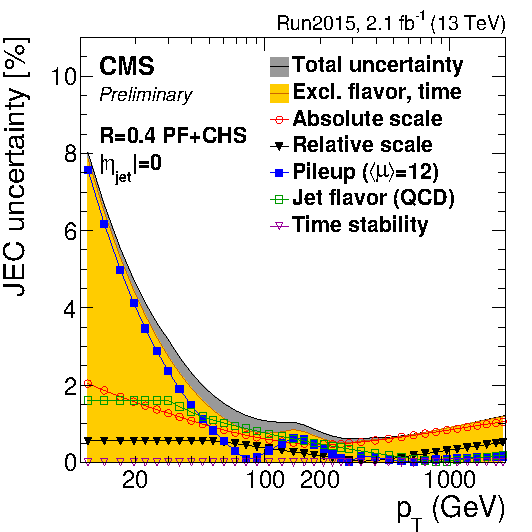
\includegraphics[width=0.48\textwidth]{figures/reconstruction/jet_uncpt13.pdf}}\hspace{0.03\textwidth}
\subfloat[]{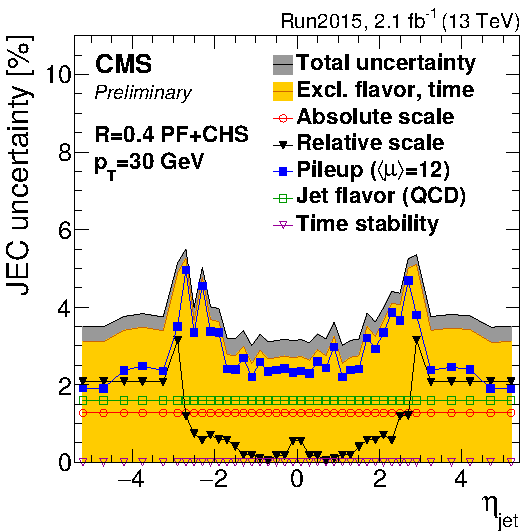
\includegraphics[width=0.48\textwidth]{figures/reconstruction/jet_unceta13.pdf}}
}

In addition to rescaling the jet energy, the \glshere{jer} is corrected for simulated jets to mimic the spread in $\pt$ as observed in data. Exemplary relative resolutions in terms of $\pt^\mathrm{reco.}/\pt^\mathrm{true}$ in 8~TeV simulation are presented in Fig.~\ref{fig:reconstruction-jer-spread} for various pileup scenarios. Two methods are used to rescale the reconstructed 4-momentum which are chosen whether or not a jet can be matched to a true jet in simulation. The factors are defined as

\begin{subequations}
\begin{align}
c_\mathrm{matched}&=1+\frac{\pt^\mathrm{reco.}-\pt^\mathrm{true}}{\pt^\mathrm{reco.}}\cdot\big(s_\mathrm{\gls{jer}}-1\big)\,,\label{eq:reconstruction-jer-matched}\\ c_\mathrm{unmatched}&=1+\mathsf{N}(0,\,\sigma_\mathrm{\gls{jer}})\cdot\sqrt{\mathrm{max}\big(s_\mathrm{\gls{jer}}^2-1,\,0\big)}\,,\label{eq:reconstruction-jer-unmatched}
\end{align}
\end{subequations}

where $\sigma_\mathrm{\gls{jer}}$ denotes the relative resolution in simulation and  $s_\mathrm{\gls{jer}}$ $\eta$-dependent resolution scale factors. The latter are determined from data by analyzing the $\pt$ balance in dijet or \mbox{$\gamma$+jets} events. Exemplary scale factors, obtained from 8~TeV data, are shown in Fig.~\ref{fig:reconstruction-jer-sf}. Similar scale factors are obtained from 13~\TeV data as well~\cite{CMS-DP-2016-020}. A random smearing of the jet energy is performed instead in cases where it cannot be matched to a true jet using Eq.~\ref{eq:reconstruction-jer-unmatched}. Here, $\mathsf{N}(0,\,\sigma_\mathrm{\gls{jer}})$ denotes a sampled value from a normal distribution centered at zero with standard deviation $\sigma_\mathrm{\gls{jer}}$.

\myfigure{\label{fig:reconstruction-jer}Jet $\pt$-resolution correction: (a)~relative  spread in $\pt^\mathrm{reco.}/\pt^\mathrm{true}$ for different pileup scenarios as a function of the true jet momentum in simulation; (b)~resolution scale factors derived from 8~TeV data. The figures are taken from Ref.~\cite{Khachatryan:2016kdb}.}{
\subfloat[\label{fig:reconstruction-jer-spread}]{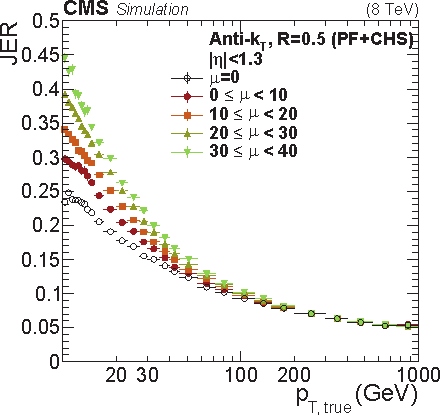
\includegraphics[width=0.49\textwidth]{figures/reconstruction/jer_res.pdf}}\hspace{0.03\textwidth}
\subfloat[\label{fig:reconstruction-jer-sf}]{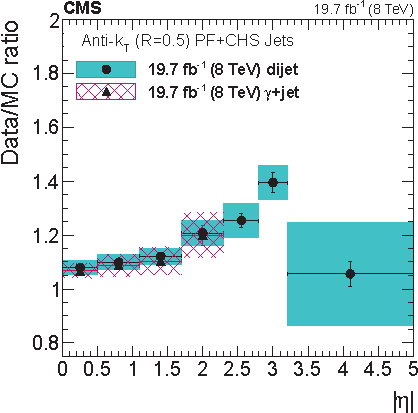
\includegraphics[width=0.47\textwidth]{figures/reconstruction/jer_sf.pdf}}
}



%##############################################
\section{b-tagging}
%##############################################
\label{sec:reconstruction-btagging}

The identification of jets that stem from the hadronization of b~quarks, so-called ``b-tagging'', is a crucial ingredient in studies of top quark production. It provides discrimination power to single out jets which can be related to b~quarks as expected in top quark decays.

Multiple algorithms have been developed within \gls{cms} to perform b-tagging~\cite{Chatrchyan:2012jua,CMS-PAS-BTV-15-001} for jets that fall within the pseudorapidity acceptance of the tracker. A common feature of most algorithms is the identification of a secondary vertex which is reconstructed from displaced tracks within a jet. The general idea is illustrated in Fig.~\ref{fig:reconstruction-btagging}. After hadronization, a final state b~quark is encapsulated into a B~meson~(e.g. $\mathrm{B}^{\pm}$, $\mathrm{B}_{0}$, $\mathrm{B}_\mathrm{s}$) which can then travel a measurable distance away from the primary vertex before decaying due to its relatively long lifetime. For example, a $\mathrm{B}^{\pm}$~meson, which has a mean lifetime of about $1.6~\mathrm{ps}$~\cite{Olive:2016xmw}, can travel distances of roughly $4\range9~\mathrm{mm}$ for momenta of $40\range100~\GeV$ on average before decaying.

\myfigure{\label{fig:reconstruction-btagging} Sketch of the production of displaced tracks in b~jets through the displaced decay of a B~hadron.}{
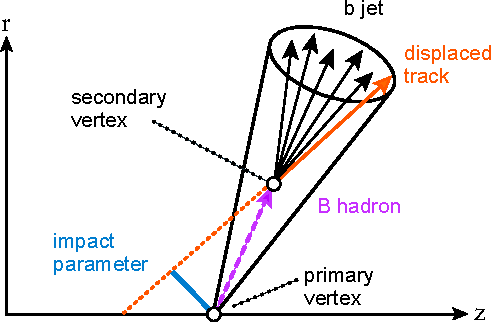
\includegraphics[scale=0.65]{figures/reconstruction/btagging.pdf}
}

After reconstruction, secondary vertices are subjected to pass certain quality criteria to enhance their purity with respect to the B~meson hypothesis. These are based on the amount of shared tracks with the primary vertex, the invariant vertex mass to reject kaon decays, and the direction of tracks with respect to the jet axis. In this thesis, b-tagging algorithms based on multivariate discriminators are employed. These combine multiple properties of the secondary vertex, tracks, and impact parameters amongst others into a powerful discriminant. The training of the discriminator also covers scenarios where no secondary vertex has been reconstructed within a jet. In such cases, the compatibility of tracks with the primary vertex is condensed into the discriminant. A comparison of the performance of various b-tagging algorithms employed within \gls{cms} is presented in Fig.~\ref{fig:reconstruction-btagging-algo}. It shows the misidentification probability of falsely tagging charm and light~(g,u,d,s) quarks as a function of the efficiency to identify true b~jets in simulation.

\myfigure{\label{fig:reconstruction-btagging-algo}Comparison of various b-tagging algorithms in simulation. The indicated version~2 refers to the algorithms in Run~2. The figure is taken from Ref.~\cite{CMS-PAS-BTV-15-001}.}{
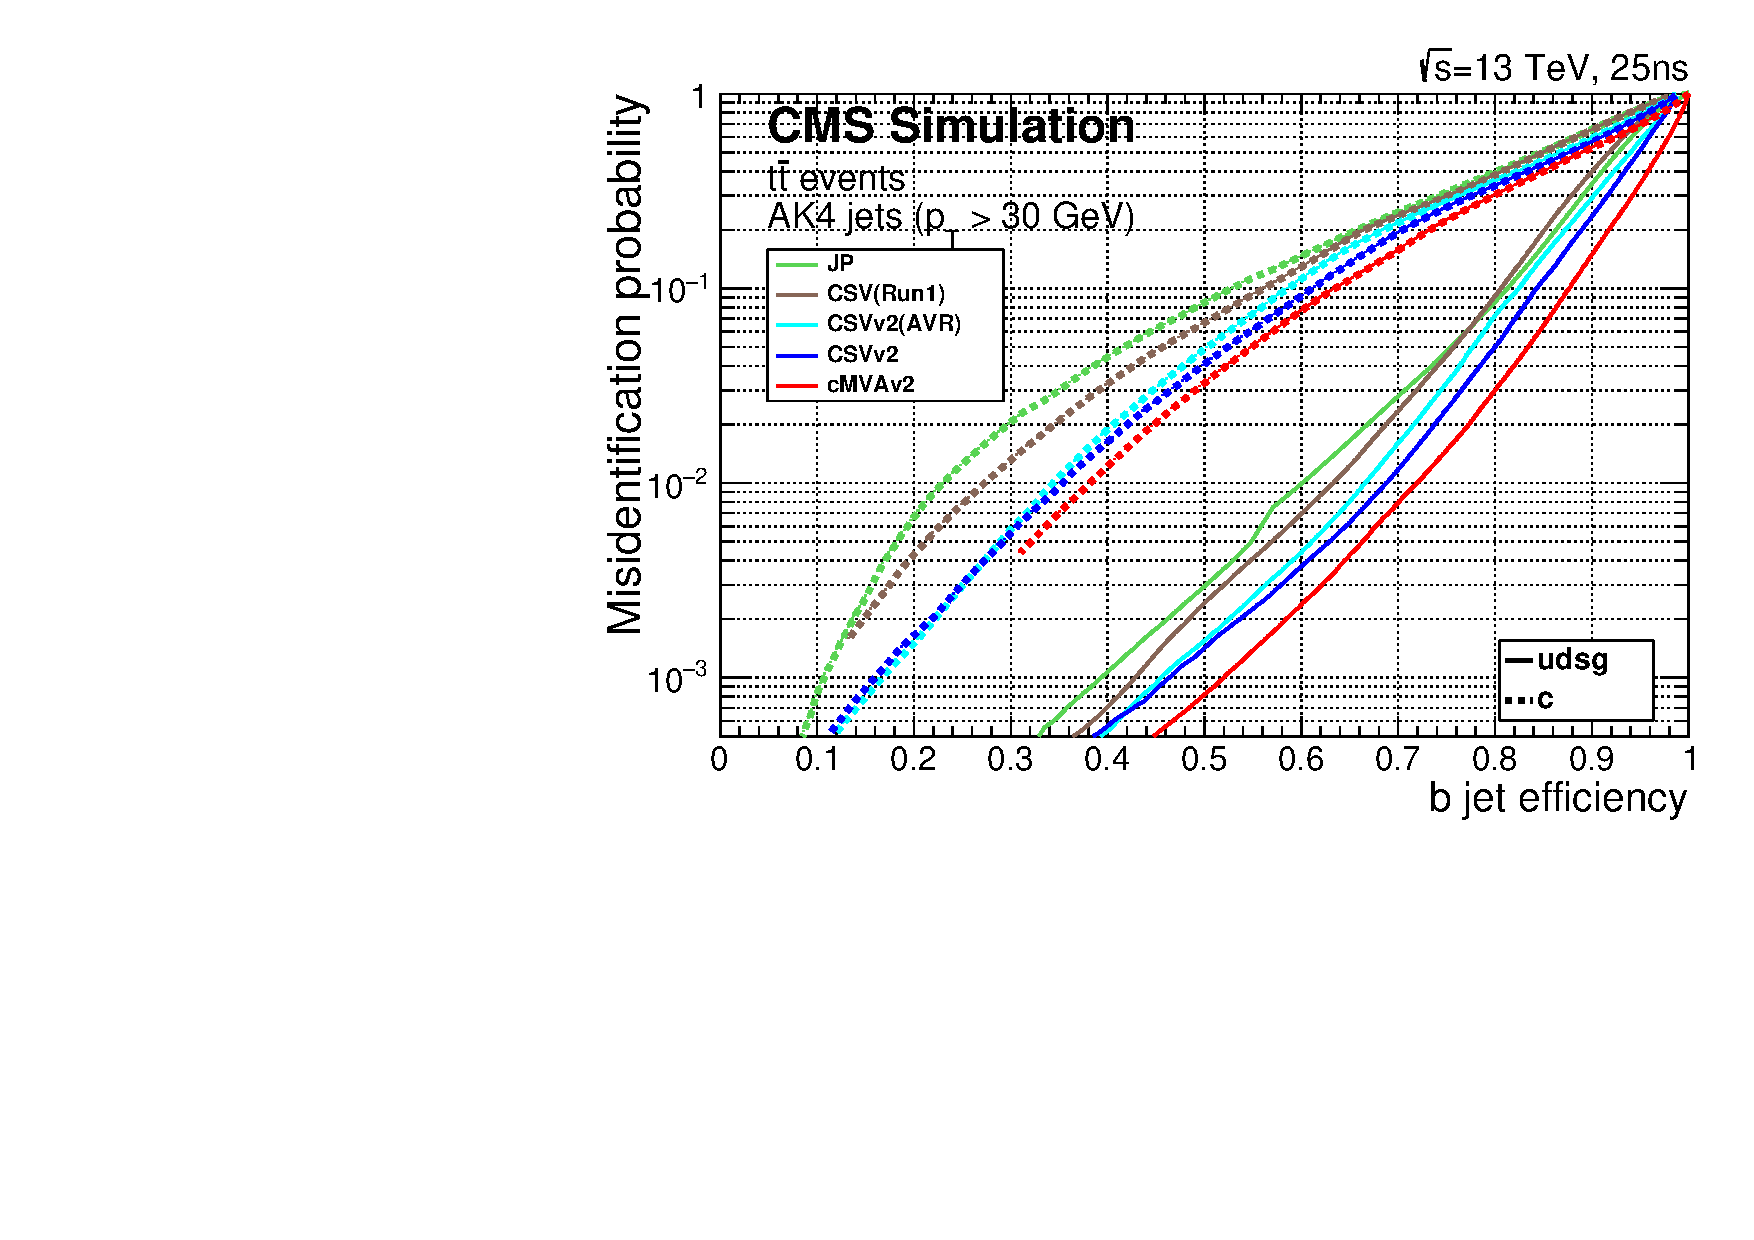
\includegraphics[width=0.7\textwidth]{figures/reconstruction/btag_comparison.pdf}\hspace{0.1\textwidth}
}

The \glshere{csv} (Run~1) algorithm is employed in the 8~TeV and first 13~TeV (\gls{csv} version~2) analyses within this thesis. At their tight working points, a b-tagging efficiency of approximately 50\% with a misidentification probability of only 0.1\% is achieved. A new algorithm, called \glshere{cmva}, is utilized in the analysis of 13~TeV data recorded in 2016. It combines the output of various other b-tagging algorithms which includes also the \gls{csv} discriminant. Additionally, the results of \gls{mva} discriminators trained to identify low-$\pt$ electrons or muons inside a jet for b-tagging are taken as inputs as well. The final \gls{cmva} discriminant exhibits an improved rejection of charm and light quark jets compared to the other algorithms as shown in Fig.~\ref{fig:reconstruction-btagging-algo}~\cite{CMS-PAS-BTV-15-001}.

The b-tagging efficiency in simulation typically deviates somewhat from the one observed in data. This is corrected by applying efficiency scale factors $\epsilon_\mathrm{b}^\mathrm{data}/\epsilon_\mathrm{b}^\mathrm{sim.}$ to simulation which are derived from data. Multiple methods are used to measure the scale factors in either multijet data events, which are enriched with heavy-flavored jets by requiring close-by muons, or in events with two leptons and two jets yielding a $\ttbar$-enriched sample~\cite{CMS-PAS-BTV-13-001}. A weight is calculated for each simulated jet based on the ratio of probabilities between simulation and data that the jet was tagged, i.e. its b-tagging discriminator value is past a working point. For multiple working points the weight can be expressed as

\begin{align}
w^\mathrm{jet}=\frac{p_\mathrm{data}\big(\mathrm{jet}\,\big|~W_{i}<d^\mathrm{jet}<W_{i+1}\big)}{p_\mathrm{sim.}\big(\mathrm{jet}\,\big|~W_{i}<d^\mathrm{jet}<W_{i+1}\big)}
=\frac{
s^\mathrm{jet}_{i}\cdot\epsilon^\mathrm{jet}_{i}-s^\mathrm{jet}_{i+1}\cdot\epsilon^\mathrm{jet}_{i+1}}{\epsilon^\mathrm{jet}_{i}-\epsilon^\mathrm{jet}_{i+1}}\,,
\end{align}

where $d^\mathrm{jet}$ denotes the value of the b-tagging discriminant, $W_{i}$ the working points $i=0\ldots N$, $\epsilon_i$ the efficiency measured in simulation, and $s_i$ the corresponding scale factors. In this equation, the scale factors and efficiencies for untagged jets ($i=0$) are set to $s_{0}=\epsilon_{0}=1$ whereas the efficiency of passing the highest working point $W_N$ is set to $\epsilon_{N+1}=0$. An event is reweighted by the multiplied weights from all jets passing the selection. The efficiencies and scale factors themselves depend on the reconstructed jet $\pt$, $\eta$ and flavor, where the latter is determined from the decay and hadronization history of a matched true jet. In case no true jet can be matched (e.g. the reconstructed jet is driven by \gls{pf} candidates from pileup interactions) a light flavored quark~(g,u,d,s) is assumed as its origin.



 
%##############################################
\section{Missing transverse energy}
%##############################################

The missing transverse momentum, \pvmiss, and energy, \met, is calculated from the momentum imbalance of the summed \gls{pf} candidate momenta as

\begin{equation}
\met=|\pvmiss|\,,\qquad \pvmiss=\colvec{2}{\pvmissx}{\pvmissy}=-\sum_{i}^\mathrm{\gls{pf}~cand.}\vec{p}_{\mathrm{T},i}\,.
\end{equation}

In analyses it can be used to infer the summed transverse momenta of produced neutrinos which escape the \gls{cms} detector without being detected due to their very low interaction probability. In this thesis one neutrino is expected to be produced in signal events stemming from the decay of a single top quark which can lead to significant missing transverse energy of about $\langle\met\rangle\approx50~\GeV$ on average. The $\pvmissz$ component cannot be calculated from the momentum imbalance since the boost along the z-axis of an event, determined by the initial parton momentum fractions $x_i$, cannot be reconstructed.

The \met scale is improved by propagating the corrected energy for \gls{pf} candidates which are clustered into jets to the missing transverse momentum. Only jets with a $\pt$ of at least $10~\GeV$ ($15~\GeV$) are considered for which energy calibrations are measured in 8~\TeV (13~\TeV) data respectively. The correction can be expressed as

\begin{subequations}
\begin{align}
\pvmiss^\mathrm{corr.}&=-~\sum_{i}^\mathrm{jets}~\vec{p}_{\mathrm{T},i}^\mathrm{\,corr.}~~-\sum_{i}^\mathrm{unclustered}\vec{p}_{\mathrm{T},i}^\mathrm{\,raw}\\
&=\pvmiss^\mathrm{raw}-~\sum_{i}^\mathrm{jets}\left(\, \vec{p}_{\mathrm{T},i}^\mathrm{\,full~\gls{jec}}~-~\vec{p}_{\mathrm{T},i}^\mathrm{\,\gls{pu}\mbox{-}only}\right)\,,
\end{align}
\end{subequations}

where $\vec{p}_{\mathrm{T},i}^\scriptn{\mathrm{\,\gls{pu}\mbox{-}only}}$ denotes the transverse jet momentum after applying only the first level of energy corrections which deals with the contribution from pileup. The resulting improvement is demonstrated in Fig.~\ref{fig:reconstruction-met}. It shows the parallel component of the missing momentum vector $u_{\parallel}$ along the direction of a reconstructed $\mathrm{Z}$~boson or photon $\vec{q}_\mathrm{T}$ in a ratio over the recoil momentum. After propagating the applied jet energy corrections to \pvmiss, the energy scale of its parallel component is reconstructed well within 3\% or better for recoil momenta above $50~\GeV$. At low momenta, contributions from unclustered \gls{pf} candidates dominate which results in a degradation of the energy scale.

\myfigure{\label{fig:reconstruction-met}The average $\pvmiss$ component parallel to the recoiling $\mathrm{Z}/\gamma$ boson as a function of the boson's momentum. The figure is taken from Ref.~\cite{CMS-PAS-JME-12-002}.}{
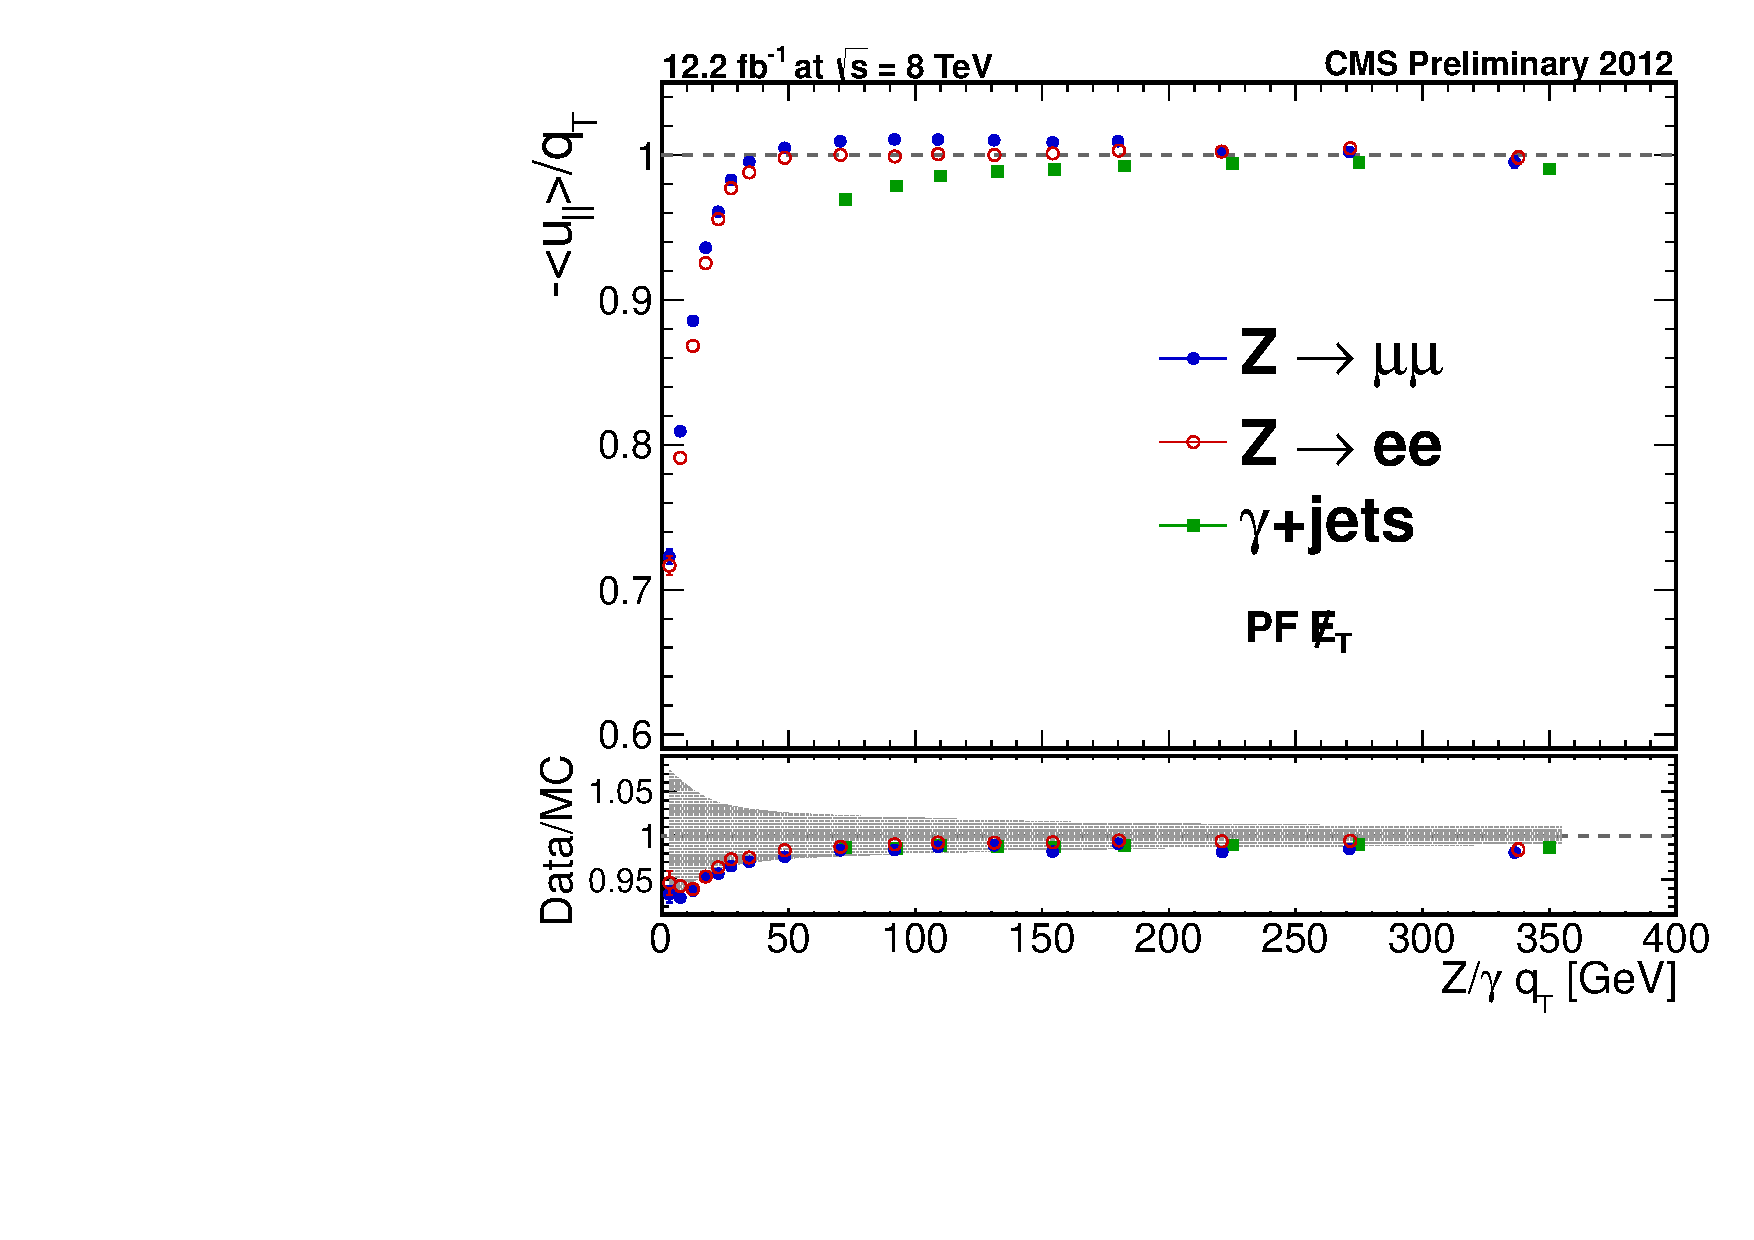
\includegraphics[width=0.5\textwidth]{figures/reconstruction/met_recoil.pdf}
}

In 8~TeV data and simulation an additional correction is applied to decrease the influence of pileup on the \met scale. Since typical inelastic \gls{pp} interactions do not produce any prompt neutrinos, pileup events will only lead to a smearing of the \met due to the finite detector response for measuring neutral particle momenta. This can be mitigated by subtracting the amount of charged and neutral energy associated to pileup vertices where the latter is estimated from the amount of charged hadron activity.


%##############################################
\section{Luminosity}
%##############################################

The luminosity delivered by the \gls{lhc} during collisions at the \gls{cms} interaction point is determined by measuring certain process rates with so-called luminometers. These are the pixel detector, the \gls{hf} calorimeter, and the pixel luminosity telescope~\cite{Kornmayer:2039978} amongst others. The instantaneous luminosity is then calculated from the recorded process rate $R$ of the luminometer as

\begin{equation}
L\cdot\mathrm{d}t=\frac{R\cdot\mathrm{d}t}{\sigma_\mathrm{fid.}}\,,
\end{equation}

where $\sigma_\mathrm{fid.}=\sigma\cdot A$ is the fiducial cross section observed within the luminometer acceptance $A$. The fiducial cross section is estimated from so-called \glshere{vdm} scans during which the proton beams are first separated and then gradually crossed with each other. By fitting the rate as a function of the beam separation in such scans an absolute calibration of the luminometers is obtained. The most precise luminosity estimations for the data analyzed in this thesis are obtained with the pixel cluster counting method~\cite{CMS-PAS-LUM-13-001,CMS-PAS-LUM-15-001,CMS-PAS-LUM-17-001}. Here, the rate is defined as the number of pixel clusters reconstructed in the second and third pixel barrel layers per bunch crossing. This luminometer profits from the low channel occupancy of the pixel detector which results in a linear dependency between the cluster rate and the instantaneous luminosity even in high pileup events with many particle tracks.

From the measured luminosity the distribution of the number of pileup interactions in data can be inferred. For simulated samples a predefined distribution is assumed instead according which the hard scattering event is overlaid with additional minimum bias events. Thus, a reweighting of simulated events has to be performed to match the corresponding distribution of \gls{pu} interactions in data. 
The average number of \gls{pu} interactions is estimated in data per luminosity section using $\langle N_\mathrm{\gls{pu}}\rangle=\sigma_\mathrm{\gls{pp}}\cdot L$ where $\sigma_\mathrm{\gls{pp}}$ denotes the total inelastic \gls{pp} cross section. An event weight is then derived from the ratio of the distributions of \gls{pu} interactions in data and simulation. The inelastic cross section has been measured in 13~TeV \gls{pp} collisions as $71.3\pm3.5~\mathrm{mb}$~\cite{CMS-PAS-FSQ-15-005}. However, a better agreement between data and simulation is obtained for pileup sensitive observables such as the number of primary vertices or the median of the transverse energy density, $\rho$, with a slightly lower cross section of $69~\mathrm{mb}$.


%##############################################
\section{Summary of corrections}
%##############################################
\label{sec:reconstruction-summary}

Several corrections have been introduced throughout this chapter to improve the agreement between data and simulation. The corrections are also considered sources of systematic uncertainties in the presented analyses within this thesis. A summary of the corrections and associated uncertainties is provided in the following.

\begin{description}
\item[Lepton selection] The efficiencies for selecting isolated muons or electrons which pass dedicated tight identification criteria are corrected through data-to-simulation scale factors. In addition, the analyzed data events have been recorded using single muon or electron triggers whose efficiencies in simulation are also corrected to match the ones observed in data. The applied lepton scale factors are varied independently within one standard deviation of their measured uncertainties to assess the systematic impact on the measurements.
\item[Jet energy scale and resolution] The momenta of reconstructed jets in data and simulation are corrected to relate to the expected true jet energy derived from the hadronization products of partons in simulation. Residual corrections and a smearing procedure are applied to match the overall scale and resolution of the jet energy in data. The corrections are also propagated to the \met which improves its energy response as well. The systematic uncertainties arising from the measured energy and resolutions scale factors are estimated by varying them within their uncertainties and repeating the measurements with recalibrated jets and \met.
\item[Unclustered energy] The momentum of \gls{pf} candidates which are not clustered into jets is varied to estimate the uncertainty due their uncalibrated contributions to the missing transverse energy.
\item[B-tagging] Scale factors are applied in simulation to match the performance of the employed b-tagging algorithm in data. The systematic uncertainties are assessed for b and c~jets by varying their scale factors simultaneously while the scale factor for mistagging g,u,d,s~jets is varied independently.
\item[Pileup] The impact of pileup is estimated by varying the inelastic \gls{pp} cross section by $\pm5\%$ which changes the estimated distribution of true pileup interactions in data. The corresponding reweighting factors are rederived and applied to simulation.
\end{description}


%\chapter{Methodology of analyses techniques}
%\chapter{Polarization of single top quarks in \textsl{t}~channel at 8~TeV}

\intro{A first measurement of the top quark spin asymmetry in t~channel, sensitive to the top quark polarization, is presented in this chapter. Proton-proton collision data at $\mathit{\sqrt{s}=8}$~TeV have been analyzed corresponding to about $\mathit{20~fb^{-1}}$. Events with an isolated muon are selected together with two or three jets for the final measurement. Events containing an isolated electron and jets have been studied as well. The normalized differential cross section is measured as a function of the polarization angle. From its shape, a spin asymmetry of $\mathit{0.26\pm0.03~(stat)\pm0.10~(syst)}$ is obtained. This is found to be compatible within $\mathit{2.0}$ standard deviations with the expected \gls{sm} spin asymmetry of $\mathit{0.44}$. The result has been published in Ref.~\cite{Khachatryan:2015dzz}. In a further step, the derivation of limits on anomalous couplings is illustrated by combining the result of this measurement with related ones.}


An overview of the strategy to measure the top quark spin asymmetry and derive limits on anomalous couplings is given in the following. After selecting events with an isolated muon or electron and two or three jets, two \glspl{bdt} are employed. The first one, \bdtqcd, is trained to reject events with fake leptons stemming from multijet production. The shape of multijet production is modeled by a template obtained from data in a sideband region for which the lepton isolation is inverted. Then, a two-component \gls{ml} fit to the \bdtqcd discriminant is performed to estimate the amount of multijet contamination after the event selection. The second \gls{bdt}, \bdttch, is optimized to separate signal from \wjets and \ttbar events. The amount of signal and background contributions is estimated through a second \gls{ml} fit to its discriminant. A signal-enriched phase space is obtained by applying an optimized selection on each of the \gls{bdt} discriminants resulting in a \gls{sb} ratio of about 90\%. The shape of the polarization angle, $\cos\theta^\star_{\mu}$, in data is unfolded to parton level after subtracting the remaining background contributions. This is repeated for each considered source of systematic uncertainty to estimate their impact on the measurement. The final measurement is performed in the muon channel only since in the electron channel, shortcomings in the modeling of the data-driven multijet template and an overall larger impact of systematic uncertainties are observed rendering its standalone result much less significant. The following description of the analysis is therefore primarily focused on the muon channel. 

The spin asymmetry is obtained from the differential cross section through a linear fit. The \TOPFIT program is utilized in a further step to set limits on anomalous Wtb couplings by combining the measured spin asymmetry with an inclusive cross section measurement in $t$~channel and a measurement of the W~boson helicity fractions in \ttbar production.



%##############################################
\section{Event selection and simulated samples}
%##############################################
\label{sec:polarization-selection}

Proton-proton collision data at $\sqrt{s}=8~\TeV$ are analyzed corresponding to $19.7~\invfb$ recorded with the \gls{cms} experiment in 2012. Events are triggered on the presence of a single muon or electron candidate. The employed single muon trigger requires an isolated muon candidate with $\pt>24~\GeV$ within the pseudorapidity range of $|\eta|<2.1$. The single electron trigger fires when an electron candidate with $\pt>27~\GeV$ within $|\eta|<2.5$ is detected that has to fulfill some additional quality criteria which correspond to an efficiency of 80\% for prompt electrons. Events are categorized into ``channels'' depending whether they have been triggered with the muon or electron trigger. For analysis, events in the muon channel have to contain one muon candidate with $\pt>26~\GeV$ within $|\eta|<2.1$ that passes the tight identification requirements. In the electron channel, events considered for analysis have to contain one electron candidate with $\pt>30~\GeV$ within $|\eta|<2.5$ where however the \gls{ecal} barrel-endcap transition region is excluded. In addition, the electron candidate has to fulfill the tight \gls{mva}-based identification requirements. To suppress fake leptons from multijet production, the muon candidate is required to be isolated with a relative \gls{deltabeta}-based isolation of $\muiso<12\%$ whereas the electron candidate has to have a relative \gls{effarea}-based isolation of $\eiso<10\%$. Events containing additional muons~($\pt>10~\GeV$, $|\eta|<2.5$, $\muiso<20\%$) or electrons~($\pt>20~\GeV$, $|\eta|<2.5$, $\eiso<15\%$) which pass corresponding loose identification criteria are rejected to suppress contributions from \zjets and dileptonic \ttbar production. 

Jets are clustered from \gls{pf} candidates with the anti-\kt algorithm using a distance parameter of $R=0.5$ while applying the \gls{chs} technique to remove the contamination of pileup tracks. \gls{pf} candidates belonging to preselected muons or electrons with a loose isolation are not clustered into the jets to prevent double counting. In addition, jets which are within $\Delta R<0.3$ to the selected tight lepton are ignored in the analysis. The reconstructed jet energy in data and simulation and the energy resolution in simulation are calibrated through dedicated \gls{jec} and \gls{jer} scale factors. Events containing in addition to a tight lepton two or three jets with $\pt>40~\GeV$ within $|\eta|<4.5$ that pass loss identification criteria are considered for analysis. B-tagging of jets is performed with the \gls{mva}-based \gls{csv} algorithm. The tagging of jets is restricted to $|\eta|<2.4$ since the algorithm operates only within the acceptance of the inner tracking system. In simulation an efficiency of about 50\% for tagging true b~jets with a mistagging rate of 0.1\% for other jets is found at the employed tight working point of the algorithm. The b-tagging efficiency is reweighted in simulation through scale factors to match the one measured in data. More details about the analysis objects, identification, and corrections have been described in Ch.~\ref{ch:reconstruction}.

After the selection, events are categorized per lepton channel as visualized in Fig.~\ref{fig:polarization-categorization}. The regions are labeled as ``$N\,\mathrm{j}~M\,\mathrm{t}$'' where $N$ denotes the number of selected jets and $M$ the subset of jets which are also b-tagged. Control regions dominated by either \wjets~(2j0t) or \ttbar~(3j1t, 3j2t) production are defined besides the signal region~(2j1t) as indicated in Fig.~\ref{fig:polarization-categorization}. The analysis was developed by validating the background modeling and optimizing the strategy using data in the control regions only. During this process, distributions of data in the signal region have not been used which is commonly referred to as ``blinding''. After the strategy is fixed the final measurement was conducted by unblinding the signal region while refraining from any further optimizations. Thus, the blinding procedure prevents a result-driven tuning of the analysis strategy which may otherwise bias the result.

\myfigure{\label{fig:polarization-categorization}Categorization of events depending on number of selected jets, number of b-tags, and the signal \gls{bdt} discriminant. The shaded regions are utilized in a template-based \gls{ml} fit as described in Sec.~\ref{sec:polarization-fit} for estimating the signal and background yields.}{
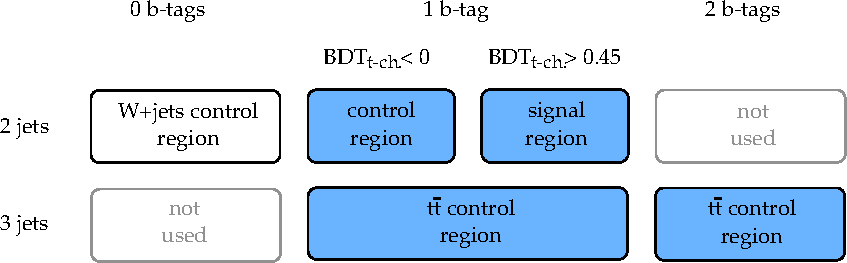
\includegraphics[scale=0.75]{figures/polarization/regions.pdf}
}

Various samples of simulated events for signal and background processes are generated. The default $t$-channel single-top-quark signal sample is generated in 5~\gls{fs} using the \POWHEG\,v1 generator interfaced with \PYTHIA\,6 for parton showering and \TAUOLA for tau decays. For comparisons, two additional, alternative signal samples are generated. One utilizes the \AMC generator interfaced with \PYTHIA\,8 in 4~\gls{fs} while the other employs the \COMPHEP generator interfaced with \PYTHIA\,6. A set of special samples with anomalous Wtb couplings is generated as well using the \COMPHEP generator for cross checking the analysis strategy. Samples containing single top quark events produced via tW and $s$~channel are generated with \POWHEG\,v1 interfaced with \PYTHIA\,6 and \TAUOLA. The major background processes, \wjets, \zjets, and \ttbar, are generated with the \MG generator interfaced with \PYTHIA\,6 and \TAUOLA as well. Samples with up to three~(\ttbar) or four~(\wjets,\zjets) additional partons at \gls{me} level are merged together using the \gls{mlm} procedure. For \wjets production, an alternative sample generated with the \SHERPA generator~\cite{Hoeche:2012ft} is employed for validation purposes. In this thesis, \wjets events are categorized based on their jet flavor content. Events with at least one heavy-quark flavored jet from either c, or b~quarks are abbreviated as ``\glsmark{whf}'' while events with only light-quark flavored jets~(g,u,d,s) are labeled as ``\glsmark{wlf}'' instead. Diboson production~(WW,WZ,ZZ) is a minor background and simulated with \PYTHIA\,6. The theoretical \gls{sm} cross sections used to normalize the samples are listed in Tab.~\ref{tab:polarization-theo-xsecs}. Throughout this chapter the individual signal and background templates are shown after they have been scaled to the result of a binned \gls{ml} fit to data~(Sec.~\ref{sec:polarization-fit}) and corrections to the simulated \wjets and \ttbar events~(Sec.~\ref{sec:polarization-modeling}) have been applied unless explicitly stated otherwise.


\mytable{\label{tab:polarization-theo-xsecs}Theoretical cross sections used to normalize the simulated samples.}{
\begin{tabular}{|l  r c l |}
\hline
process & $\sigma/\pb$ &\hspace{0.1cm} & accuracy \\
\hline
$t$~channel & $87.1~\pb$ & & approx. \gls{nnlo}~\cite{Kidonakis:2012db} \\
$s$~channel & $5.55~\pb$ && approx. \gls{nnlo}~\cite{Kidonakis:2012db}  \\
tW~channel & $22.2~\pb$ && approx. \gls{nnlo}~\cite{Kidonakis:2012db} \\
\ttbar & $252.9~\pb$ && \gls{nnlo} (using Top++\,2.0~\cite{Czakon:2011xx}) \\
$\mathrm{W}\to\ell\nu\mathrm{\,\mbox{+}\,jets}$ & $37\,509~\pb$ && \gls{nnlo} (using FEWZ~\cite{Gavin:2010az}) \\
$\mathrm{Z}/\gamma^{*}\to\ell^{\rmplus}\ell^{\rmminus}$, $m_{\ell\ell}>50~\GeV$ & $3\,504~\pb$ && \gls{nnlo} (using FEWZ~\cite{Gavin:2010az}) \\
WW & $54.8~\pb$ && \gls{nlo} (using MCFM\,5.8~\cite{Campbell:2010ff})\\
WZ & $33.2~\pb$ && \gls{nlo} (using MCFM\,5.8~\cite{Campbell:2010ff})\\
ZZ & $8.1~\pb$ && \gls{nlo} (using MCFM\,5.8~\cite{Campbell:2010ff})\\
\hline
\end{tabular}
}

Contributions from fake leptons produced in multijet events that survive the event selection are not simulated but estimated from data through the following procedure. The shape of multijet events per channel is extracted from a sideband region for which the isolation of the lepton is inverted in the event selection as $\muiso>20\%$ and $\eiso>15\%$, respectively. The resulting distribution of data after subtracting the remaining contamination by other processes serves as a template to model the shape of multijet production per observable. The amount of multijet production in signal and control regions is estimated by fitting the extracted template to data. The fit setup is described later in Sec.~\ref{sec:polarization-fit}. Figure~\ref{fig:polarization-qcd-template-antiiso} shows the distribution of the transverse W~boson mass in the 2j1t sideband region of the muon channel. The contribution of other processes in the sideband region amounts to a contamination of only 9\% (2\%) in muon (electron) channel respectively. The resulting multijet template after it has been fitted to data in the 2j1t region of the muon channel is shown in Fig.~\ref{fig:polarization-qcd-template-iso}. The data-driven procedure yields a good description of the unknown multijet shape in the signal region here.

\myfigure{\label{fig:polarization-qcd-template}Distributions of the transverse W~boson mass in muon channel: (a)~antiisolated sideband region for extracting the multijet template; (b)~resulting distribution in the 2j1t region after scaling the extracted template to data through a \gls{ml} fit.}{
\subfloat[\label{fig:polarization-qcd-template-antiiso}]{\adjincludegraphics[height=4.8cm,trim={0 0 {0.16\width} 0},clip]{figures/polarization/beforeBgCorr/2j1t/muon_2j1t_mtw_qcdnone_antiiso_nol.pdf}}
\subfloat[\label{fig:polarization-qcd-template-iso}]{\adjincludegraphics[height=4.8cm,trim={0 0 {0.\width} 0},clip]{figures/polarization/afterBgCorr/2j1t/muon_2j1t_mtw_qcdnone.pdf}}
}

Distributions of the reconstructed top quark mass in muon and electron channel are presented in Fig.~\ref{fig:polarization-topmass} after the event selection and the estimation of multijet events have been performed. In control regions containing no or more than one b-tagged jet, the jet with the highest value of the \gls{csv} discriminant is associated to the top quark decay to calculate the top quark mass.  The presented distributions demonstrate that data is well described by the simulated event samples and the data-driven multijet templates in control and signal regions for electron and muon channel.

In a top quark mass range of about $150\range190~\GeV$ the distributions display a peak for single top quark production as expected. For \ttbar production, the selected b-tagged jet may not be always associated with the corresponding lepton from a top quark decay. Hence, its distributions results into a peak with a wider tail. Unfortunately, the event selection also leads to a similar peak-like shape for the \wjets background although with an even longer tail. From these distributions it can be concluded that a simple selection on the top quark mass is insufficient to select a signal-enriched phase space. Therefore, two \glspl{bdt} are trained for separating signal from background events more efficiently as detailed in the next section.

\myfigure[p]{\label{fig:polarization-topmass} Distributions of the reconstructed top quark mass in (left column)~electron and (right column)~muon channel. Top row: 2j0t \wjets control region; middle row: 2j1t region; bottom row: 3j1t \ttbar control region. The top quark \pt reweighting~(Sec.~\ref{sec:polarization-modeling}) is exceptionally not applied here.}{
\subfloat[]{\adjincludegraphics[height=4.8cm,trim={0 0 {0.16\width} 0},clip]{figures/polarization/beforeBgCorr/2j0t/electron_2j0t_top_mass_qcdnone_nol.pdf}}
\subfloat[]{\adjincludegraphics[height=4.8cm,trim={0 0 {0.\width} 0},clip]{figures/polarization/beforeBgCorr/2j0t/muon_2j0t_top_mass_qcdnone.pdf}}\\
\subfloat[]{\adjincludegraphics[height=4.8cm,trim={0 0 {0.16\width} 0},clip]{figures/polarization/beforeBgCorr/2j1t/electron_2j1t_top_mass_qcdnone_nol.pdf}}
\subfloat[]{\adjincludegraphics[height=4.8cm,trim={0 0 {0.\width} 0},clip]{figures/polarization/beforeBgCorr/2j1t/muon_2j1t_top_mass_qcdnone.pdf}}\\
\subfloat[]{\adjincludegraphics[height=4.8cm,trim={0 0 {0.16\width} 0},clip]{figures/polarization/beforeBgCorr/3j2t/electron_3j2t_top_mass_qcdnone_nol.pdf}}
\subfloat[]{\adjincludegraphics[height=4.8cm,trim={0 0 {0.\width} 0},clip]{figures/polarization/beforeBgCorr/3j2t/muon_3j2t_top_mass_qcdnone.pdf}}
}



%##############################################
\section{Training of Boosted Decision Trees}
%##############################################
\label{sec:polarization-bdt-training}

Two \glspl{bdt} are trained to obtain a signal-enriched phase space. The first \gls{bdt}, labeled \bdtqcd, is trained to reject background events stemming from multijet production. Simulated $t$-channel single top quark events are set as signal class and data events from the sideband region where the multijet template is extracted are set as background class. The gradient boosting procedure is chosen for the training with a relatively low shrinkage of 10\%. The number of single decision trees is restricted to 50 while each tree is kept shallow with a maximum depth of two. The minimum node size is set to 250 events. These settings are not optimized to yield the best discrimination power but instead are motivated to protect well against overtraining. This a particular concern here since the usage of data events for training may not reflect the distribution of multijet events in the signal region to the extend as it would be with simulated events. Multiple \gls{bdt} candidates are trained to assess which set of discriminating input observables yields the best rejection of multijet events with the final discriminant. Correlated observables are excluded from the training by testing individually that the discrimination power does not diminish when removed. This resulted in the following list of five input observables:

\begin{itemize}
\item the reconstructed invariant mass of the top quark candidate;
\item the transverse mass of the W~boson candidate before solving for the unknown neutrino $p_{z}$ component since this modifies \pvmiss in case of complex solutions, \mtw;
\item the missing transverse energy, \met;
\item the transverse momentum of the untagged spectator jet~(\jprime);
\item the event isotropy which is defined as $(s_\mathrm{max}-s_\mathrm{min})/s_\mathrm{max}$ with $s=\sum_{i}^\scriptn{\ell,\,\mathrm{jets}}\big|\,\vec{n}\cdot\vec{p}_{i}\big|$ where the unit vector $\vec{n}=(\cos\phi,\sin\phi)$ is chosen in the transverse plane such that it either maximizes or minimizes $s$.
\end{itemize}

Distributions of \mtw, $\jprime~\pt$, and the event isotropy are presented in Fig.~\ref{fig:polarization-qcdinputs} while the other input observables are shown in Figs.~\ref{fig:polarization-qcd-template} and~\ref{fig:polarization-topmass} above. The distribution of the resulting \gls{bdt} discriminant is shown Fig.~\ref{fig:polarization-bdt-qcd}. A fair agreement is observed between data and simulation.

\myfigure{\label{fig:polarization-qcdinputs}Distributions of some input observables of the \bdtqcd and \bdttch discriminants as indicated in 2j1t muon channel: (a)~missing transverse energy; (b)~transverse momentum of untagged spectator jet; (c)~event isotropy; (d)~transverse momentum of b~tagged jet.}{
\subfloat[\bdtqcd and \bdttch]{\adjincludegraphics[height=4.8cm,trim={0 0 {0.16\width} 0},clip]{figures/polarization/afterBgCorr/2j1t/muon_2j1t_met_qcdnone_nol.pdf}}
\subfloat[\bdtqcd and \bdttch]{\adjincludegraphics[height=4.8cm,trim={0 0 {0.\width} 0},clip]{figures/polarization/afterBgCorr/2j1t/muon_2j1t_ljet_pt_qcdnone.pdf}}\\
\subfloat[only \bdtqcd]{\adjincludegraphics[height=4.8cm,trim={0 0 {0.16\width} 0},clip]{figures/polarization/afterBgCorr/2j1t/muon_2j1t_isotropy_qcdnone_nol.pdf}}
\subfloat[only \bdttch]{\adjincludegraphics[height=4.8cm,trim={0 0 {0.\width} 0},clip]{figures/polarization/afterBgCorr/2j1t/muon_2j1t_bjet_pt_qcdnone.pdf}}
}

In a preliminary version of this analysis~\cite{CMS-PAS-TOP-13-001}, events with $\mtw>50~\GeV$ ($\met>45~\GeV$) are selected in muon (electron) channel respectively to reject multijet events. Here, the working points of the \bdtqcd discriminant have been chosen such that similar signal selection efficiencies are obtained per channel. A comparison of the working point performances is presented in Tab.~\ref{tab:polarization-qcdeff}. The usage of the new \bdtqcd with respect to the preliminary analysis allows to reject about twice as much multijet events while retaining approximately the same amount of signal events.

\mytable{\label{tab:polarization-qcdeff}Selection efficiencies of multijet and signal events using \bdtqcd, \mtw, and \met working points where the latter two were used in a preliminary version of the analysis.}{
\begin{tabular}{|r | c c | c c |}
\hline
& \multicolumn{2}{c|}{Muon channel} & \multicolumn{2}{c|}{Electron channel}\\
Process    & $\mtw>50~\GeV$ & $\bdtqcd>-0.15$ & $\met>45~\GeV$ & $\bdtqcd>0.15$ \\
\hline
Multijet  & 15\% & 7.7\%  & 7.6\% & 4.4\% \\
Signal   & 70\% & 71\%   & 51\%  & 52\% \\
\hline
\end{tabular}
}

The second \gls{bdt}, \bdttch, is trained to separate signal events from \wjets and \ttbar production which are the major background processes after applying the multijet rejection selection. It is configured as follows. The gradient boosting method is employed with a shrinkage of 40\%. In total, 200~shallow single decision trees with a maximum depth of two are trained. The minimum node size is set to 100 events. To mitigate a potential lack in the training statistics of the backgrounds, additional simulated \wjets and \ttbar events from the 2j0t and 3j2t control regions are added to the training, respectively. In particular, this increases the statistics of W+light flavored jets which is relatively low in simulation in the 2j1t region but may in fact be larger in data due to mistagging. The following ten observables have been chosen as input:

\begin{itemize}
\item the reconstructed invariant mass of the top quark candidate;
\item the missing transverse energy, \met;
\item the transverse mass of the W~boson candidate before solving for the unknown neutrino $p_{z}$ component, \mtw;
\item the transverse momentum of the lepton;
\item the transverse momentum of the b-tagged jet;
\item the invariant mass of the b-tagged jet from the summed momenta of the clustered \gls{pf} candidates;
\item the absolute pseudorapidity of the untagged spectator jet~(\jprime);
\item the absolute pseudorapidity of the b-tagged jet;
\item the invariant mass of the top quark and spectator jet system, $\sqrt{\hat{s}}=\big|\vec{p}_{\mathrm{top}}+\vec{p}_{\jprime}\big|$\,;
\item the transverse momentum of the hadronic final-state system~(\glsmark{hfs}), $\big(\vec{p}_{\jprime}+\vec{p}_{\mathrm{b}}\big)_\mathrm{T}$\,.
\end{itemize}

These observables have been chosen because they exhibit a low correlation with the polarization angle. A bias may otherwise occur since the \gls{bdt} is trained with a sample of simulated signal events with a \gls{sm} coupling structure. In the worst case, the \gls{bdt} may select events in such a way that it artificially reproduces the shape of the expected polarization angle in data. Choosing uncorrelated observables makes the \gls{bdt} training blind to the actual distribution of the polarization angle instead. The distributions of some input observables are shown in Fig.~\ref{fig:polarization-tchinputs} after selecting events with $\bdtqcd>-0.15$ in 2j1t muon channel. The remaining ones are presented in Figs.~\ref{fig:polarization-qcd-template}, \ref{fig:polarization-topmass}, and~\ref{fig:polarization-qcdinputs} above. The resulting discriminant is shown in Fig.~\ref{fig:polarization-bdt-tch} in 2j1t muon channel. Overall, a good description of data with simulation is observed.

\myfigure{\label{fig:polarization-bdts}Distributions of the \glspl{bdt} discriminants in 2j1t muon channel: (a)~multijet \gls{bdt}; (b)~signal \gls{bdt} after rejecting multijet events.}{
\subfloat[\label{fig:polarization-bdt-qcd}]{\adjincludegraphics[height=4.8cm,trim={0 0 {0.16\width} 0},clip]{figures/polarization/afterBgCorr/2j1t/muon_2j1t_bdt_qcd_qcdnone_nol.pdf}}
\subfloat[\label{fig:polarization-bdt-tch}]{\adjincludegraphics[height=4.8cm]{figures/polarization/afterBgCorr/2j1t/muon_2j1t_bdt_tch_qcdbdt.pdf}}
}

\myfigure[p]{\label{fig:polarization-tchinputs}Distributions of some input observables to the \bdttch discriminant in 2j1t muon channel: (a)~transverse momentum of the muon; (b)~invariant mass of the b-tagged jet; (c,d)~absolute value of the untagged and b-tagged jet pseudorapidities; (e)~invariant mass of the top quark and spectator jet system; (f)~\pt of the hadronic final state system.}{
\subfloat[]{\adjincludegraphics[height=4.8cm,trim={0 0 {0.16\width} 0},clip]{figures/polarization/afterBgCorr/2j1t/muon_2j1t_lepton_pt_qcdbdt_nol.pdf}}
\subfloat[]{\adjincludegraphics[height=4.8cm,trim={0 0 {0.\width} 0},clip]{figures/polarization/afterBgCorr/2j1t/muon_2j1t_bjet_mass_qcdbdt.pdf}}\\
\subfloat[]{\adjincludegraphics[height=4.8cm,trim={0 0 {0.16\width} 0},clip]{figures/polarization/afterBgCorr/2j1t/muon_2j1t_ljet_abseta_qcdbdt_nol.pdf}}
\subfloat[]{\adjincludegraphics[height=4.8cm]{figures/polarization/afterBgCorr/2j1t/muon_2j1t_bjet_abseta_qcdbdt.pdf}}\\
\subfloat[]{\adjincludegraphics[height=4.8cm,trim={0 0 {0.16\width} 0},clip]{figures/polarization/afterBgCorr/2j1t/muon_2j1t_shat_mass_qcdbdt_nol.pdf}}
\subfloat[]{\adjincludegraphics[height=4.8cm,trim={0 0 {0.\width} 0},clip]{figures/polarization/afterBgCorr/2j1t/muon_2j1t_hfs_pt_qcdbdt.pdf}}
}


%##############################################
\section{Background modeling}
%##############################################
\label{sec:polarization-modeling}

The modeling of the \wjets and \ttbar backgrounds is studied in control regions before performing the measurement. In the 2j0t control region, two mismodeled observables are found which can be attributed to the \wjets background, after applying the \bdtqcd selection to reject the multijet background. 

The transverse momentum of the W~boson displays a softer spectrum in data compared to simulation as shown in Fig.~\ref{fig:polarization-wjets-reweighting-wpt}. This effect can be explained as an insufficient modeling of the hadronic recoil in such events. The recoil momentum is defined for \zjets and \wjets events as the net momentum which balances the momentum of the vector boson in the transverse plane. It is mostly the vectorial sum of hard jets but has also a soft contributions stemming from the underlying event, bremsstrahlung photons, and pileup. In this analysis, a simple reweighting of simulated events in bins of the W~boson \pt is applied to correct for this deviation. More sophisticated methods can be found in literature (e.g. Ref.~\cite{Abazov:2009tra}). The W~boson \pt scale factors derived in the 2j0t control region are also applied in the 2j1t signal region. In the statistical evaluation, the difference between applying and not applying this reweighting is considered as a systematic uncertainty.

\myfigure{\label{fig:polarization-wjets-pt}Distributions of the reconstructed W~boson \pt in 2j0t control region: (a)~before and (b)~after applying the \wjets corrections.}{
\subfloat[\label{fig:polarization-wjets-reweighting-wpt}]{\adjincludegraphics[height=4.8cm,trim={0 0 {0.16\width} 0},clip]{figures/polarization/beforeBgCorr/2j0t/muon_2j0t_wboson_pt_qcdbdt_nol.pdf}}
\subfloat[\label{fig:polarization-wjets-reweighting-wpt-rew}]{\adjincludegraphics[height=4.8cm,trim={0 0 {0.\width} 0},clip]{figures/polarization/afterBgCorr/2j0t/muon_2j0t_wboson_pt_qcdbdt.pdf}}
}

Another mismodeling of the \wjets background is observed for the polarization angle itself which is presented in Fig.~\ref{fig:polarization-wjets-reweighting-cosTheta}. This is a percuiliar mismodeling since $\cos\theta_\mu^\star$ does not reflect a physically meaningful observable for \wjets events. A similar deviation has been observed in measurements at 7~TeV as well~\cite{Komm-thesis}. The modeling is cross checked using an alternative \wjets sample simulated with the \SHERPA generator. This sample was however simulated with only massless quarks. Hence the ratio of light, charm, and bottom flavored jets is predicted wrongly. The flavor ratios are therefore reweighted to the ones predicted by the default \MG sample. The distributions before and after the reweighting are shown in Fig.~\ref{fig:polarization-sherpa-cosTheta}. A better modeling of $\cos\theta_{\mu}^\star$ but with a somewhat opposite trend compared to Fig.~\ref{fig:polarization-wjets-cosTheta} is obtained. For the measurement, the shape of $\cos\theta_{\mu}^\star$ is reweighted using \MG-to-\SHERPA scale factors per jet flavor derived in 2j0t control region which are applied in the signal region as well. The resulting distribution in 2j0t is shown in Fig.~\ref{fig:polarization-wjets-reweighting-cosTheta-rew} where a fair description of data is achieved. Two additional systematic uncertainties are considered in the measurement to account for the difference between the two $\cos\theta_\mu^\star$ shapes and the flavor composition of the \wjets sample.

In the measurements at 13~\TeV~(Ch.~\ref{ch:diff13}), the \wjets background is simulated at \gls{nlo} using the \MGAMC generator which yields an improved modeling of data in the 2j0t control region. In retrospect, the observed mismodeling here may therefore be judged as a consequence of the \gls{lo} accuracy of the \MG \wjets sample.

\myfigure{\label{fig:polarization-wjets-cosTheta}Distributions of the polarization angle in 2j0t control region: (a)~before and (b)~after applying the \wjets corrections.}{
\subfloat[\label{fig:polarization-wjets-reweighting-cosTheta}]{\adjincludegraphics[height=4.8cm,trim={0 0 {0.16\width} 0},clip]{figures/polarization/beforeBgCorr/2j0t/muon_2j0t_cosTheta_lj_qcdbdt_nol.pdf}}
\subfloat[\label{fig:polarization-wjets-reweighting-cosTheta-rew}]{\adjincludegraphics[height=4.8cm,trim={0 0 {0.\width} 0},clip]{figures/polarization/afterBgCorr/2j0t/muon_2j0t_cosTheta_lj_qcdbdt.pdf}}
}

\myfigure{\label{fig:polarization-sherpa-cosTheta}Distributions of the polarization angle in 2j0t control region using an alternative \wjets sample simulated with \SHERPA: (a)~before and (b)~after reweighting the jet flavor fractions to the predictions by \MG.}{
\subfloat[\label{fig:polarization-sherpa-reweighting-cosTheta}]{\adjincludegraphics[height=4.8cm,trim={0 0 {0.16\width} 0},clip]{figures/polarization/sherpa_nofl/muon_2j0t_cosTheta_lj_qcdbdt_nol.pdf}}
\subfloat[\label{fig:polarization-sherpa-reweighting-cosTheta-rew}]{\adjincludegraphics[height=4.8cm,trim={0 0 {0.\width} 0},clip]{figures/polarization/sherpa_fl/muon_2j0t_cosTheta_lj_qcdbdt.pdf}}
}

After applying the described \wjets corrections an improved modeling can also be observed for other observables. Figure~\ref{fig:polarization-wjets-reweighting-met} shows the distribution of \met before and after applying the corrections. 

\myfigure{\label{fig:polarization-wjets-reweighting-met}Distribution of \met in mon channel 2j0t control region for (a)~before and (b)~after applying the \wjets corrections.}{
\subfloat[]{\adjincludegraphics[height=4.8cm,trim={0 0 {0.16\width} 0},clip]{figures/polarization/beforeBgCorr/2j0t/muon_2j0t_met_qcdnone_nol.pdf}}
\subfloat[]{\adjincludegraphics[height=4.8cm,trim={0 0 {0.\width} 0},clip]{figures/polarization/afterBgCorr/2j0t/muon_2j0t_met_qcdnone.pdf}}
}


In the \ttbar control region, the reconstructed top quark \pt displays a softer spectrum in data than predicted by simulation as shown in Fig~\ref{fig:polarization-toppt}. Such a deviation is also observed in differential \ttbar cross section measurements~\cite{Chatrchyan:2012saa,Khachatryan:2015oqa}. To mitigate this an ad-hoc recipe for calculating a per event weight as

\begin{equation}
w=\sqrt{\mathrm{SF}\big(\pt(\mathrm{t})\big)\cdot\mathrm{SF}\big(\pt(\bar{\mathrm{t}})\big)}\,,
\end{equation} 

is applied for simulated \ttbar events where the weight depends on the transverse top quark and antiquark momenta at parton level. The scale factor, $\mathrm{SF}(\pt)$, has been estimated by fitting an exponential function to the differential \ttbar top quark \pt measurements. An improved description of data is observed in Fig.~\ref{fig:polarization-toppt-rew} after the reweighting is applied.

\myfigure{\label{fig:polarization-toppt-comp}Distributions of the transverse momentum of the reconstructed top quark in muon channel 3j2t control region (a)~before and (b)~after applying the top quark $\pt$ reweighting.}{
\subfloat[\label{fig:polarization-toppt}]{\adjincludegraphics[height=4.8cm,trim={0 0 {0.16\width} 0},clip]{figures/polarization/beforeBgCorr/3j2t/muon_3j2t_top_logpt_qcdbdt_nol.pdf}}
\subfloat[\label{fig:polarization-toppt-rew}]{\adjincludegraphics[height=4.8cm]{figures/polarization/afterBgCorr/3j2t/muon_3j2t_top_logpt_qcdbdt.pdf}}
}

However, applying this recipe leads to a slight slope in the reconstructed top quark mass which is why it has not been applied for the distributions presented in Fig.~\ref{fig:polarization-topmass} above. Since the reweighting mitigates the deviation observed for the top quark \pt but introduces a new one, it is therefore treated as an additional systematic uncertainty in the measurement.

An explanation of the initial deviation was found through new differential \gls{nnlo} calculations of \ttbar production~\cite{Czakon:2015owf}. It is demonstrated that the predicted top quark \pt spectrum becomes softer when including higher order corrections and thus agrees better with the current findings.


%##############################################
\section{Background estimation and signal extraction}
%##############################################
\label{sec:polarization-fit}

The precise determination of the amount of background contributions in the signal region is a crucial ingredient for measuring the differential cross section since those need to be subtracted from data prior to unfolding. They are estimated through two template-based \gls{ml} fits.

The first one utilizes the distribution of the \bdtqcd discriminant to estimate only the contamination of multijet events through a two-component fit. As described in Sec.~\ref{sec:polarization-selection}, the shape of multijet events is modeled by a template obtained from data in a sideband region with inverted lepton isolation. To assess the stability of the estimated amount of multijet events, the fit is repeated while extracting the template from different isolation regions. In the fit, the multijet template is kept unconstrained while the remaining signal and background templates are summed and taken as the second component with a log-normal constraint of $\pm20\%$ on their total yield. The fits are performed per channel in the regions below the individual working points of the \bdtqcd for multijet rejection. The resulting event yields in muon and electron channel, extrapolated into the regions above the working points, are listed in Tabs.~\ref{tab:polarization-qcdmu-fitresult} and~\ref{tab:polarization-qcde-fitresult} for the 2j1t region respectively. Similar fits are performed in the \wjets and \ttbar control regions to estimate the multijet yield as well.

\mytable{\label{tab:polarization-qcdmu-fitresult}Multijet event yields for $\bdtqcd>-0.15$ in 2j1t muon channel.}{
\begin{tabular}{|r@{$\,<\muiso<\,$}l| r@{$\pm$}l r@{$\pm$}l|}
\hline
\multicolumn{2}{|c|}{} & \multicolumn{4}{c|}{Event yields} \\
\multicolumn{2}{|c|}{Sideband} & \multicolumn{2}{c}{Multijet} & \multicolumn{2}{c|}{Others} \\
\hline
$0.2$&$0.5$ & \hspace{0.1cm}$1607$&$31$ & \hspace{0.3cm}$90028$&$811$ \\
$0.2$&$0.3$ & $1761$&$40$ & $91374$&$985$ \\
$0.3$&$0.5$ & $1765$&$41$ & $88854$&$1007$ \\
\hline
\end{tabular}
}

\mytable{\label{tab:polarization-qcde-fitresult}Multijet event yields for $\bdtqcd>0.15$ in 2j1t electron channel.}{
\begin{tabular}{|r@{$\,<\eiso<\,$}l| r@{$\pm$}l r@{$\pm$}l|}
\hline
\multicolumn{2}{|c|}{} & \multicolumn{4}{c|}{Event yields} \\
\multicolumn{2}{|c|}{Sideband} & \multicolumn{2}{c}{Multijet} & \multicolumn{2}{c|}{Others} \\
\hline
$0.15$&$0.5$ & \hspace{0.1cm}$1467$&$27$ & \hspace{0.3cm}$45620$&$470$ \\
$0.15$&$0.25$ & $1506$&$28$ & $46283$&$464$ \\
$0.25$&$0.5$ & $1512$&$36$ & $44916$&$598$ \\
\hline
\end{tabular}
}

The estimated amount of multijet events is fixed in the remaining analysis while considering a conservative systematic uncertainty of 50\% on the yield to cover residual differences. An additional systematic uncertainty accounts for the shape of the multijet template when derived from the isolation subregions. The estimated yield of the second component is not used further. 

A second fit is performed to the distribution of the \bdttch discriminant for estimating the individual yields of the signal and background processes which are treated as a single component in the first fit. Here, similar background processes are grouped together and the fit is setup as follows:

\begin{description}
\item[Signal] The $t$-channel single top quark template is taken as unconstrained.
\item[Top quark background] The backgrounds containing genuine top quarks (\ttbar, tW, $s$~channel) have been grouped together. Their summed yield is constraint by $\pm20\%$ though a log-normal prior.
\item[Electroweak background] The electroweak processes~(\wjets, \zjets, diboson) are summed together. A log-normal constraint of $\pm50\%$ on the yield is applied. The relatively larger prior compared to the top quark background is chosen because the production rates of W+heavy-quark flavored jets are less known in the analysis phase space.
\item[Multijet] The multijet background is kept fixed to the result of the previous fit.
\end{description}

A comparison of the shapes of these four components is presented in Fig.~\ref{fig:polarization-fit-shapes}. Additional systematic uncertainties are considered in the measurement to account for the relative fractions of the individual subprocesses within the grouped components. Since the \bdttch shape of top quark and  electroweak backgrounds are fairly similar, a large anticorrelation of about $-90\%$ between their estimated yields has been obtained in initial fits. By fitting simultaneously the \bdttch distribution in the 3j2t control region, an independent handle on the \ttbar production rate is included in the fit which reduces the anticorrelation to about $-75\%$.

\myfigure{\label{fig:polarization-fit-shapes}Shape comparison of the components considered in the fit to the \bdttch discriminant in 2j1t for (a)~electron and (b)~muon channel.}{
\subfloat[]{\adjincludegraphics[height=4.8cm,trim={0 0 {0.16\width} 0},clip]{figures/polarization/fit/electron_2j1t_bdt_tch_qcdbdt_nol.pdf}}
\subfloat[]{\adjincludegraphics[height=4.8cm]{figures/polarization/fit/muon_2j1t_bdt_tch_qcdbdt.pdf}}
}

The fit results are listed in Tab.~\ref{tab:polarization-yields}. The estimated yields have been extrapolated into a signal-enriched region as well which is defined in Sec.~\ref{sec:polarization-unfolding}. After the event selection, a \gls{sb} of about $13\%$ ($11\%$) is obtained in the muon (electron) channel which is increased to $90\%$ ($88\%$) respectively after applying an additional selection that utilizes both \gls{bdt} discriminants.


\mytable{\label{tab:polarization-yields}Event yields in 2j1t after the event selection and in the signal-enriched phase space defined by $\bdtqcd>-0.15$ in the muon channel, $\bdtqcd>0.15$ in the electron channel, and additionally $\bdttch>0.45$ in both channels. The uncertainties reflect the limited \gls{mc} statistics and the \gls{ml} fit uncertainties.}{
\begin{tabular}{|c| r@{$\pm$}l r@{$\pm$}l | r@{$\pm$}l r@{$\pm$}l|}
\hline
 & \multicolumn{4}{c|}{Muon channel} & \multicolumn{4}{c|}{Electron channel} \\
Process & \multicolumn{2}{c}{Selection} & \multicolumn{2}{c |}{Signal-enriched} & \multicolumn{2}{c}{Selection} & \multicolumn{2}{c|}{Signal-enriched} \\
\hline

\ttbar          & 58539&629     & \hspace{0.4cm} 3118&34       & 48208&518     &  \hspace{0.4cm} 2182&26 \\
tW              & 6518&76       & 311&12        & 5370&64       & 215&6 \\
$s$-channel     & 1059&20       & 72&4          & 808&17        & 44&3 \\
W+heavy flavor  & 30472&1520    & 2101&113      & 20707&1034    & 836&48 \\ 
W+light flavor  & 3824&202      & 252&21        & 2720&145      & 94&11 \\
\zjets          & 10284&561     & 371&32        & 10696&572     & 175&27 \\
Diboson         & 1108&56       & 33&2          & 792&40        & 16&1 \\
Multijet        & 21416&10707   & 427&214       & 33961&16979   & 423&212 \\
Signal          & 17796&604     & 6049&136      & 13313&452     & 3502&119 \\
\hline
Total expected  & 151015&3126   & 12733&271     & 136576&2826   & 7488&173 \\
Data            & 147749&384    & 12504&112     & 134472&367    & 7322&86 \\
\hline
\end{tabular}
}



%##############################################
\section{Validation}
%##############################################

Before the unfolding is performed, the final distributions are validated after applying the additional corrections to the \wjets and \ttbar events~(Sec.~\ref{sec:polarization-modeling}) and scaling the signal and background templates to the result of the \gls{ml} fits~(Sec.~\ref{sec:polarization-fit}). 

problems with electrons:
- sideband region not suitable enough (fit in bins of bdttch yields different scale factors)
- BDT biased, trained on wrong events (e.g. when excluding met -> difference performance observed)
- QCD estimation biased, lack of events in certain phase space, assuming wrong performance of BDT
- electron channel not very significant in blind analysis
=> electron channel is dropped from result

\myfigure{\label{fig:polarization-dphi-lepton-met}Distributions of the angle in the transverse plane between the missing transverse momentum and the (a)~muon, (b)~electron after applying the described corrections.}{
\subfloat[]{\adjincludegraphics[height=4.8cm,trim={0 0 {0.16\width} 0},clip]{figures/polarization/afterBgCorr/2j0t/electron_2j0t_lepton_met_dphi_qcdnone_nol.pdf}}
\subfloat[]{\adjincludegraphics[height=4.8cm]{figures/polarization/afterBgCorr/2j0t/muon_2j0t_lepton_met_dphi_qcdnone.pdf}}
}

\myfigure{\label{fig:polarization-cosTheta-CR}.}{
\subfloat[]{\adjincludegraphics[height=4.8cm,trim={0 0 {0.16\width} 0},clip]{figures/polarization/afterBgCorr/2j1t/muon_2j1t_cosTheta_lj_CR_nol.pdf}}
\subfloat[]{\adjincludegraphics[height=4.8cm]{figures/polarization/afterBgCorr/3j2t/muon_3j2t_cosTheta_lj_qcdbdt.pdf}}
}

\myfigure{\label{fig:polarization-cosTheta-SR}.}{
\subfloat[]{\adjincludegraphics[height=4.8cm,trim={0 0 {0.16\width} 0},clip]{figures/polarization/afterBgCorr/2j1t/muon_2j1t_cosTheta_lj_SR_nol.pdf}}
\subfloat[]{\adjincludegraphics[height=4.8cm]{figures/polarization/afterBgCorr/2j1t/muon_2j1t_cosTheta_whel_SR.pdf}}
}


cosTheta, cosWhel, top mass in SR/CR, 2j0t,3j1t


%##############################################
\section{Unfolding}
%##############################################
\label{sec:polarization-unfolding}

bdt cut, neyman construction, 2bin cross check, define angle for taus and not for tau decay products

\myfigure{\label{fig:polarization-bdtscan}.}{
\adjincludegraphics[height=4.8cm]{figures/polarization/unfolding/scan_mu.pdf}
}

\myfigure{\label{fig:polarization-neyman}.}{
\adjincludegraphics[height=4.8cm]{figures/polarization/unfolding/neyman_t_tbar.pdf}
}



%##############################################
\section{Statistical evaluation}
%##############################################

Q-scale reweighting, chi2 fit

\mytable{}{
\begin{tabular}[htc]{|r | r  r  r |}
\hline 
 
        & $\delta \AmuT\cdot 10^{2}$
        & $\delta \AmuTbar\cdot 10^{2}$
        & $\delta \AmuTplusTbar\cdot 10^{2}$
         \\

\hline 
Statistical & $3.2$ \hspace{0.1cm}  & $4.6$ \hspace{0.1cm}  & $2.6$ \hspace{0.1cm}  \\
Limited MC & $2.1$ \hspace{0.1cm}  & $3.2$ \hspace{0.1cm}  & $1.8$ \hspace{0.1cm}  \\  
\gls{ml}-fit uncertainty & $0.7$ \hspace{0.1cm}  & $1.2$ \hspace{0.1cm}  & $0.6$ \hspace{0.1cm}  \\ 
Diboson fraction & $<0.1$ \hspace{0.1cm}  & $<0.1$ \hspace{0.1cm}  & $<0.1$ \hspace{0.1cm}  \\ 
\zjets fraction & $<0.1$ \hspace{0.1cm}  & $<0.1$ \hspace{0.1cm}  & $<0.1$ \hspace{0.1cm}  \\ 
$s$~channel fraction & $0.3$ \hspace{0.1cm}  & $0.2$ \hspace{0.1cm}  & $0.2$ \hspace{0.1cm}  \\ 
tW fraction & $0.1$ \hspace{0.1cm}  & $0.7$ \hspace{0.1cm}  & $0.2$ \hspace{0.1cm}  \\ 
Multijet shape & $0.5$ \hspace{0.1cm}  & $0.7$ \hspace{0.1cm}  & $0.5$ \hspace{0.1cm}  \\ 
Multijet yield & $1.9$ \hspace{0.1cm}  & $1.2$ \hspace{0.1cm}  & $1.7$ \hspace{0.1cm}  \\ 
\hline
b-tagging & $0.7$ \hspace{0.1cm}  & $1.2$ \hspace{0.1cm}  & $0.9$ \hspace{0.1cm}  \\ 
Mistagging & $<0.1$ \hspace{0.1cm}  & $0.1$ \hspace{0.1cm}  & $<0.1$ \hspace{0.1cm}  \\ 
\Acrlong{jer} & $2.7$ \hspace{0.1cm}  & $1.8$ \hspace{0.1cm}  & $2.0$ \hspace{0.1cm}  \\ 
\Acrlong{jec} & $1.3$ \hspace{0.1cm}  & $2.6$ \hspace{0.1cm}  & $1.1$ \hspace{0.1cm}  \\ 
Unclustered \met & $1.1$ \hspace{0.1cm}  & $3.3$ \hspace{0.1cm}  & $1.3$ \hspace{0.1cm}  \\ 
Pileup & $0.3$ \hspace{0.1cm}  & $0.2$ \hspace{0.1cm}  & $0.2$ \hspace{0.1cm}  \\ 
Muon identification & $<0.1$ \hspace{0.1cm}  & $<0.1$ \hspace{0.1cm}  & $<0.1$ \hspace{0.1cm}  \\ 
Muon isolation & $<0.1$ \hspace{0.1cm}  & $<0.1$ \hspace{0.1cm}  & $<0.1$ \hspace{0.1cm}  \\ 
Trigger efficiency & $<0.1$ \hspace{0.1cm}  & $<0.1$ \hspace{0.1cm}  & $<0.1$ \hspace{0.1cm}  \\ 
\hline
\ttbar top quark \pt reweighting & $0.3$ \hspace{0.1cm}  & $0.3$ \hspace{0.1cm}  & $0.3$ \hspace{0.1cm}  \\ 
\wjets W~boson \pt reweighting & $0.1$ \hspace{0.1cm}  & $0.1$ \hspace{0.1cm}  & $0.1$ \hspace{0.1cm}  \\ 
\wjets heavy flavor fraction & $4.7$ \hspace{0.1cm}  & $6.2$ \hspace{0.1cm}  & $5.3$ \hspace{0.1cm}  \\ 
\wjets light flavor fraction & $<0.1$ \hspace{0.1cm}  & $<0.1$ \hspace{0.1cm}  & $0.1$ \hspace{0.1cm}  \\ 
\wjets shape reweighting & $2.9$ \hspace{0.1cm}  & $3.4$ \hspace{0.1cm}  & $3.1$ \hspace{0.1cm}  \\ 
Unfolding bias & $2.5$ \hspace{0.1cm}  & $4.2$ \hspace{0.1cm}  & $3.1$ \hspace{0.1cm}  \\ 
\hline
Generator model & $1.6$ \hspace{0.1cm}  & $3.5$ \hspace{0.1cm}  & $0.3$ \hspace{0.1cm}  \\ 
Top quark mass & $1.9$ \hspace{0.1cm}  & $2.9$ \hspace{0.1cm}  & $1.8$ \hspace{0.1cm}  \\ 
$t$~channel fact./renorm. scale  & $0.2$ \hspace{0.1cm}  & $0.2$ \hspace{0.1cm}  & $0.2$ \hspace{0.1cm}  \\ 
\ttbar fact./renorm. scale & $2.2$ \hspace{0.1cm}  & $3.4$ \hspace{0.1cm}  & $2.7$ \hspace{0.1cm}  \\ 
\ttbar matching & $2.2$ \hspace{0.1cm}  & $0.5$ \hspace{0.1cm}  & $1.6$ \hspace{0.1cm}  \\ 
\wjets fact./renorm. scale & $3.7$ \hspace{0.1cm}  & $4.6$ \hspace{0.1cm}  & $4.0$ \hspace{0.1cm}  \\ 
\wjets matching & $3.8$ \hspace{0.1cm}  & $3.0$ \hspace{0.1cm}  & $3.4$ \hspace{0.1cm}  \\ 
\Acrlong{pdf} & $0.9$ \hspace{0.1cm}  & $1.6$ \hspace{0.1cm}  & $1.2$ \hspace{0.1cm}  \\ 
\hline 
Total uncertainty & $10.5$ \hspace{0.1cm}  & $13.8$ \hspace{0.1cm}  & $10.5$ \hspace{0.1cm}  \\ 
\hline 
\end{tabular}
}

%##############################################
\section{Results}
%##############################################

\myfigure{\label{fig:polarization-unfolded-costheta} The figures are taken from Ref.~\cite{Khachatryan:2015dzz}.}{
\subfloat[]{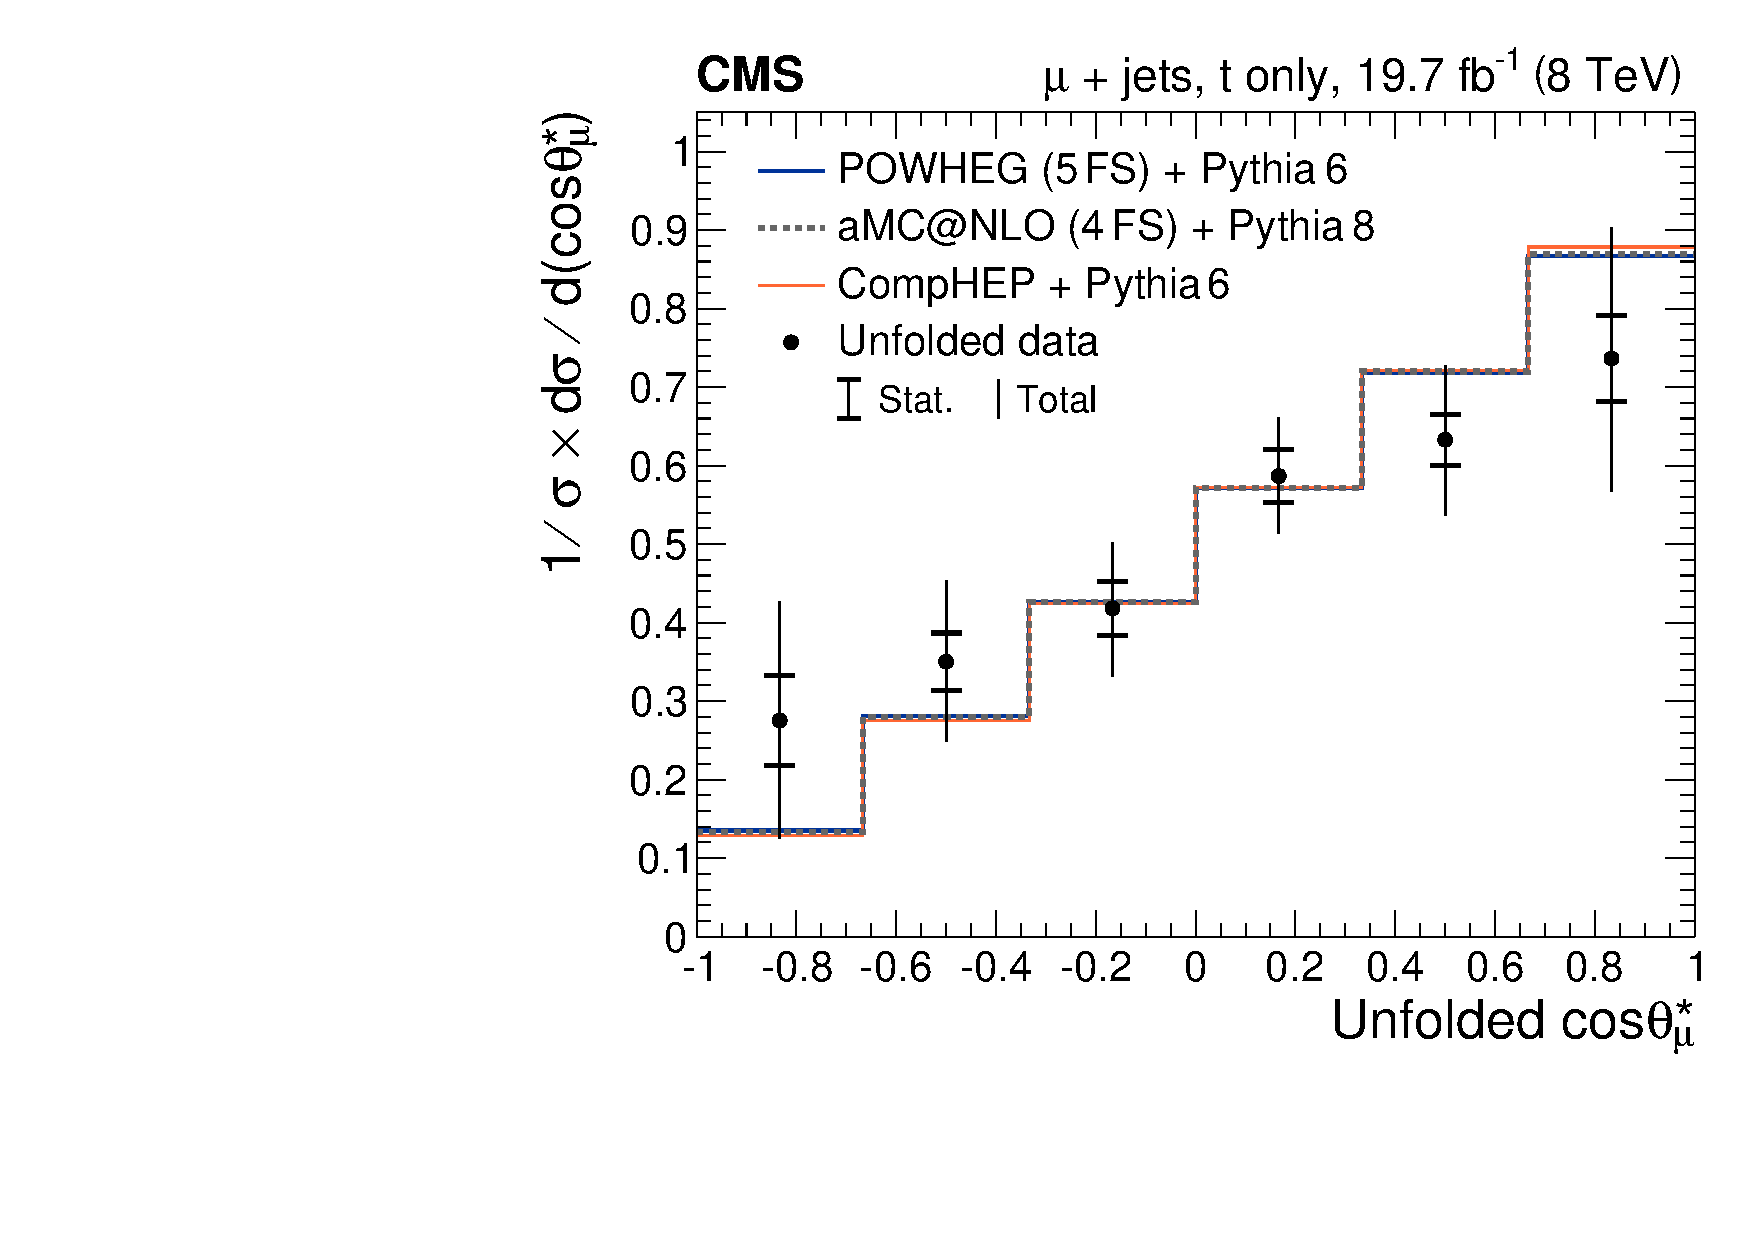
\includegraphics[width=0.48\textwidth]{figures/polarization/result/unfolded_mu_top.pdf}}
\hspace{0.02\textwidth}
\subfloat[]{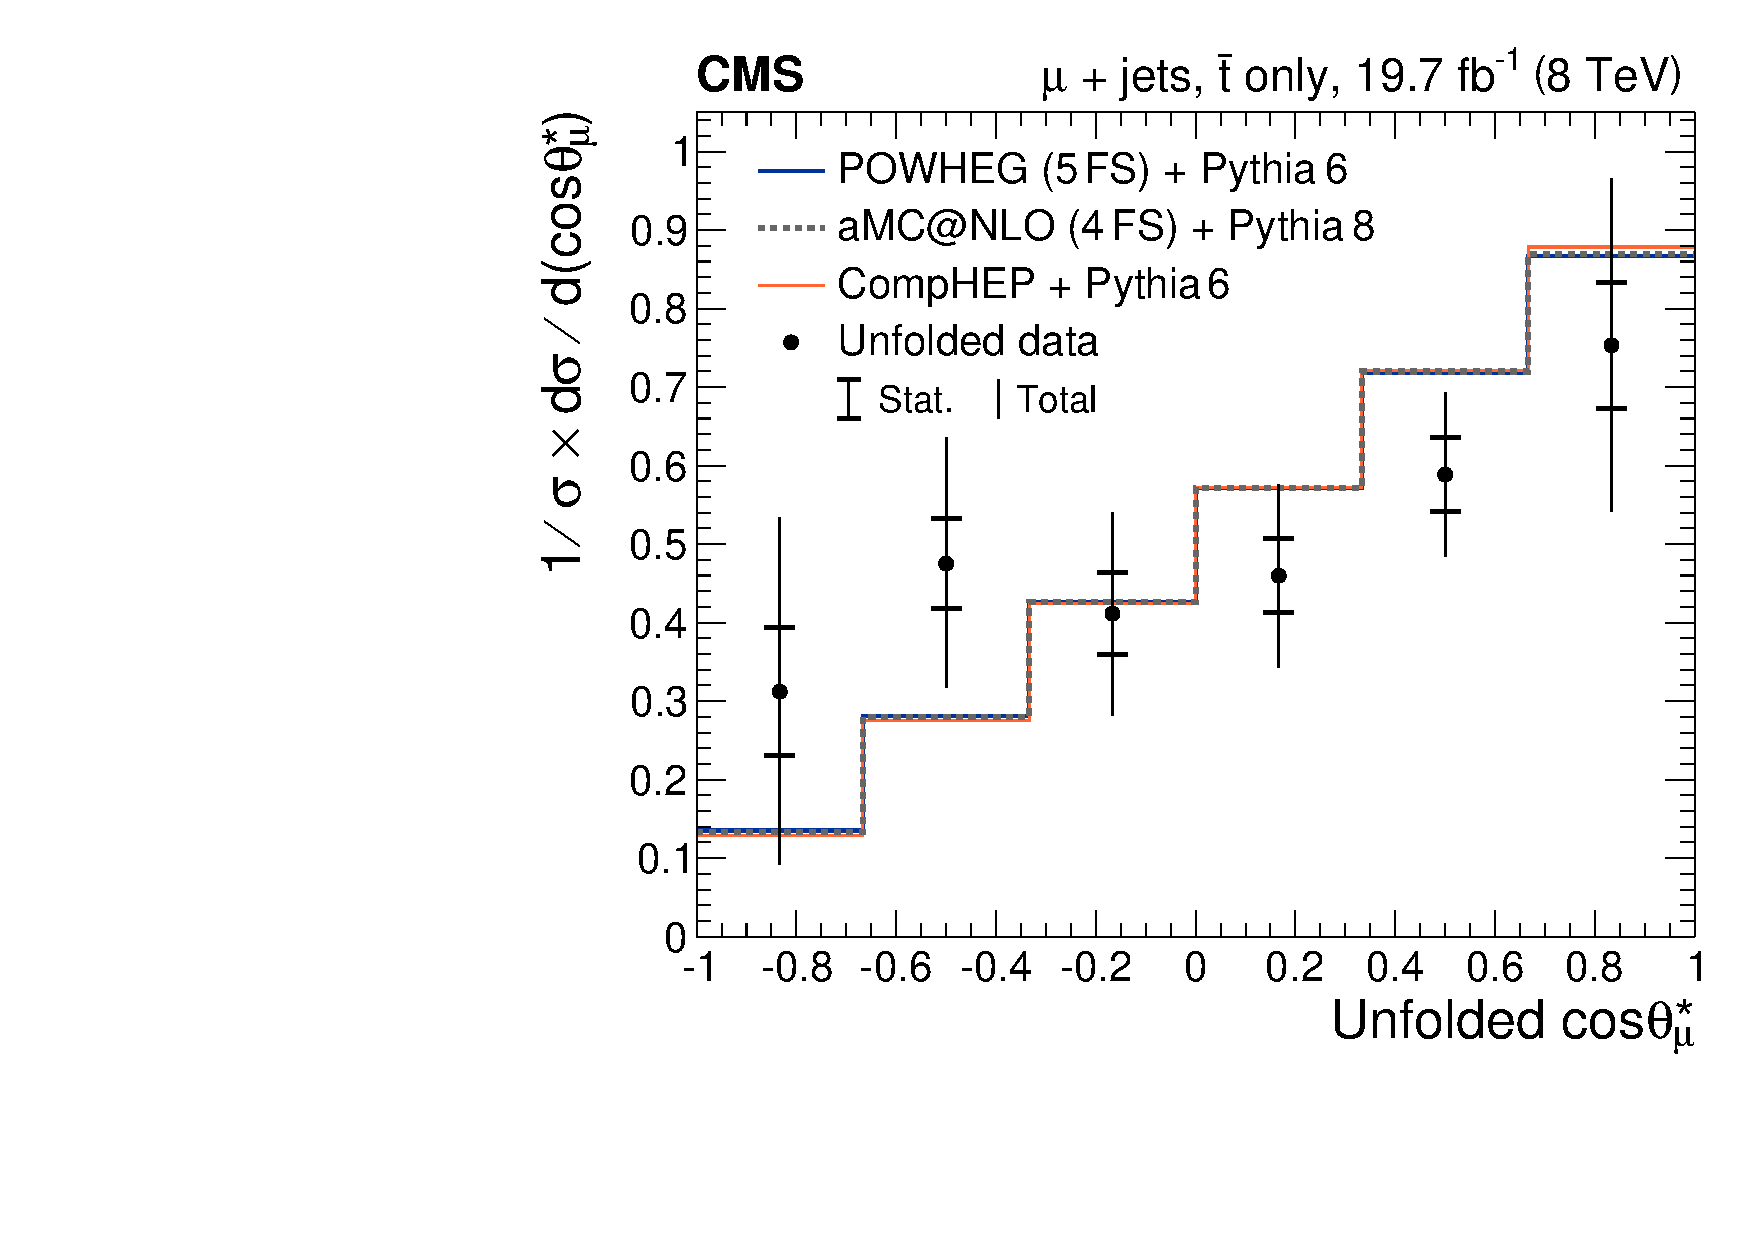
\includegraphics[width=0.48\textwidth]{figures/polarization/result/unfolded_mu_antitop.pdf}}\\
\subfloat[]{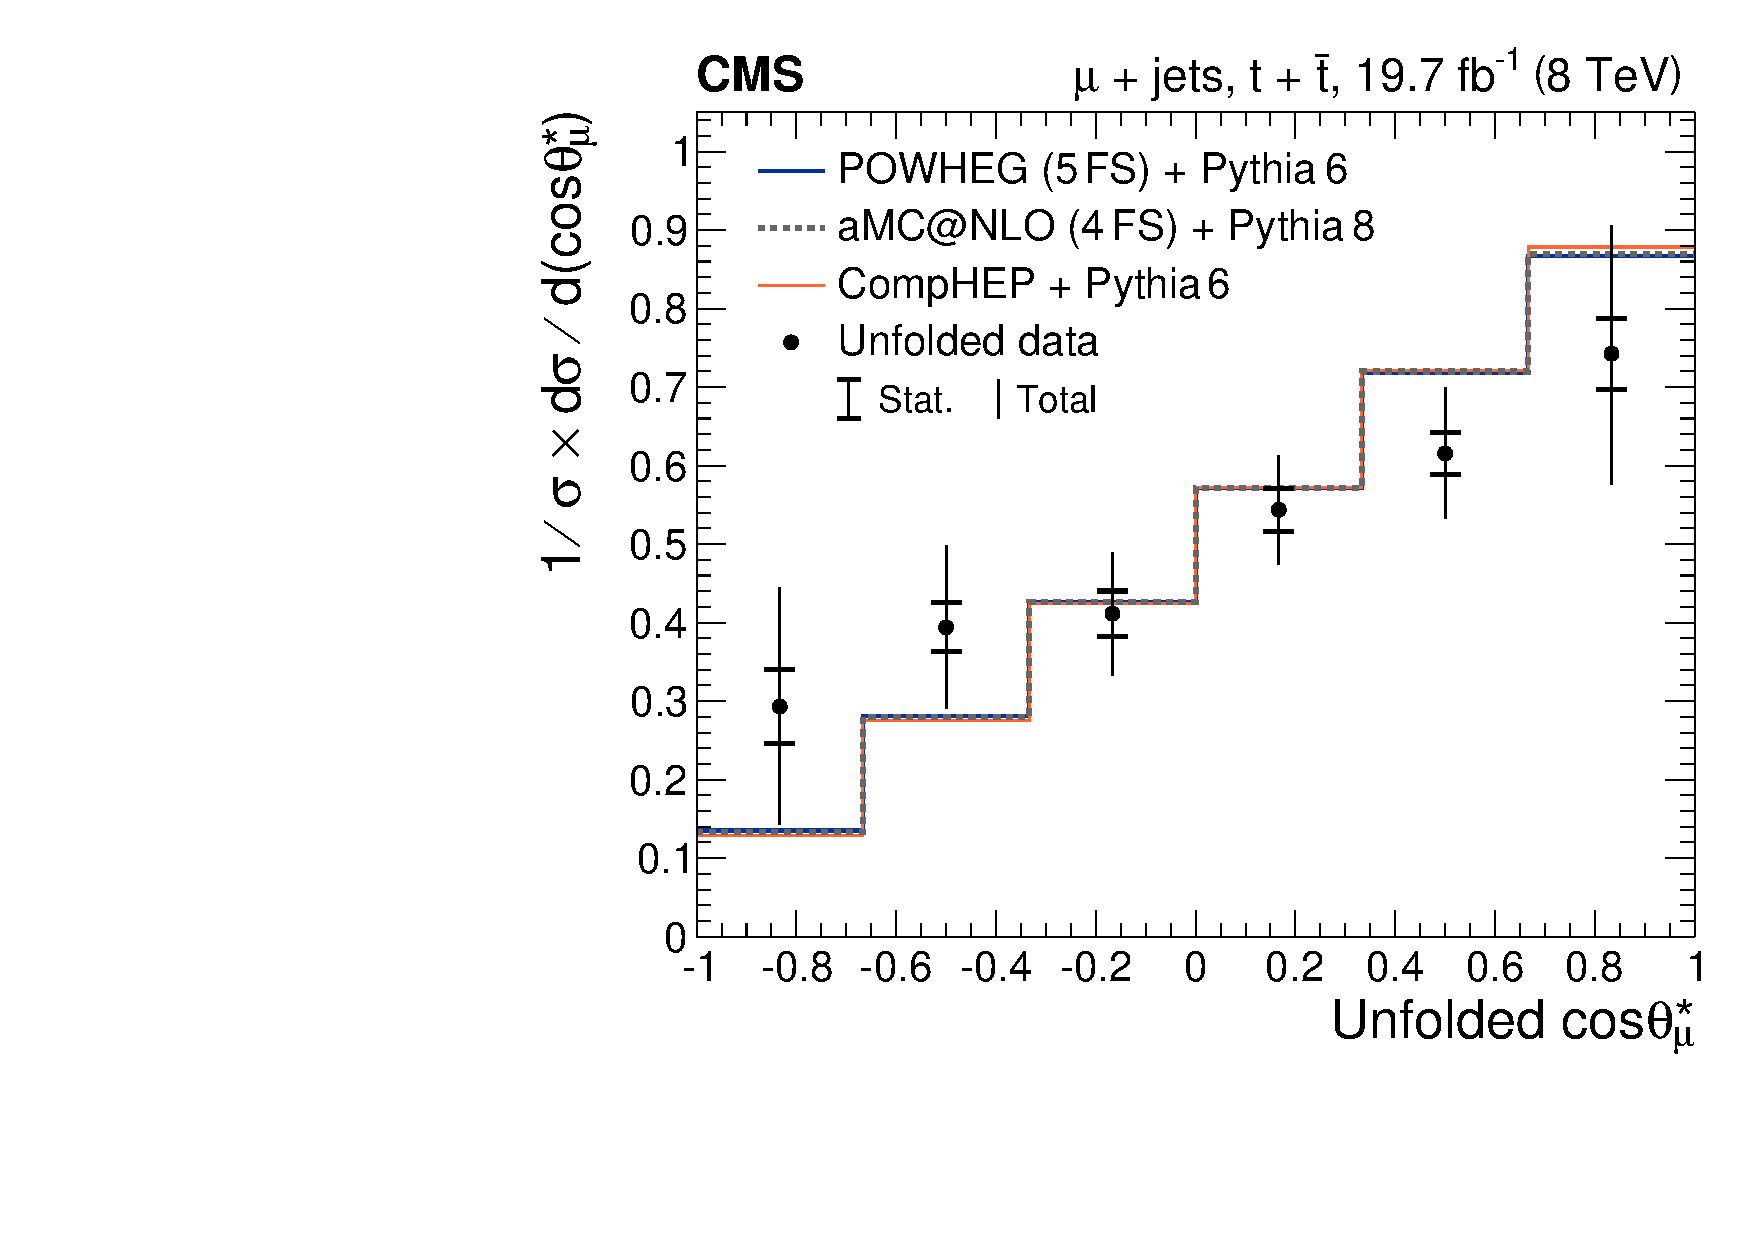
\includegraphics[width=0.48\textwidth]{figures/polarization/result/unfolded_mu.pdf}}
}


\newcommand{\AlResultCombined}{\ensuremath{\Big[26.0\pm 10.5 \Big]\cdot 10^{-2}}\xspace}
\newcommand{\AlResultCombinedStatSys}{\ensuremath{\Big[26.0\pm 2.6 \mathrm{(stat.)}\pm 10.2\mathrm{(syst.)} \Big] \cdot 10^{-2}} \xspace}
\newcommand{\AlResultCombinedPvalue}{\ensuremath{4.6\cdot 10^{-2}}\xspace}

\newcommand{\AlResultTop}{\ensuremath{\Big[29.0\pm 10.5 \Big]\cdot 10^{-2}}\xspace}
\newcommand{\AlResultTopStatSys}{\ensuremath{\Big[29.0 \pm 3.2 \mathrm{(stat.)} \pm 10.0\mathrm{(syst.)} \Big]\cdot 10^{-2}}\xspace}
\newcommand{\AlResultTopPvalue}{\ensuremath{7.9\cdot 10^{-2}}\xspace}

\newcommand{\AlResultAntiTop}{\ensuremath{\Big[21.1\pm 13.8 \Big]\cdot 10^{-2}}\xspace}
\newcommand{\AlResultAntiTopStatSys}{\ensuremath{\Big[21.1\pm 4.6\mathrm{(stat.)}\pm 12.6\mathrm{(syst.)} \Big]\cdot 10^{-2}}\xspace}
\newcommand{\AlResultAntiTopPvalue}{\ensuremath{5.0\cdot 10^{-2}}\xspace}


From data, we measure

\begin{align}
\AmuT          & = \AlResultTopStatSys = \AlResultTop , \\
\AmuTbar       & = \AlResultAntiTopStatSys = \AlResultAntiTop , \\
\AmuTplusTbar & = \AlResultCombinedStatSys = \AlResultCombined
\end{align}

using TUnfold. The measured asymmetries are compatible with a p-value of

\begin{align}
\AmuT:&\hspace{0.3cm} p(\mathrm{data |SM})          = \AlResultTopPvalue , \\
\AmuTbar:&\hspace{0.3cm} p(\mathrm{data |SM})      = \AlResultAntiTopPvalue , \\
\AmuTplusTbar:&\hspace{0.3cm} p(\mathrm{data |SM}) = \AlResultCombinedPvalue
\end{align}

with the SM value of $43.8\cdot 10^{-2}$ as predicted by \POWHEG.



\begin{align}
\AmuT          & = \Big[31.7\pm 3.7 \mathrm{(stat.)}\pm 10.9\mathrm{(syst.)} \Big]\cdot 10^{-2} = \Big[31.7\pm 11.2 \Big]\cdot 10^{-2} , \\
\AmuTbar       & = \Big[20.3\pm 5.7 \mathrm{(stat.)}\pm 15.0\mathrm{(syst.)} \Big]\cdot 10^{-2} = \Big[20.3\pm 16.0 \Big]\cdot 10^{-2} , \\
\AmuTplusTbar & = \Big[27.6\pm 3.1 \mathrm{(stat.)}\pm 11.1\mathrm{(syst.)} \Big]\cdot 10^{-2} = \Big[27.6\pm 11.5 \Big]\cdot 10^{-2} 
\end{align}

using the 2-bin analytic unfolding method as cross check.



%##############################################
\section{Limits on anomalous couplings}
%##############################################

topfit

combine: t-channel 8TeV~\cite{Khachatryan:2014iya}, Whelicity at 8TeV~\cite{Khachatryan:2016fky}


\myfigure{\label{fig:polarization-limits}Projections of limits on anomalous couplings and the top quark polarization for cases with free floating polarization~(violet) or when fixing the polarization to the anomalous couplings~(orange): (a)~left-handed vector couplings against polarization; (b)~right-handed vector coupling against polarization; (c)~left-handed tensor coupling against polarization; (d)~right-handed tensor coupling against polarization.}{
\subfloat[]{\adjincludegraphics[height=4.65cm,trim={0 0 {0.15\width} 0},clip]{figures/polarization/limits/Ptvl-nol.pdf}}
\subfloat[]{\adjincludegraphics[height=4.65cm,trim={0 0 {0.0\width} 0},clip]{figures/polarization/limits/Ptvr.pdf}}\\
\subfloat[]{\adjincludegraphics[height=4.65cm,trim={0 0 {0.15\width} 0},clip]{figures/polarization/limits/Ptgl-nol.pdf}}
\subfloat[]{\adjincludegraphics[height=4.65cm,trim={0 0 {0.0\width} 0},clip]{figures/polarization/limits/Ptgr.pdf}}
}

%\chapter{Measurement of differential single-top-quark cross sections at 13~TeV}
\label{ch:diff13}

\intro{An early measurement of the normalized differential single-top-quark cross sections in $t$~channel as a function of the top quark transverse momentum and rapidity at a \acrlong{cm} energy of 13~\TeV is presented. \Acrlong{pp} collision data corresponding to 2.3~$\mathit{fb}^\mathit{-1}$ are analyzed which were recorded in 2015 with the \gls{cms} experiment. Events containing one isolated muon and two or three jets are selected and a \acrlong{bdt} is trained for separating signal from background events further. The amount of signal events as a function of the top quark transverse momentum and rapidity is estimated by performing multiple \acrlong{ml} fits. The results are unfolded to parton level and compared to predictions by various \acrlong{mc} generators. No significant deviations are observed. The measurement detailed in this chapter has been published in Ref.~\cite{CMS-PAS-TOP-16-004} and reviewed in Ref.~\cite{Komm:2016ntr}.
}


%##############################################
\section{Outline of analysis strategy}
%##############################################

\Acrlong{pp} collision data are analyzed corresponding to an integrated luminosity of 2.3~\invfb. Events containing one isolated muon and two or three jets are selected. A \gls{bdt} is trained to obtain a powerful discriminant for separating signal from background events. The individual amounts of signal and background events in data are estimated by performing a template-based \gls{ml} fit to the distributions of the transverse W~boson mass and the \gls{bdt} discriminant in the signal and in two \ttbar-dominated control regions simultaneously. The contamination by multijet events is estimated by using a data-driven template to model its shape. The template is obtained from a sideband region for which the muon isolation is inverted. Multiple \gls{ml} fits are performed in separate intervals of the top quark transverse momentum and rapidity in addition. By passing these fit results directly to the unfolding procedure the differential cross section as a function of the top quark \pt and rapidity is inferred. The impact of sources of systematic uncertainties on the differential cross section is evaluated by repeating the measurement with correspondingly modified templates. The resulting differential cross sections are compared to predictions by various event generators.

The outlined strategy has multiple benefits compared to the one chosen for the polarization measurement~(Ch.~\ref{ch:polarization}). First, it is not necessary to define a signal-enriched region where the remaining backgrounds are subtracted from data prior to unfolding. Instead, the signal yields in intervals of the top quark \pt and rapidity are taken from the fit results directly. Secondly, since no signal-enriched region is defined an optimization of its selection is also not required. The measurement is carried out with no explicit selection to reject multijet events or on the \gls{bdt} discriminant to reject \wjets/\ttbar events except for validation purposes. Lastly, residual differences in the estimated background yields between unfolding bins are profiled per bin of the top quark \pt or rapidity spectrum. This reduces the impact of potential shortcomings in their modeling and can also mitigate a potential bias that may occur through correlations of the \gls{bdt} discriminant with the top quark \pt and rapidity distributions.



%##############################################
\section{Event selection and simulated samples}
%##############################################
\label{sec:diff13-selection}

The measurement is based on \gls{pp} collision data corresponding to 2.3~\invfb which were recorded with the \gls{cms} experiment in 2015 at a \acrlong{cm} energy of 13~\TeV. During this data taking period the instantaneous luminosity was kept relatively low with a maximum of about $5.1~\mathrm{Hz}/\mathrm{nb}$ leading to only 14~pileup interactions on average~\cite{lumipublic}. 

A muon trigger is employed which requires the presence of an isolated muon candidate with a transverse momentum of at least $20~\GeV$ within $|\eta|<2.4$. Offline, the muon candidate is required to have $\pt>22~\GeV$ within $|\eta|<2.4$ and it has to fulfill tight identification requirements as well. Furthermore, the muon candidate is required to be isolated with a relative \gls{deltabeta}-based isolation of $\muiso<6\%$, calculated from the transverse energy deposits of charged and neutral hadrons, photons, and from tracks associated to pileup interactions within a cone of $\Delta R<0.4$ around the candidate~(see Sec.~\ref{sec:reconstruction-muons}). The isolation is explicitly chosen tighter here compared to single-top-quark measurements at 8~\TeV (e.g. Ch.~\ref{ch:polarization}, Ref.~\cite{Khachatryan:2014iya}) in which an isolation of $\muiso<12\%$ is required instead. The distribution of the relative muon isolation after applying the complete event selection with the exception of the isolation requirement is presented in Fig.~\ref{fig:diff13-reliso}. The multijet template is taken exceptionally from simulation and scaled such that it fits approximately to the bulk of the data distribution within uncertainties. The deviation at high isolation values can be attributed to differences in the trigger isolation efficiencies between data and its emulation in simulation. The tighter isolation working point is motivated by the observed larger background contamination stemming from multijet production. Selection efficiencies for various working points, estimated from simulation, are listed in Tab.~\ref{tab:diff13-isoworkingpoints}. Compared to $\muiso<12\%$, the contamination by multijet events is about halved at the new working point of $\muiso<6\%$ whereas only 12\% of signal and other background events are rejected.

\myfigure{\label{fig:diff13-reliso} Distribution of the relative \gls{deltabeta}-based muon isolation in 2j1t. The multijet template is taken from simulation.}{
\subfloat[]{\adjincludegraphics[height=4.8cm,trim={0 0 {0.\width} 0},clip]{figures/differential/plots/2j1t/2j1t_relIso_qcdnone.pdf}}
}

\mytable{\label{tab:diff13-isoworkingpoints}Selection efficiencies for various isolation working points estimated from simulation.}{
\begin{tabular}{@{}l c c c c@{}}
\toprule
Process \hspace{1.7cm}        & \multicolumn{4}{c}{Selection efficiency} \\
\cmidrule{2-5}
& \hspace{0.2cm}$\muiso<12\%$\hspace{0.2cm}
& \hspace{0.2cm}$\muiso<8\%$\hspace{0.2cm}
& \hspace{0.2cm}$\muiso<6\%$\hspace{0.4cm}
& $\muiso<4\%$ \\
\midrule
$t$~channel       & 94\% & 88\% & 83\% & 73\% \\
Multijet (simulation) & 33\% & 21\% & 16\% & 10\% \\
Other backgrounds & 93\% & 87\% & 82\% & 72\% \\
\bottomrule     

\end{tabular}
}

For the measurement, contributions from processes with a $\mu\mu\mathrm{\mbox{+}jets}$ or a $\mu\mathrm{e}\mathrm{\mbox{+}jets}$ final state such as dileptonic \ttbar or \zjets production are suppressed by vetoing events containing additional muon~($\pt>10~\GeV$, $|\eta|<2.5$) or electron candidates~($\pt>20~\GeV$, $|\eta|<2.5$). Additional muon candidates are required to be isolated~($\muiso<20\%$) and to fulfill loose identification criteria. Electrons candidates on the other hand have to pass identification criteria which are specifically designed for vetoing events containing additional electrons.

Jets are clustered from \Gls{pf} candidates using the anti-\kt algorithm with a distance parameter of $R=0.4$ while mitigating the influence of pileup through the \gls{chs} technique~\cite{CMS-PAS-JME-14-001}. The reconstructed jet energy is corrected in data and simulation using dedicated scale factors. Additionally, the jet energy is smeared in simulation to match the resolution observed in data. Events containing two or three jets with a corrected transverse momentum of at least $40~\GeV$ that fall within $|\eta|<4.7$ and fulfill loose identification requirements are selected for analysis. Potential overlaps between selected jets and the single muon candidate are avoided by ignoring jets that are reconstructed within a cone of $\Delta R<0.3$ around the muon. The \gls{csv} algorithm (version~2) is employed for b-tagging~\cite{CMS-PAS-BTV-15-001}. At its tight working point an efficiency of about 50\% is achieved for tagging true b~jets whereas the fraction of mistagged jets originating from g, u, d, s quarks amounts to only 0.1\%. To match the observed b-tagging efficiency in data, simulated events are reweighted using dedicated scale factors.

For validation purposes, events with a transverse W~boson mass of $\mtw>50~\GeV$ are selected to reject multijet events. However, the region $\mtw<50~\GeV$ is explicitly kept in the measurement since it provides sensitivity to estimate the amount of multijet events as detailed in Sec.~\ref{sec:diff13-fit}.

The following samples of simulated events are employed in the measurement. The \MGAMC generator interfaced with \PYTHIA{}\,8 is used to generate the default signal sample of $t$-channel single-top-quark production in 4~\gls{fs}. Alternative samples are generated for comparison using the \MGAMC generator interfaced with \PYTHIA{}\,8 in 5~\gls{fs}, \MGAMC interfaced with \HERWIG in 4~\gls{fs}, and \POWHEG interfaced with \PYTHIA in 4~\gls{fs}. Single-top-quark production via tW and \ttbar production are simulated using the \POWHEG generator interfaced with \PYTHIA{}\,8. Samples of \wjets and \zjets events are generated using \MGAMC interfaced with \PYTHIA{}\,8 as well. The calculated \gls{sm} cross sections for normalizing these samples are listed in Tab.~\ref{tab:diff13-theo-xsecs}. The contributions by single-top-quark production in $s$~channel and by diboson production have been found negligible at 13~\TeV after the event selection. Thus corresponding samples are not used in the measurement. Special care is taken for normalizing the samples produced with the \MGAMC generator because the \gls{mcatnlo} matching scheme leads to a significant fraction of negatively weighted events. In the employed samples the fractions are found to be about 40\% for $t$-channel, 25\% for \zjets, and 15\% for \wjets events.

\mytable{\label{tab:diff13-theo-xsecs}Theoretical \gls{sm} cross sections at 13~TeV used to normalize the simulated samples.}{
\begin{tabular}{@{}l  r c l@{}}
\toprule
Process & \hspace{0.5cm}Cross section & & Accuracy \\
\midrule
$t$-channel top quark & $136.0^{+5.4}_{-4.6}~\pb$ && \gls{nlo} \hfill (using \HATHOR\,2.1~\cite{Aliev:2010zk})   \\
$t$-channel top antiquark & $81.0^{+4.1}_{-3.6}~\pb$ && \gls{nlo} \hfill (using \HATHOR\, 2.1~\cite{Aliev:2010zk})   \\
tW~channel & $71.7\pm3.8~\pb$ && \gls{nlo} \hfill (using \HATHOR\,2.1~\cite{Aliev:2010zk})  \\
\ttbar & $832^{+20}_{-29}~\pb$ && \gls{nnlo} \hfill (using \TOPPP\,2.0~\cite{Czakon:2011xx}) \\
$\mathrm{W}\to\ell\nu\mathrm{\,\mbox{+}\,jets}$ & $20\,509^{+788}_{-776}~\pb$ && \gls{nnlo} \hfill (using \FEWZ\,3.1~\cite{Li:2012wna}) \\
$\mathrm{Z}/\gamma^{*}\to\ell^{\rmplus}\ell^{\rmminus}$, $m_{\ell\ell}>50~\GeV$ & $2\,008^{+76}_{-75}~\pb$ && \gls{nnlo} \hfill (using \FEWZ\,3.1~\cite{Li:2012wna}) \\
\bottomrule
\end{tabular}
}

Following a similar procedure as in the top quark polarization measurement~(Ch.~\ref{ch:polarization}), the shape of multijet events is modeled by a data-driven template from a sideband region for which the muon isolation is inverted as $\muiso>20\%$ in the event selection. A systematic uncertainty on the shape of the multijet template is taken into account by extracting the template from an isolation subrange of either $\muiso\in[20\%,40\%]$ or $\muiso\in[40\%,\infty]$ instead. These intervals have been chosen such that they contain approximately equal amounts of data events in order not to increase the . The resulting shape variations after scaling each template to its individual \gls{ml} fit result are shown in Fig.~\ref{fig:diff13-qcd-sys-mtw} as a function of the transverse W~boson mass. In Fig.~\ref{fig:diff13-qcd-sys-bdt} the shape uncertainty as a function of a \gls{bdt} discriminant~(Sec.~\ref{sec:diff13-bdt}) is shown in a multijet-depleted region defined by $\mtw>50~\GeV$. In this region the uncertainty on the extrapolated multijet yield amounts to about $\pm20\%$ on average. In the distributions throughout this chapter, the extracted multijet template as well as other background and signal templates are scaled to the result of a \gls{ml} fit to data as described in Sec.~\ref{sec:diff13-fit} unless explicitly stated otherwise.

\myfigure{\label{fig:diff13-qcd-sys}Extracted multijet templates from three sideband regions with different muon isolation ranges in 2j1t region: (a)~distribution of the transverse W~boson mass; (b)~distribution of a \gls{bdt} discriminant for events with $\mtw>50~\GeV$. The individual templates are scaled to the results of corresponding \gls{ml} fits to data~(Sec.~\ref{sec:diff13-fit}).}{
\subfloat[\label{fig:diff13-qcd-sys-mtw}]{\adjincludegraphics[height=4.8cm,trim={0 0 {0.18\width} 0},clip]{figures/differential/qcdshapes/reco_mtw_QCD_2j1t__Iso_nol.pdf}}
\subfloat[\label{fig:diff13-qcd-sys-bdt}]{\adjincludegraphics[height=4.8cm,trim={0 0 {0.\width} 0},clip]{figures/differential/qcdshapes/reco_BDT_QCD_2j1t__Iso.pdf}}
}


After the event selection signal and control regions are defined based on the number of selected jets and the subset of jets which are also b-tagged. The same notation as in the top quark polarization measurement is employed as detailed in Sec.~\ref{sec:polarization-selection}. In control regions the assignment of jets to the top quark decay and to the spectator quark is performed as follows. First, b-tagged jets are sorted by \pt and non-tagged jets by $|\eta|$. Then, the most forward jet is taken as the spectator jets because in $t$-channel single-top-quark production it is expected to be scattered into the forward detector region by recoiling against the W~boson. In the 2j0t control region the remaining jet is then associated to the top quark decay. In control regions containing multiple b-tagged jets the top quark is reconstructed using the hardest b-tagged jet. This choice is motivated by the fact that an additional b~quark in $t$-channel single-top-quark production originates from initial state gluon splitting for which a softer spectrum is expected.

Distributions of the reconstructed top quark mass in signal and control regions are presented in Fig.~\ref{fig:diff13-topmass}. Since the 3j2t region contains a relatively low number of events, the 3j1t region is considered as an additional \ttbar control region in this analysis for fitting. The shown distributions of data are well described by the simulated signal and background samples, and the extracted multijet templates.

 
\myfigure{\label{fig:diff13-topmass} Distributions of the reconstructed top quark mass: (a)~\wjets control region; (b)~signal region; (c+d)~\ttbar control regions.}{
\subfloat[]{\adjincludegraphics[height=4.8cm,trim={0 0 {0.16\width} 0},clip]{figures/differential/plots/2j0t/2j0t_top_mass_qcdnone_nol.pdf}}
\subfloat[]{\adjincludegraphics[height=4.8cm,trim={0 0 {0.\width} 0},clip]{figures/differential/plots/2j1t/2j1t_top_mass_qcdnone.pdf}}\\
\subfloat[]{\adjincludegraphics[height=4.8cm,trim={0 0 {0.16\width} 0},clip]{figures/differential/plots/3j1t/3j1t_top_mass_qcdnone_nol.pdf}}
\subfloat[]{\adjincludegraphics[height=4.8cm,trim={0 0 {0.\width} 0},clip]{figures/differential/plots/3j2t/3j2t_top_mass_qcdnone.pdf}}
}


%##############################################
\section{Background modeling}
%##############################################
\label{sec:diff13-modeling}

The modeling of the simulated samples and the applied corrections are assessed. In Fig.~\ref{fig:diff13-njet-validation} distributions of the number of jets and the number of b-tagged jets are presented. These allow to validate whether if the applied jet energy corrections and the b-tagging efficiency scale factors correct properly for any residual differences between data and simulation. Good agreement is observed for the number of b-tagged jets and also for the number of jets at low multiplicities~($N\leq4$) relevant for this analysis. At higher jet multiplicities, the number of jets is overestimated by simulation to which the measurement is however not sensitive. Dedicated \ttbar measurements revealed that a refining of generator parameters controlling the radiation of addition partons results in a good description of data at high jet multiplicities as well~\cite{CMS-PAS-TOP-16-021}.

\myfigure{\label{fig:diff13-njet-validation} Distributions of the number of selected jets and b-tagged jets for events with at least two selected jets and $\mtw>50~\GeV$.}{
\subfloat[]{\adjincludegraphics[height=4.8cm,trim={0 0 {0.16\width} 0},clip]{figures/differential/plots/Xj/Xj_njets_qcdmtw_nol.pdf}}
\subfloat[]{\adjincludegraphics[height=4.8cm,trim={0 0 {0.\width} 0},clip]{figures/differential/plots/Xj/Xj_nbjets_qcdmtw.pdf}}
}

The modeling of the data-driven multijet template is validated in Fig.~\ref{fig:diff13-2j0t-qcd-validation} where the distributions of the missing transverse energy and the difference in $\phi$ angles between the muon and the transverse momentum is presented in the 2j0t \wjets and 2j1t signal regions. Both distributions demonstrate a good description of data by the multijet templates and the simulated samples.

\myfigure{\label{fig:diff13-2j0t-qcd-validation} Validation of the data-driven multijet template in (top row)~2j0t \wjets control region and (bottom row)~2j1t signal region: (left column)~distribution of the missing transverse energy; (right column)~distribution of the difference of the $\phi$ angles of the muon and missing transverse momentum.}{
\subfloat[]{\adjincludegraphics[height=4.8cm,trim={0 0 {0.16\width} 0},clip]{figures/differential/plots/2j0t/2j0t_met_qcdnone_nol.pdf}}
\subfloat[]{\adjincludegraphics[height=4.8cm,trim={0 0 {0.\width} 0},clip]{figures/differential/plots/2j0t/2j0t_muon_met_deltaPhi_qcdnone.pdf}}\\
\subfloat[]{\adjincludegraphics[height=4.8cm,trim={0 0 {0.16\width} 0},clip]{figures/differential/plots/2j1t/2j1t_met_qcdnone_nol.pdf}}
\subfloat[]{\adjincludegraphics[height=4.8cm,trim={0 0 {0.\width} 0},clip]{figures/differential/plots/2j1t/2j1t_muon_met_deltaPhi_qcdnone.pdf}}
}

Lastly, the \wjets modeling is assessed. Figure~\ref{fig:diff13-2j0t-wjet-validation} shows the distributions of the transverse W~boson mass and the polarization angle using the default \wjets sample generated with \MGAMC at \gls{nlo}. For comparison, the predicted shape by an alternative \wjets sample generated \MG at \gls{lo} is also presented. The sample produced with the new \MGAMC generator displays a superior modeling of both observables whereas the \MG \wjets sample exhibits some mismodeling. The trend in the ratios is somewhat different here compared to the observations in the top quark polarization measurement at 8~\TeV~(Sec.~\ref{sec:polarization-modeling}). This may be related to differences in the \PYTHIA tunes\footnote{8~\TeV: \PYTHIA{}6 $\mathrm{Z2}^\star$ tune~\cite{Chatrchyan:2011id}; 13~\TeV: \PYTHIA{}8 CUETP8M1 tune~\cite{Khachatryan:2015pea}.} which was however not studied further.

\myfigure{\label{fig:diff13-2j0t-wjet-validation} \wjets modeling in 2j0t control region by (top row)~\MGAMC at \gls{nlo} or by (bottom row)~\MG at \gls{lo} accuracy: (left column)~distribution of the \pt of the reconstructed W~boson candidate; (right column)~distribution of the polarization angle.}{
\subfloat[]{\adjincludegraphics[height=4.8cm,trim={0 0 {0.16\width} 0},clip]{figures/differential/plots/2j0t/2j0t_wboson_pt_qcdmtw_nol.pdf}}
\subfloat[]{\adjincludegraphics[height=4.8cm,trim={0 0 {0.\width} 0},clip]{figures/differential/plots/2j0t/2j0t_cosTheta_tPL_qcdmtw.pdf}}\\
\subfloat[]{\adjincludegraphics[height=4.8cm,trim={0 0 {0.16\width} 0},clip]{figures/differential/plots/2j0t/2j0t_wboson_pt_qcdmtw_MG_nol.pdf}}
\subfloat[]{\adjincludegraphics[height=4.8cm,trim={0 0 {0.\width} 0},clip]{figures/differential/plots/2j0t/2j0t_cosTheta_tPL_qcdmtw_MG.pdf}}
}


\clearpage
%##############################################
\section{BDT training}
%##############################################
\label{sec:diff13-bdt}

A \bdt is trained for separating $t$-channel single-top-quark events from \wjets and \ttbar background events. It is configured as follows. The \ADABOOST algorithm with a learning rate of 40\% is chosen. In total, 1\,000 decision trees with a maximum depth of three are trained. The number of tested working points per observables is set to 40. Negatively weighted events generated by \MGAMC are also included in the training for which the boosting weight is automatically inverted inside \TMVA. A potential overtraining through the large fraction of negatively weighted events is mitigated by adding alternative $t$-channel and \wjets events generated with \POWHEG and \MG to the training respectively whose events weights are all positive. For validation purposes an alternative \gls{bdt} is trained as well using the \GRADIENTBOOST algorithm with a shrinkage of 40\% while keeping the other settings identical. In the case significant differences in the performances between both \glspl{bdt} are obtained, this may reveal potential problems with the chosen setup hinting to e.g. overtraining or improper handling of the negatively weighted events.

In addition to the \wjets and \ttbar events a sample of simulated multijet events is added to the training as background as well. The motivation for this is to prevent that multijet events become accidentally clustered at high values of the final \gls{bdt} discriminant. The exact amount of mixed-in multijet events has to be however carefully chosen since if it is too large the \gls{bdt} might separate multijet from signal events predominantly while mostly ignoring \wjets and \ttbar events.

Various input observables have been investigated for their individual discrimination power per process-pair as listed in Tab.~\ref{tab:diff13-aucs}. The following five observables have been chosen which provide individually already a high discrimination power while exhibiting low correlations with the reconstructed top quark \pt and rapidity:

\begin{itemize}
\item the absolute value of the pseudorapidity of the untagged spectator jet~(\jprime);
\item the invariant mass of the reconstructed top quark candidate;
\item the $\Delta R$ distance between the two selected jets;
\item the difference in pseudorapidity between the muon and the selected b-tagged jet;
\item the transverse W~boson mass, \mtw, before solving for the unknown neutrino $p_{z}$ component in the top quark reconstruction.
\end{itemize} 

\mytable{\label{tab:diff13-aucs}Discrimination power of event observables and the trained \glspl{bdt} in 2j1t region for various combinations of signal ($t$-channel) and background (\ttbar, \wjets, multijet) processes. Highlighted are a few of the most discriminating observables per process-pair.}{
\begin{tabular}{@{}l l rr rr rr rr@{}}
\toprule
\hspace{0.3cm} & Observable  &  \multicolumn{8}{c }{Area under \gls{roc} curve (\gls{auc})} \\
\cmidrule{3-10}
&  & \multicolumn{2}{c}{\ttbar/signal\hspace{0.1cm}} & \multicolumn{2}{c}{\hspace{0.1cm}\wjets/signal\hspace{0.2cm}} & \multicolumn{2}{c}{\hspace{0.1cm}Multijet/signal\hspace{0.2cm}} & \multicolumn{2}{c@{}}{\hspace{0.1cm}\ttbar/\wjets}  \\
\midrule
\multirow{5}{*}{\rotatebox[origin=c]{90}{\gls{bdt} inputs}} 
& Spectator jet $|\eta(\jprime)|$                        &\hspace{0.4cm} \textbf{26\%}&   &\hspace{0.6cm} 21\%&   & \hspace{0.7cm}10\%& &\hspace{0.7cm} 6\%& \\
& $|m_\mathrm{top}-172.5~\GeV|$                 & 13\%&   & \textbf{24\%}&   & 14\%& & 11\%& \\
& $\Delta R(\mathrm{b~jet},\,\jprime)$          & \textbf{26\%}&   & 13\%&   & 5\%& & \textbf{15\%}& \\
& $|\Delta\eta(\mathrm{b~jet},\,\mathrm{muon})|$& 5\%&   & \textbf{20\%}&   & 5\%& & \textbf{16\%}& \\
& \mtw                                          & 4\%&   & 2\%&   & \textbf{36\%}& & 3\%& \\
\midrule 
\multirow{11}{*}{\rotatebox[origin=c]{90}{Others}} 
& \met                                          & 9\%&   & 4\%&   & \textbf{28\%}& & 12\%& \\
& Muon \pt                                      & 11\%&   & 10\%&   & \textbf{27\%}& & 1\%& \\
& Spectator jet \pt                             & 1\%&   & 4\%&   & 9\%& & 4\%& \\
& $|\Delta\phi(\mathrm{muon},\,\met)|$          & 6\%&   & 3\%&   & 19\%& & 4\%& \\
& b~jet mass                                    & 5\%&   & 3\%&   & 8\%& & 5\%& \\
& Dijet \pt                                     & 12\%&   & 4\%&   & 6\%& & 8\%& \\
& Dijet mass                                    & 23\%&   & 14\%&   & 11\%& & 10\%& \\
& $\sqrt{\hat{s}}=|\vec{p}_\mathrm{top}+\vec{p}_{\jprime}|$                                     
                                                & 15\%&   & 7\%&   & 11\%& & 8\%& \\
& $(\vec{p}_\mathrm{top}+\vec{p}_{\jprime})_\mathrm{T}$                                 
                                                & 16\%&   & 1\%&   & 1\%& & \textbf{17\%}& \\
& Isotropy                                      & 2\%&   & 4\%&   & 8\%& & 6\%& \\
& Sphericity                                    & \textbf{25\%}&   & 18\%&   & 7\%& & 10\%& \\
& Event shape C                                 & \textbf{25\%}&   & 17\%&   & 7\%& & 10\%& \\
& $\cos\theta^\star_\mu$ (polarization)         & 14\%& & 7\%& &9\%& &7\%&\\
& $\cos\theta^\star_\mathrm{W}$ (helicity)      & 1\%& & 11\%& &10\%& &10\%&\\
 \midrule
& \gls{bdt} (\ADABOOST)                         & 31\%&   & 32\%&   & 27\%& & 3\%& \\
& \gls{bdt} (\GRADIENTBOOST)                    & 31\%&   & 31\%&   & 29\%& & 2\%& \\
\bottomrule
\end{tabular}
}

Although \mtw provides little discrimination power for separating $t$-channel from \wjets and \ttbar events it is included for its discrimination power against multijet events. The event shape variables C and sphericity yield a high discrimination power as well for separating signal from \ttbar events as indicated in Tab.~\ref{tab:diff13-aucs}. They are calculated as

\begin{equation}
S^{ab}=\frac{\mathlarger{\sum}\limits_{i}^{\mathrm{jets},\,\mu,\,\pvmiss}\,p_{i}^{a}\cdot p_{i}^{b}}{\mathlarger{\sum}\limits_{i}^{\mathrm{jets},\,\mu,\,\pvmiss}\,|\vec{p}_{i}|^2}\,,\quad \Rightarrow~S=\frac{3}{2}(\lambda_2+\lambda_3)\,,\quad C=3(\lambda_1\lambda_2+\lambda_1\lambda_3+\lambda_2\lambda_3)\,,
\end{equation}

where $\lambda_1+\lambda_2+\lambda_3=1$ are the decreasingly-ordered eigenvalues of the momentum tensor $S^{ab}$. Their distributions are shown in Fig.~\ref{fig:diff13-eventshapes} for which also a good modeling of data by the simulated samples is observed. However, when adding these observables to the \gls{bdt} training no further improvement in discrimination power was obtained. Thus they have been omitted from the \gls{bdt} training for the measurement.

\myfigure{\label{fig:diff13-eventshapes}Event shape observables in 2j1t region: (a)~event shape C; (b)~sphericity. Details on their calculation are given in the text.}{
\subfloat[]{\adjincludegraphics[height=4.8cm,trim={0 0 {0.16\width} 0},clip]{figures/differential/plots/2j1t/2j1t_C_qcdmtw_nol.pdf}}
\subfloat[]{\adjincludegraphics[height=4.8cm,trim={0 0 {0.\width} 0},clip]{figures/differential/plots/2j1t/2j1t_sphericity_qcdmtw.pdf}}
}

The trained \gls{bdt} discriminant yields an \gls{auc} of 31\% and 32\% for separating $t$-channel single-top-quark events from \ttbar and \wjets events, respectively. The obtained performance is confirmed by the alternative \gls{bdt} which is trained with the \GRADIENTBOOST method instead. The \gls{bdt} discrimination power against multijet events of $27\%$ is not as high as what could be obtained with the transverse W~boson mass alone ($36\%$). This is a result of the reduced amount of multijet events added to the training such that the \gls{bdt} does not discriminates against them predominantly but mostly against \ttbar and \wjets events instead.

Distributions of the chosen input observables in the 2j1t region are shown in Fig.~\ref{fig:diff13-training-obs} which the exception of the top quark mass which has already been presented in Fig.~\ref{fig:diff13-topmass}. The distribution of the resulting \gls{bdt} discriminant is shown in Fig.~\ref{fig:diff13-bdt-raw}. Since its shape is used later in an \gls{ml} fit an ad-hoc transformation 

\begin{equation}
\bdt\mapsto\bdt^\prime=\tanh\Big(3.2\cdot\big(\bdt-0.12\big)\Big)
\end{equation}

is applied to the \gls{bdt} value per event such that the distribution has an improved spread over the full range of $\bdt\in[-1;1]$ for fitting. The exact transformation is chosen such that multiple bins with varying signal fractions are obtained which yields a higher sensitivity to the signal yield in the fit.

\myfigure[p]{\label{fig:diff13-training-obs} Distributions of some input observables for the \gls{bdt} training in 2j1t signal region and the final discriminant: (a)~the transverse W~boson mass; (b)~pseudorapidity of the spectator jet~(\jprime); (c)~$\Delta R$ difference between the two jets; (d)~difference in pseudorapidities between the muon and b-tagged jet; (e+f)~the raw and transformed discriminant. The hatched band reflects the total systematic uncertainties. The figures are taken from Ref.~\cite{CMS-PAS-TOP-16-004}.}{
\subfloat[]{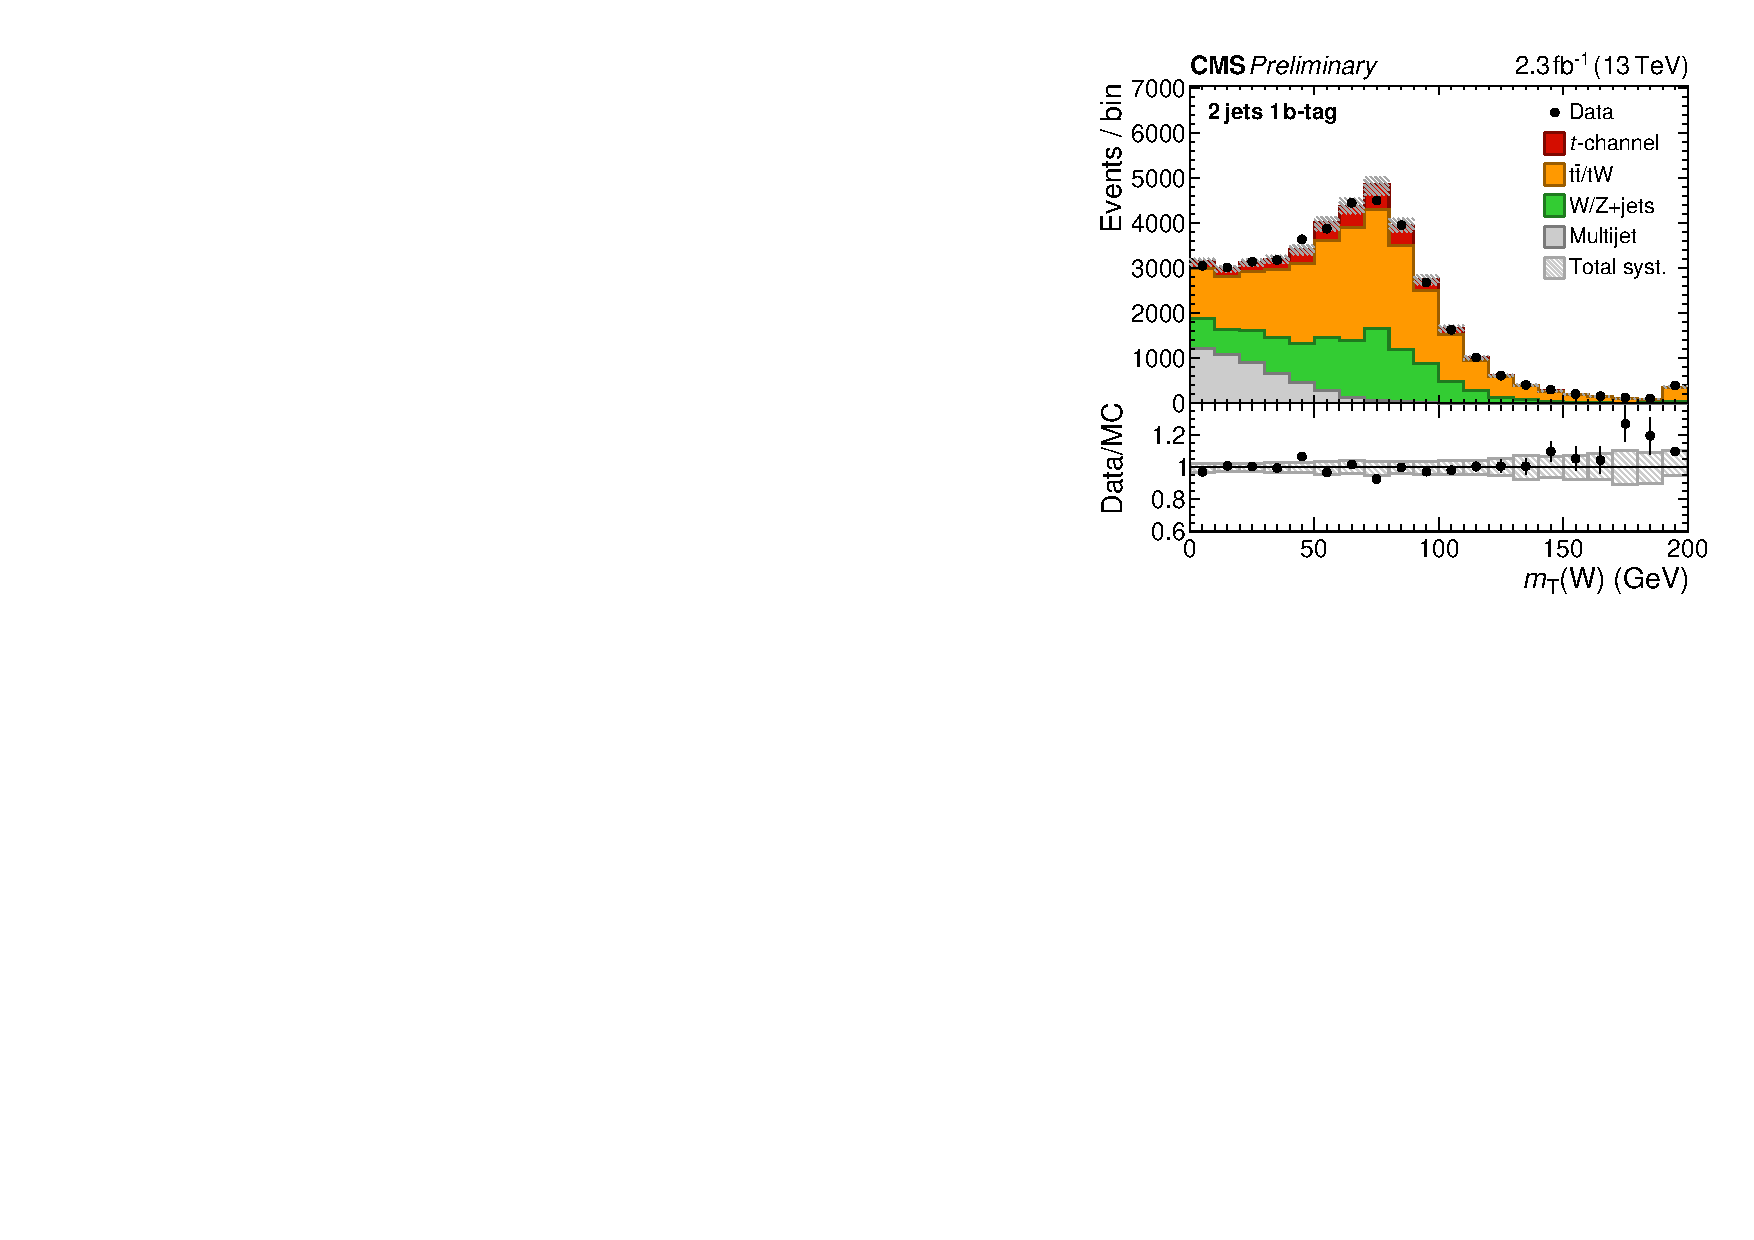
\includegraphics[width=0.48\textwidth]{figures/differential/pas/reco_mtw.pdf}}
\hspace{0.02\textwidth}
\subfloat[\label{fig:diff13-training-obs-etaj}]{\includegraphics[width=0.48\textwidth]{figures/differential/pas/reco_etaj.pdf}}\\
\subfloat[]{\includegraphics[width=0.48\textwidth]{figures/differential/pas/reco_dR.pdf}}
\hspace{0.02\textwidth}
\subfloat[]{\includegraphics[width=0.48\textwidth]{figures/differential/pas/reco_dEta.pdf}}\\
\subfloat[\label{fig:diff13-bdt-raw}]{\includegraphics[width=0.48\textwidth]{figures/differential/pas/reco_BDT_unw.pdf}}
\hspace{0.02\textwidth}
\subfloat[\label{fig:diff13-bdt-mod}]{\includegraphics[width=0.48\textwidth]{figures/differential/pas/reco_BDT.pdf}}
}

The correlations between the top quark \pt, rapidity, and the \gls{bdt} input observables for $t$-channel single-top-quark events are presented in Fig.~\ref{fig:diff13-correlation-inputs}. In general, the correlations with the top quark \pt and rapidity are found to be relatively low. For the top quark rapidity the largest correlation amounts to $8\%$ with the transverse W~boson mass while for the top quark \pt a correlation of $-14\%$ is observed with the pseudorapidity of the spectator jet.

\myfigure{\label{fig:diff13-correlation-inputs}Pearson correlation coefficients between the \gls{bdt} input observables and the top quark \pt and rapidity for $t$-channel single-top-quark events.}{
\includegraphics[width=0.8\textwidth]{figures/differential/ObsCorrelations.pdf}
}


%##############################################
\section{Signal extraction}
%##############################################
\label{sec:diff13-fit}

In past single-top-quark measurements (e.g. Refs.~\cite{Khachatryan:2015dzz,Khachatryan:2014iya,Sirunyan:2016cdg}), the contamination by multijet events is estimated following a common procedure in which an extra \gls{ml} fit to data is performed using the \mtw or \met distribution while keeping all other processes grouped together. The amount of signal events is then estimated by performing a second \gls{ml} fit using a discriminating observables such as the pseudorapidity of the spectator jet or an \gls{mva} discriminant while fixing the multijet yield to the first fit result. The reason behind this two-staged fitting procedure is that the \mtw or \met shape is very sensitive to the multijet yield whereas another observable is required to provide sufficient sensitivity to break down the contributions by the signal and the other background processes~(see also Tab.~\ref{tab:diff13-aucs}). In this measurement a novel fitting strategy, outlined in the following, has been developed which allows to simultaneously estimated the amount of signal, the contamination by multijet events, and the contributions by the other backgrounds processes by performing only a single \gls{ml} fit. The log-likelihood of the fit can be written as

\begin{equation}
\ln\big(\mathsf{L}_\mathrm{total}\big)=\ln\big(\mathsf{L}^\mathrm{2j1t}_\mathrm{Poi.}\big)+\ln\big(\mathsf{L}_\mathrm{Poi.}^\mathrm{3j1t}\big)+\ln\big(\mathsf{L}_\mathrm{Poi.}^\mathrm{3j2t}\big)+\mathrm{constraints}\,.
\end{equation}

in which the Poisson terms per region $X=(\mathrm{2j1t, 3j1t, 3j2t})$ are given by

\begin{equation}
\ln\Big(\mathsf{L}^{X}_\mathrm{Poi.}\big(\vec{d}^{\,X}|\,\vec{p}^{\,X}\big)\Big)=\sum_{i}^\mathrm{bins}\Big(d_{i}^{X}\ln p_{i}^{X}-p_{i}^{X}\Big)+\mathrm{const.}\,,
\end{equation}

where $d_{i}$ denotes the amount of data events and $p_{i}$ the prediction per bin $i$. The predictions per region can be expressed as

\begin{subequations}
\begin{align}
\vec{p}^{\,X}~=\hphantom{+}&~\beta_{t\mathrm{\mbox{-}channel}}\cdot \vec{T}_{t\mathrm{\mbox{-}channel}}^{\,X}\\
+&~\beta_\mathrm{top~bkg.}\cdot\Big(\vec{T}^{\,X}_{\ttbar}+\vec{T}^{\,X}_\mathrm{tW}\Big)\\
+&~\beta_\mathrm{W/Z\mbox{+}jets}\cdot\Big(\vec{T}^{\,X}_{\wjets}+\vec{T}^{\,X}_{\zjets}\Big)\\
+&~\beta_\mathrm{multijet}^{X}\cdot \vec{T}^{\,X}_\mathrm{multijet}\,,
\end{align}
\end{subequations}

where $\vec{T}_{j}$ denotes a template of a process whose normalization is modified by a corresponding scale factor $\beta_{j}$\,. In this fit, background processes containing genuine top quarks~(\ttbar, tW) have been grouped together as well as the electroweak processes~(\wjets, \zjets). A log-normal prior with an uncertainty of $\pm10\%$ is used to constrain the normalization of the top quark background. For the W/Z+jet background a conservative larger prior with a width of $\pm30\%$ is assumed. The normalization of the multijet templates are kept almost unconstrained using independent scale factors per region with an uncertainty of $\pm100\%$ on their yield. No constraint on the signal scale factor is applied.

A compound distribution is utilized for fitting using the transverse W~boson mass distribution for events with $\mtw<50~\GeV$ and the distribution of the trained \gls{bdt} discriminant otherwise. A comparison of the different template shapes for both distributions in the 2j1t region is presented in Fig.~\ref{fig:diff13-fittemplates}. Only five bins are used for the \mtw distribution and 15 for the \gls{bdt} distribution to reduce the impact by the limited simulation statistics on the result. The two \ttbar control regions~(3j1t, 3j2t) are fitted simultaneously as well which provides an additional handle on the \ttbar yield. 

\myfigure{\label{fig:diff13-fittemplates}Shapes of the \gls{ml} fit templates in 2j1t region.}{
\subfloat[]{\adjincludegraphics[height=4.8cm,trim={0 0 {0.16\width} 0},clip]{figures/differential/fitshape/comp_2j1t_2j1t_mtw_qcdmtwinv_nol.pdf}}
\subfloat[]{\adjincludegraphics[height=4.8cm,trim={0 0 {0.\width} 0},clip]{figures/differential/fitshape/comp_2j1t_2j1t_BDT_adaboost04_minnode001_maxvar3_ntree1000_invboost_binned_qcdmtw.pdf}}
}

The estimated yields per process in the 2j1t region after the event selection are listed in Tab.~\ref{tab:diff13-fit-result}. Extrapolated yields are also given in a multijet-depleted region and in a signal-enriched region for reference, where in the latter a \gls{sb} of about 1 is obtained. The correlations between the estimated scale factors are presented in Fig.~\ref{fig:diff13-fit-correlation}. Overall the absolute value of the correlation does not exceed 34\% with the exception of the 3j2t multijet scale factor for which the corresponding template contributes however only 2\% of events in the 3j2t region in total compared to the other processes. In particular the anticorrelation between the \wjets and \ttbar yields amounts to only -33\% through the new fitting strategy which marks a significant reduction compared to the fit result in the top quark polarization measurement where an anticorrelation of $-75\%$ has been obtained~(Sec.~\ref{sec:polarization-fit}).

\mytable{\label{tab:diff13-fit-result}Estimated event yields in the 2j1t region: after the event selection; for events with $\mtw>50~\GeV$; in a signal-enriched phase space defined by $\mtw>50~\GeV$ and $\bdt>0.6$\,.}{
\begin{tabular}{@{}l l r@{$\pm$}l c r@{$\pm$}l c r@{$\pm$}l@{}}
\toprule
Process &\hspace*{0.3cm}&\multicolumn{8}{c@{}}{Event yields}  \\
\cmidrule{3-10}
&&\multicolumn{2}{c}{Selection} &\hspace*{0.2cm}& \multicolumn{2}{c}{$\mtw>50~\GeV$} &\hspace*{0.2cm}& \multicolumn{2}{c@{}}{Signal-enriched}\\
\midrule
tW              &&\hspace*{0.1cm} 2001&14      &&\hspace*{0.5cm} 1343&12       &&\hspace*{0.6cm} 32&2\\
\ttbar          && 19037&22     && 12960&18      && 353&3\\
W+heavy quark flavor  && 6825&57      && 4807&49       && 189&11 \\
W+light quark flavor  && 2395&40      && 1684&34       && 71&7 \\
\zjets          && 1534&24      && 664&16        && 23&3 \\
Multijet        && 4881&18      && 561&3         && 38&1\\
Signal          && 3385&5       && 2351&4        && 700&2\\
\midrule
Total expected  && 40057&80     && 24369&66      && 1407&13\\
Data            && 40432&201    && 24417&156     && 1482&38 \\
\bottomrule
\end{tabular}
}

\myfigure{\label{fig:diff13-fit-correlation}Correlations between the estimated scale factors.}{
\includegraphics[width=0.6\textwidth]{figures/differential/fitCorrelations.pdf}
}


Besides the inclusive \gls{ml} fit, multiple fits are performed in addition using the same strategy while being however restricted to events within a certain interval of the reconstructed top quark \pt or rapidity. Estimating separate scale factors in these intervals results in several advantages for the measurement as listed in the following.

\begin{itemize}
\item The estimated scale factors allow to calculate the yield of the signal as a function of the top quark \pt and rapidity directly. Thus, contributions from background processes do not have to be explicitly subtracted from data prior to the unfolding. This new approach mitigates also the impact of the limited simulation statistics on the result since the corresponding uncertainty is profiled in the fit by the \acrlong{bb} method as detailed in Sec.~\ref{sec:technique-fitting}.

\item In the top quark polarization measurement a lengthy procedure was required to obtain an optimal signal-enriched region during which the working point of a 
trained \bdt was scanned while evaluating the impact of the systematic uncertainties on the result using pseudo-data (Sec.~\ref{sec:polarization-optimization}). In this measurement, the estimated scale factors reflect directly the amount of signal and background events after the event selection. Thus, performing an optimization for finding a signal-enriched region is not required.

\item Residual differences in the background shapes may still be present in the signal region although their modeling has been validated extensively in control regions. Furthermore, the \gls{bdt} itself may introduce a bias towards the \gls{sm} prediction because only a sample of \gls{sm} $t$-channel single-top-quark events is used for its training. In the multi-fit approach potential differences and biases are however profiled per bin of the measurement which thus mitigates their impact. On the other hand, problems in the modeling of a background process can be directly identified if a trend in its normalization is obtained as e.g. observed in the polarization measurement for the multijet yield in the electron channel~(Sec.~\ref{sec:polarization-validation}).
\end{itemize}


The results of the separate \gls{ml} fits in bins of the top quark \pt and rapidity are presented in Fig.~\ref{fig:diff13-individual-fits}. The depicted binning scheme for both observables is introduced in Sec.~\ref{sec:diff13-unfolding} below. Overall, the estimated scale factors per process agree with each other within the shown statistical uncertainties of the fit. The only exception is the first top quark \pt bin where an undershoot of signal is observed with respect to the \gls{sm} expectation.

\myfigure{\label{fig:diff13-individual-fits}Scale factors of the process yields with respect to their \gls{sm} expectations as a function of the top quark (a)~transverse momentum and (b)~rapidity. The vertical bars denote the statistical uncertainties on the yields. For multijet events only the scale factors with respect to the normalization from the sideband region in the 2j1t region are shown. The dashed vertical lines mark the bin edges.}{
\subfloat[]{\adjincludegraphics[height=4.8cm,trim={0 0 {0.16\width} 0},clip]{figures/differential/fitshape/multi_top_pt_nol.pdf}}
\subfloat[]{\adjincludegraphics[height=4.8cm,trim={0 0 {0.\width} 0},clip]{figures/differential/fitshape/multi_top_y.pdf}}
}


%##############################################
\section{Validation}
%##############################################

Before the unfolding is carried out the distributions of the top quark \pt and rapidity are validated. Figure~\ref{fig:diff13-top-reco} shows the corresponding distributions in a signal-depleted and in a signal-enriched phase space. These are defined by selecting events with either $\bdt<0$ or $\bdt>0.6$ respectively while in addition requiring only events with $\mtw>50~\GeV$ to suppress contributions from multijet production. A good agreement is observed in the signal-depleted phase space for both observables within uncertainties. For the top quark rapidity distribution a good description of data by the templates is also observed in the signal-enriched region. The top quark \pt distribution in data displays however a somewhat harder spectrum compared to the expectation. In particular the prediction in the first \pt bin overestimates the observed amount of events in data which also confirms the result obtained from the separate \gls{ml} fits presented in Fig.~\ref{fig:diff13-individual-fits}.

\myfigure{\label{fig:diff13-top-reco} Distributions of the (top row)~top quark \pt and (bottom row)~rapidity in (left column)~a signal-depleted and (right-column)~a signal-enriched phase space defined by $\bdt<0$ and $\bdt>0.6$ respectively after requiring only events with $\mtw>50~\GeV$ to suppress contributions from multijet production. The hatched bands reflect the total systematic uncertainties. The figures are taken from Ref.~\cite{CMS-PAS-TOP-16-004}.}{
\subfloat[]{\includegraphics[width=0.48\textwidth]{figures/differential/pas/reco_toppt_bdtinv.pdf}}
\hspace{0.02\textwidth}
\subfloat[]{\includegraphics[width=0.48\textwidth]{figures/differential/pas/reco_toppt_bdt.pdf}}\\
\subfloat[]{\includegraphics[width=0.48\textwidth]{figures/differential/pas/reco_topy_bdtinv.pdf}}
\hspace{0.02\textwidth}
\subfloat[]{\includegraphics[width=0.48\textwidth]{figures/differential/pas/reco_topy_bdt.pdf}}
}

To cross check the background modeling further, the top quark \pt and rapidity distributions in the 3j1t \ttbar control region are shown in Fig.~\ref{fig:diff13-top-reco-3j1t}. Good agreement between data and simulation is observed for both distributions. Since no significant deviations are observed for the background modeling, the unfolding is performed to infer the differential cross sections at parton level.

\myfigure{\label{fig:diff13-top-reco-3j1t}Distributions of the (a)~top quark \pt and (b)~rapidity in the 3j1t control region.}{
\subfloat[]{\adjincludegraphics[height=4.8cm,trim={0 0 {0.16\width} 0},clip]{figures/differential/plots/3j1t/3j1t_top_pt_qcdnone_nol.pdf}}
\subfloat[]{\adjincludegraphics[height=4.8cm,trim={0 0 {0.\width} 0},clip]{figures/differential/plots/3j1t/3j1t_top_absy_qcdnone.pdf}}
}

%##############################################
\section{Unfolding}
%##############################################
\label{sec:diff13-unfolding}

The results obtained from the \gls{ml} fits are used to unfold the estimated distribution of $t$-channel single-top-quark events as a function of the top quark \pt and rapidity to parton level using the \TUNFOLD package. At reconstruction level the top quark \pt and rapidity are calculated from the summed 4-momenta of the selected b-tagged jet, muon and the reconstructed neutrino candidate. In particular the rapidity is calculated as $y=\frac{1}{2}\ln((E+p_{z})/(E-p_{z}))$ without utilizing knowledge about the top quark mass from other measurements. At parton level the top quark is defined to be on-shell while its momentum is also affected by boosts of the event induced by the simulation of \gls{qcd}/\gls{qed} radiations and by an intrinsic \kt of the initial-state partons. 

The migration of events between bins at reconstruction and parton level is studied to find the optimal binning scheme for the unfolding. For this the stability, $S$, and purity, $P$, defined as 

\begin{equation}
S_{i}=\frac{\mathcal{R}_{ii}}{\sum\limits_{j}\,\mathcal{R}_{ij}}\,,\qquad P_{j}=\frac{\mathcal{R}_{jj}}{\sum\limits_{i}\,\mathcal{R}_{ij}}\,,
\end{equation}

are calculated from the response matrix $\mathcal{R}$ for various test-schemes. The stability denotes the amount of events generated in bin $i$ which do not migrate into other bins at reconstruction level. The purity on the other hand denotes the amount of events which have been reconstructed in bin $j$ but do not migrate into other bins at parton level. By choosing a suitable binning scheme for which both quantities are large (i.e. the migrations are low), less regularization has to be applied in the unfolding procedure. Hence, the procedure of finding such an optimized binning scheme is commonly considered as the first step for regularizing the ill-posed unfolding problem.

The final binning schemes chosen for the top quark \pt and rapidity at parton level are presented in Tab.~\ref{tab:diff13-ps-top} together with the calculated stabilities and purities per bin. Overall, both quantities are found to be above 50\% with the exception of the purity in the last rapidity bin which amounts to only 41\%. The corresponding response matrices are presented in Fig.~\ref{fig:diff13-response}. To stabilize the minimization procedure inside the \TUNFOLD method, eight bins are chosen at reconstruction level whereas only four bins are considered at parton level.

\mytable{\label{tab:diff13-ps-top}Stabilities and purities per bin of the top quark \pt and rapidity distributions at parton level.}{
\begin{tabular}{@{}l c c c c c@{}}

\toprule
Top quark \pt range     &  \hspace{0.3cm}   & \hspace{0.1cm}$0\range50~\GeV$\hspace{0.1cm} & \hspace{0.1cm}$50\range85~\GeV$\hspace{0.1cm} & \hspace{0.1cm}$85\range140~\GeV$\hspace{0.1cm} & \hspace{0.1cm}$140\range300~\GeV$ \\
\midrule
Stability &  &   59\% &     61\% &     64\% &     75\% \\
Purity &  &     63\% &     62\% &     63\% &     64\% \\
\midrule
\midrule
Top quark $|y|$ range  &  \hspace{0.3cm}     & \hspace{0.1cm}$0\range0.45$\hspace{0.1cm} & \hspace{0.1cm}$0.45\range0.95$\hspace{0.1cm} & \hspace{0.1cm}$0.95\range1.50$\hspace{0.1cm} & \hspace{0.1cm}$1.50\range2.40$ \\
\midrule
Stability & &    63\% &     54\% &     61\% &     86\% \\
Purity &    & 84\% &     57\% &     51\% &     41\% \\
\bottomrule
\end{tabular}
}



\myfigure{\label{fig:diff13-response}Response matrices for the top-quark (a)~transverse momentum and (b)~rapidity.}{
\subfloat[]{\includegraphics[width=0.48\textwidth]{figures/differential/unfolding/responsePt.pdf}}
\hspace{0.02\textwidth}
\subfloat[]{\includegraphics[width=0.48\textwidth]{figures/differential/unfolding/responseY.pdf}}
}

The selection efficiencies for $t$-channel single top quark events at reconstruction level with respect to parton level for the chosen binning schemes are also studied. They are presented in Fig.~\ref{fig:diff13-sel-efficiencies} after certain event selection steps as indicated. The efficiencies in the first top quark \pt bin and in the last rapidity bin are found to be relatively small ($\approx 1\%$)  compared to all other bins after selecting events in the 2j1t region that pass also $\mtw>50~\GeV$. Further optimization of the binning scheme at this stage would however degrade the obtained stability and purity and is therefore not envisaged.

\myfigure{\label{fig:diff13-sel-efficiencies}Selection efficiencies for the top-quark (a)~transverse momentum and (b)~rapidity after certain event selection steps.}{
\subfloat[\label{fig:diff13-sel-efficiencies-pt}]{\includegraphics[width=0.48\textwidth]{figures/differential/unfolding/effPt.pdf}}
\hspace{0.02\textwidth}
\subfloat[]{\includegraphics[width=0.48\textwidth]{figures/differential/unfolding/effY.pdf}}
}


%##############################################
\section{Statistical evaluation}
%##############################################

The measurement is affected by various sources of systematic uncertainties. For each source new templates are derived which reflect a systematic variation by one standard deviation. Those are then propagated through the fitting procedure, the \gls{bdt} evaluation, and the unfolding. Special care is taken in the unfolding step since not only the templates can change under a systematic variation but also the response matrices themselves. To calculate the resulting differential cross section pseudo experiments are performed by dicing normal distributions per uncertainty source around the nominal spectrum. The resulting yields $y_{i}^\mathrm{total}$ per bin $i$ can be express as

\begin{equation}
y_{i}^\mathrm{total}=y_{i}^\mathrm{nominal}+\mathsf{N}\Big(0,\mathcal{V}^\mathrm{stat.}\Big)_{i}+\sum_{j}^\mathrm{sources}\,\mathsf{N}\Big(0,\,\Delta^{\mathrm{\pm syst.\,}j}_{i}\Big)\,,
\end{equation}

where $\mathsf{N}$ denotes the normal distribution, $\mathcal{V}^\mathrm{stat.}$ the covariance matrix of the statistical uncertainty, and $\Delta^\scriptn{\mathrm{\pm syst.\,}j}_{i}$ the differences in yields between the shifted and nominal templates per systematic source $j$. From the distribution of the yields over many pseudo experiments, the central value of the differential cross section is taken to be the median and its uncertainty is quoted as the quantile corresponding to one standard deviation. In the following the considered sources of systematic uncertainties are briefly described.

\begin{description}
\item[Background composition] In the \gls{ml} fits the \zjets and tW templates are grouped together with the larger \wjets and \ttbar templates respectively. To assess the impact of the assumed ratios on the measurement, their contributions to the fit templates are varied conservatively by $\pm20\%$ independently.
 
\item[Multijet template] An uncertainty on the extract multijet template is taken into account by assessing the impact on the measurement when using two alternative templates derived from subregions in the muon isolation of either $[20\%; 40\%]$ or $[40\%; \infty]$ instead as detailed in Sec.~\ref{sec:diff13-selection}.

\item[Analysis objects] A summary of the considered sources of systematic uncertainties related to the reconstruction and selection of analysis objects is provided in Sec.~\ref{sec:reconstruction-summary}. This includes uncertainties on the jet energy scale and resolution, b-tagging and mistagging efficiencies, muon trigger, identification, and isolation efficiencies, and the pileup reweighting.

\item[Signal and hadronization modeling] The modeling of signal events generated with \MGAMC is assessed by comparing to the result obtained when using a sample generated with \POWHEG instead. Additionally, a sample generated with \MGAMC interfaced with \HERWIG is used to assess the dependence of the result on the hadronization model.

\item[Top quark mass] Dedicated samples of $t$-channel, tW, and \ttbar events are generated to account for a conservative uncertainty of $172.5\pm1.0~\GeV$ on the top quark mass.

\item[\Acrlong{pdf}] The uncertainty on the \gls{pdf} is assessed by reweighting the simulated samples according to the 102 variations of the NNPDF3.0 set~\cite{Ball:2014uwa}.

\item[Renormalization and factorization scales] The uncertainty on the renormalization scale is propagated to the result by performing a reweighting procedure of simulated \ttbar, tW, \wjets, and $t$-channel events according to the scale dependence of the corresponding \acrlongpl{me}. Additionally, the factorization scale is varied by using dedicated samples. The final uncertainty is taken to be the envelope of varying both scales independently by a factor of two or one-half with respect to the nominal scale choice with the exception of extreme up/down combinations.

\item[\ttbar \pt reweighting] The \ttbar \pt reweighting has been applied by default in this measurement since it improves the agreement of the prediction with data at 13~TeV similar to Sec.~\ref{sec:polarization-modeling}. A corresponding uncertainty is assessed by rederiving the result without applying the reweighting.
\end{description}

The relative impact by some of the major sources of systematic uncertainties on the measurement are shown in Figs.~\ref{fig:diff13-top-sys-pt} and~\ref{fig:diff13-top-sys-y} per top quark \pt and rapidity bin. The largest ones are the data statistics ($\approx10\range25\%$), the renormalization and factorization scale choice ($\approx10\range15\%$), the top quark mass ($\approx5\range20\%$), and the jet energy scale and resolution ($\approx5\range15\%$). Especially the first top quark \pt bin is affected heavily by most uncertainties which is also related to the low acceptance of signal events in this particular bin as presented in Fig.~\ref{fig:diff13-sel-efficiencies-pt}. Additionally, a large uncertainty in this bin is also expected from theory originating from differences between the predictions in the 4~or 5~\gls{fs} as discussed in Sec.~\ref{sec:theory-flavor-schemes}.

\myfigure{Relative impact on the yield for some of the largest systematic uncertainties on the measured (a)~top quark \pt and (b)~rapidity spectra. The dashed vertical lines mark the bin edges.}{
\subfloat[\label{fig:diff13-top-sys-pt}]{\includegraphics[width=0.9\textwidth]{figures/differential/unfolding/unfolded_top_pt_unc.pdf}}\\
\subfloat[\label{fig:diff13-top-sys-y}]{\includegraphics[width=0.9\textwidth]{figures/differential/unfolding/unfolded_top_y_unc.pdf}}
}

%##############################################
\section{Results}
%##############################################

The measured normalized differential cross sections as a function of the top quark \pt and rapidity are presented in Fig.~\ref{fig:diff13-top-unfolded}. The spectra are compared to the \gls{sm} predictions by \MGAMC interfaced with \PYTHIA in 4~\gls{fs}, \POWHEG interfaced with \PYTHIA in 4~\gls{fs}, \MGAMC interfaced with \PYTHIA in 5~\gls{fs}, and \MGAMC interfaced with \HERWIG in 4~\gls{fs}. Overall the results agree with the predictions within uncertainties. In particular, the first top quark \pt bin is found to be affected by uncertainties at large leading to a total relative uncertainty of about $\pm50\%$ which renders the observed deviation with respect to the predictions not very significant.

\myfigure{\label{fig:diff13-top-unfolded}The measured normalized differential cross section of $t$-channel single-top-quark production as a function of the top quark (a)~\pt and (b)~rapidity. The statistical uncertainties are indicated by horizontal ticks on the error bars. The figures are taken from Ref.~\cite{CMS-PAS-TOP-16-004}.}{
\subfloat[]{\includegraphics[width=0.48\textwidth]{figures/differential/pas/unfolded_top_pt.pdf}}
\hspace{0.02\textwidth}
\subfloat[]{\includegraphics[width=0.48\textwidth]{figures/differential/pas/unfolded_top_y.pdf}}
}

To cross check the result of the top quark \pt spectrum, the measurement has been repeated by fitting the distribution of the pseudorapidity of the spectator jet~(Fig.~\ref{fig:diff13-training-obs-etaj}) instead of the \gls{bdt} distribution. The resulting differential cross section is presented in Fig.~\ref{fig:diff13-top-unfolded-xcheck}. It confirms the obtained result within however larger uncertainties.

\myfigure{\label{fig:diff13-top-unfolded-xcheck}Cross check of the top quark \pt differential cross section result by fitting the pseudorapidity distribution of the spectator jet instead of the \gls{bdt} discriminant. The statistical uncertainties are indicated by horizontal ticks on the error bars.}{
\includegraphics[width=0.48\textwidth]{figures/differential/pas/unfolded_top_pt_jeta.pdf}
}


%\chapter{Conclusion}

polarization:
wp optimization, 2bin unfolding, q scale
eft limits

differential:
extended fitting

%\cleardoublepage
%\appendix % do not forget - otherwise toc messed up!
%\renewcommand{\chaptername}{Appendix}
%\renewcommand\thechapter{\Alph{chapter}}
%\setcounter{chapter}{0}

%\appendixchapter{Track reconstruction in the CMS FastSimulation package}

\intro{An introduction to the FastSimulation (\FSIM{}) package of \gls{cms} is given. Opposed to the standard \GEANT{}4-based simulation workflow, it provide a fast alternative for emulating the \gls{cms} detector response for simulated events through various approximations. In particular, an own track reconstruction is performed which sidesteps the computing-intense standard algorithms by relying on truth information. The utilized algorithms in the track reconstruction of \FSIM are detailed in the following. The presented work is publish in Ref.~\cite{fastsim-mkomm}.}

\todo{update ref when proceedings accepted}

\section{Introduction}

The simulation of the detector response for arbitrary physics events is of crucial importance for understanding recorded collision data and to infer properties of the underlying physics. The typical steps to obtain simulated events---comparable to data---are outlined in the following. First, a collection of particles is generated. This can be performed for example with the help of \acrfull{mc} generators which are configured to produce events according to some physics process of interest. Then, starting from the interaction point, the trajectories of the generated particles are propagated through a geometrical model of the detector. As the particles traverse the the detector, their interaction with the encountered material is simulated. This can also lead to the creation of secondary particles. After the simulation, an emulation of the detector readout systems is performed. At this stage, the simulated events contain similar information as the recorded data. In a last step simulated events are subjected to the event reconstruction which results in similar analysis objects as obtained after the reconstruction of data events. \todo{bad!}

Various frameworks exist for organizing such workflows. Experiment-independent frameworks are for example \texttt{Delphes}~\cite{deFavereau:2013fsa} or \texttt{PSG}~\cite{psg}. In this chapter the ``FastSimulation'' (\FSIM[format=hyperbf]) package of the \gls{cms} is presented with an emphasis on its special track reconstruction which yields one of the major speedup compared to the standard simulation workflow.

\section{Simulation workflow}
\mytable[p]{}{
\begin{tabular}{@{}c c p{0.42\textwidth} p{0.42\textwidth}@{}}
\toprule
Step & & Standard & \FSIM \\
\midrule
\centering\rotatebox[origin=c]{90}{Generator} &&
use standard import & use standard import\\

\centering\rotatebox[origin=c]{90}{Track simulation} &&
\GEANT{}4, accurate geometry, magnetic field & simplified geometry, const. mag field\\

\centering\rotatebox[origin=c]{90}{Calorimeter simulation} &&
\GEANT{}4, gflash, accurate geometry, magnetic field & parametrized functions\\

\centering\rotatebox[origin=c]{90}{Digitalization} &&
emulation of detector readout electronics & for tracking, simple smearing; standard digi modules for calorimetry\\

\centering\rotatebox[origin=c]{90}{Track reconstruction} && standard track reconstruction (\gls{kf}-based,pattern recognition,\gls{ctf}) & solve combinatorial problem using \gls{mc}-truth\\

\centering\rotatebox[origin=c]{90}{Calorimeter reconstruction} && standard clustering & standard clustering\\
\bottomrule
\end{tabular}
}

\section{Emulation of track reconstruction}

\subsection{Hit reconstruction}

\subsection{Iterative tracking}

\subsection{Seeding}

\myfigure{}{
\includegraphics[width=0.55\textwidth]{figures/fastsim/seedingtree.pdf}
}

\subsection{Track fit}

\section{Validation}

\section{Conclusion}

%############################################################
\vspace{\baselineskip}
\hrule
\newpage
%############################################################

\section{Introduction}
Tracking of charged particles is one of the crucial ingredients to understand the physics behind LHC collisions. In the CMS experiment~\cite{Chatrchyan:2008aa}, tracks of charged particles are reconstructed and matched to information gathered by other subdetectors which improves the overall event reconstruction and resolution~\cite{CMS:2009nxa}. From reconstructed tracks higher analysis level objects like jets and the missing transverse energy are derived. 

Sophisticated tracking algorithms are required to reconstruct tracks from the large amount of charged particles transversing the CMS detector at each bunch crossing. At typical instantaneous luminosities of about $10^{34}\,\mathrm{cm}^{-2}\mathrm{s}^{-1}$, which was reached in 2016, more than 500 reconstructed tracks can originate from 20--30 proton-proton interactions per crossing.

The complex, multistep algorithms which reconstruct tracks from energy depositions left by traversing charged particles in the CMS tracker are very computing-intense. The standard track reconstruction procedure for data is applied to simulated events as well after they have passed the emulation of the electronic response of the detector. However, at this point in the simulation chain, it can be beneficial to sidestep the standard reconstruction by utilizing truth-information about the simulated events instead. In the CMS simulation framework this idea together with others has led to a fast alternative for simulating physics events called ``FastSimualtion'' (\FSIM[format=hyperbf]{})~\cite{fsimRahmat,fsimAndrea}. Such a fast alternative is further motivated in the light of the planned increase of luminosity for which larger samples of simulated events with higher pileup conditions have to be produced.

The goal of the \FSIM package of CMS, which is tightly integrated into the CMS software~\cite{Bayatian:922757}, is to provide a fast alternative to the standard simulation and reconstruction workflow while delivering high-level analysis objects with sufficient accuracy. This is achieved by sidestepping certain parts in the production of simulated event samples to achieve a significant speed up. The two major CPU-intense parts which are replaced are the Geant4-based~\cite{Agostinelli2003250} simulation of particle interactions with the detector material and the track reconstruction. The final analysis objects are indistinguishable from the ones produced by the standard simulation work flow. This enables an easy integration of \FSIM samples in analyses along samples from the standard simulation and data.

Nowadays, the \FSIM package is successfully employed within CMS analyses. Typical use cases are searches for beyond the standard model physics such as SUSY. Such analyses require usually multiple signal samples which reflect various realizations of a new physics model. Other use cases are the evaluations of the impact of systematic uncertainties on a measurement like a variation of the renormalization and factorization scales or the top quark mass. A more general use case is to enhance the statistics of existing samples for training multivariate analysis methods.

This article is organized as follows: First, the steps involved in the standard track reconstruction are described briefly. Then, their alternative implementation within the \FSIM package is detailed with an emphasis on new developments in its tracking emulation. After the validation where the tracking performance of the standard simulation and reconstruction is compared to \FSIM this article is summarized and an outlook on planned developments is provided.







\section{Standard track reconstruction within CMS}


The standard track reconstruction is applied to real data and to simulated events from the standard Geant4-based simulation. It begins with the forming of hits on the pixel and strip modules of the tracker. Dedicated templates of charge depositions from simulation are compared to data to infer the position of a hit on a pixel module~\cite{Swartz:2007zz}. On the strip modules, hits are seeded from strips and subsequently combined with adjacent ones if their readout is sufficiently above their noise level.

The reconstructed hits are then passed to the track reconstruction sequence which finds tracks iteratively. After each iteration the hits within the tracks that pass certain quality requirements are masked in next iterations to reduce the combinatorics. Currently, there are eight iterations deployed which will however be adapted after the upgrade of the pixel detector in 2017~\cite{Dominguez:1481838}. The first iterations target easy-identifiable, non-displaced tracks with respect to the interaction region, whereas the later iterations are designed for more complicated situations. Seeds are built from hit doublets or triplets on specific tracker layers which pass an iteration-dependent acceptance selection. Then, trajectories are constructed through the combinatorial track finder~(CTF) algorithm which tries to locate seed-compatible hits on other layers. It is based on Kalman filters and pattern recognition techniques.  Finally, the track parameters are estimated from a fit to the hit positions using a Runge-Kutta-based propagator which accounts for material effects and the inhomogeneous magnetic field. Tracks for analyses have to pass certain quality criteria depending on the iteration to reject ``fake'' tracks from spurious hit combinations. The fake rate is found to be about 5--15\% depending on the momentum and particle type in the standard simulation and reconstruction.

More information on the standard track reconstruction can be found in Ref.~\cite{Chatrchyan:2014fea}.


\section{Fast emulation of track reconstruction}

\todo{draw some image where fastsim is speeding things up}

In \FSIM, the simulation of energy loss of particles as they traverse the detector is performed using parameterized probability functions for emulating energy loss through ionization, nuclear scattering, and bremsstrahlung. No detailed information of charge deposition on the pixel and strip modules is generated. To mimic the resolutions of the standard hit reconstruction the true hit positions are smeared. A new \FSIM module for position smearing was recently developed which allows to manage various algorithms for position smearing side-by-side. It can be flexibly configured for any topology of the tracker. Additionally, each algorithm can be restricted to certain tracker modules only. Currently, a simple Gaussian smearing of the position is deployed for all strip modules where the configured resolution depends on the specific tracker subdetector and its layer. A more detailed emulation of hit reconstruction is employed for the pixel modules where parametrized distributions from the standard template-based hit reconstruction are utilized for the smearing. Furthermore, the new module allows the emulation of merging of two hits which occurs when the distributions of the deposited charge from two transversing particle overlap. Figure~\ref{fig:fsim-merge} shows a recent study of the probability of hit merging on the pixel modules. Such probability maps are expected to be used for the emulation of hit merging in the future.

\myfigure{\label{fig:fsim-merge}Probability of two hits merging on the pixel barrel modules as a function of their distance and local incident angle of a track expressed in pseudorapidity.}{
\includegraphics[width=0.48\textwidth]{figures/fastsim/merge.pdf}
}

By default, the seeding and trajectory building modules of the standard iterative tracking sequence are replaced completely within \FSIM. An overview is provided in Fig.~\ref{fig:fsim-tracking}. The ability to produce merged hits originating from close particle tracks necessitated a recent refactoring of the \FSIM{}-specific data objects within the iterative tracking sequence. As motivated in the introduction, the main idea of sidestepping the reconstruction by using truth information about the origin of each hit remains, but had to be extended. Instead of a one-to-one mapping of reconstructed hits to true particle tracks, close simulated hits can now result into a single reconstructed ``merged'' hit that can be shared between the final tracks within an iteration. A further benefit is that the mapping itself can be generated independently from the truth information which will allow the mix-in of wrong hit combinations leading to ``fake'' tracks in the future which are currently not emulated.

\myfigure{\label{fig:fsim-tracking}The track reconstruction workflow in \FSIM. Details are given in the text.}{
\includegraphics[width=0.99\textwidth]{figures/fastsim/tracking.pdf}
}

The seeding and trajectory building are restricted to the hits within a mapped subset. This removes completely any combinatorial problem from the iterative tracking in \FSIM resulting in a large reduction of computing time compared to the standard reconstruction. In the seeding step, the acceptance requirements are enforced by interfacing directly with the implemented criteria in the standard seeding step per iteration. The trajectory building process is trivial since the complete set of hits per track has already been defined. Finally, the track is fitted using the standard fit algorithm and the used hits are masked in next iterations.

For the simulation of pileup interactions, additional minimum bias events are first premixed according to the desired pileup scenario and then added to the events at random. In \FSIM, tracks are already reconstructed in premixed events and then included in the event directly without interfering with the hit and track reconstruction of the main interaction. In analyses, the reconstruction of primary vertices allows to differentiate between tracks stemming from the hard or pileup interactions via their vertex association which motivates this approach.


\section{Validation}

Track reconstruction within \FSIM is validated by comparing the tracks from the fast emulation with those obtained from the Geant4-based simulation and standard reconstruction. Figure~\ref{fig:fsim-eff-tracks} presents the tracking efficiency as a function of the transverse momentum and pseudorapidity. Here, the tracking efficiency is defined as the ratio of reconstructed tracks matched to simulated charged particles over the total number of charged particles within the tracker volume. Furthermore, the obtained resolution of the transverse momentum for reconstructed tracks is shown in Fig.~\ref{fig:fsim-res-track}. Overall, the plots demonstrate a good agreement of the \FSIM tracking performance with the one observed in the Geant4-based simulation and standard reconstruction.

\myfigure{\label{fig:fsim-eff-tracks}Comparison of the reconstruction efficiencies of tracks as a function of (a)~the transverse momentum and (b)~the pseudorapidity measured in the simulation of top quark pair production at 13~TeV.}{
\subfloat[]{\centering\includegraphics[width=0.48\textwidth]{figures/fastsim/eff_pt.pdf}}
\hspace{0.02\textwidth}
\subfloat[]{\centering\includegraphics[width=0.48\textwidth]{figures/fastsim/eff_eta.pdf}}
}

A profile of the average CPU-time consumption per event within \FSIM is given in Fig.~\ref{fig:fsim-cpu} as a function of the average number of pileup interactions. Less than 10~s are required to simulated an event of top quark pair production for current pileup scenarios with $\approx30$ interactions on average. The emulation of tracking is not amongst the top CPU consumers.

\myfigure{\label{fig:fsim-res-track}Comparison of the resolution of reconstructed tracks as a function of the transverse momentum measured in the simulation of top quark pair production at 13~TeV.}{
\includegraphics[width=0.48\textwidth]{figures/fastsim/res_pt.pdf}
}

\myfigure{\label{fig:fsim-cpu}Average CPU-time per event spent on the detector simulation and the reconstruction of analysis objects as a function of the average number of pileup interactions measured in the simulation of top quark pair production at 13~TeV.}{
\includegraphics[width=0.6\textwidth]{figures/fastsim/cpu_profile.pdf}
}

\section{Conclusion and outlook}

The CMS \FSIM package provides a fast alternative to the standard simulation and reconstruction workflow. One of its major speedups is the use of truth information in the track reconstruction. Recent developments in the framework led to further flexibility in the emulation of hit reconstruction and to the usage of truth information in the iterative tracking sequence. In the short term, these developments will enable the emulation of the emulation of merged hits originating from close particle tracks. In the long term, the increased flexibility will allow to adapt the emulation of track reconstruction to the planned upgrades of the CMS detector.




\glsaddall[types={acronym}] 
\renewcommand*{\arraystretch}{1.1}
\printglossary[style=super,nopostdot,type=\acronymtype,title={Abbreviations},nonumberlist]
\renewcommand*{\arraystretch}{\mytablestrech}
\cleardoublepage

%\nocite{*}
\bibliographystyle{style/bibstyle}
\renewcommand{\bibname}{References}
\bibliography{sections/references}

\todototoc
\listoftodos

\end{document}
